\documentclass[twoside]{book}

% Packages required by doxygen
\usepackage{fixltx2e}
\usepackage{calc}
\usepackage{doxygen}
\usepackage[export]{adjustbox} % also loads graphicx
\usepackage{graphicx}
\usepackage[utf8]{inputenc}
\usepackage{makeidx}
\usepackage{multicol}
\usepackage{multirow}
\PassOptionsToPackage{warn}{textcomp}
\usepackage{textcomp}
\usepackage[nointegrals]{wasysym}
\usepackage[table]{xcolor}

% Font selection
\usepackage[T1]{fontenc}
\usepackage[scaled=.90]{helvet}
\usepackage{courier}
\usepackage{amssymb}
\usepackage{sectsty}
\renewcommand{\familydefault}{\sfdefault}
\allsectionsfont{%
  \fontseries{bc}\selectfont%
  \color{darkgray}%
}
\renewcommand{\DoxyLabelFont}{%
  \fontseries{bc}\selectfont%
  \color{darkgray}%
}
\newcommand{\+}{\discretionary{\mbox{\scriptsize$\hookleftarrow$}}{}{}}

% Page & text layout
\usepackage{geometry}
\geometry{%
  a4paper,%
  top=2.5cm,%
  bottom=2.5cm,%
  left=2.5cm,%
  right=2.5cm%
}
\tolerance=750
\hfuzz=15pt
\hbadness=750
\setlength{\emergencystretch}{15pt}
\setlength{\parindent}{0cm}
\setlength{\parskip}{3ex plus 2ex minus 2ex}
\makeatletter
\renewcommand{\paragraph}{%
  \@startsection{paragraph}{4}{0ex}{-1.0ex}{1.0ex}{%
    \normalfont\normalsize\bfseries\SS@parafont%
  }%
}
\renewcommand{\subparagraph}{%
  \@startsection{subparagraph}{5}{0ex}{-1.0ex}{1.0ex}{%
    \normalfont\normalsize\bfseries\SS@subparafont%
  }%
}
\makeatother

% Headers & footers
\usepackage{fancyhdr}
\pagestyle{fancyplain}
\fancyhead[LE]{\fancyplain{}{\bfseries\thepage}}
\fancyhead[CE]{\fancyplain{}{}}
\fancyhead[RE]{\fancyplain{}{\bfseries\leftmark}}
\fancyhead[LO]{\fancyplain{}{\bfseries\rightmark}}
\fancyhead[CO]{\fancyplain{}{}}
\fancyhead[RO]{\fancyplain{}{\bfseries\thepage}}
\fancyfoot[LE]{\fancyplain{}{}}
\fancyfoot[CE]{\fancyplain{}{}}
\fancyfoot[RE]{\fancyplain{}{\bfseries\scriptsize Generated by Doxygen }}
\fancyfoot[LO]{\fancyplain{}{\bfseries\scriptsize Generated by Doxygen }}
\fancyfoot[CO]{\fancyplain{}{}}
\fancyfoot[RO]{\fancyplain{}{}}
\renewcommand{\footrulewidth}{0.4pt}
\renewcommand{\chaptermark}[1]{%
  \markboth{#1}{}%
}
\renewcommand{\sectionmark}[1]{%
  \markright{\thesection\ #1}%
}

% Indices & bibliography
\usepackage{natbib}
\usepackage[titles]{tocloft}
\setcounter{tocdepth}{3}
\setcounter{secnumdepth}{5}
\makeindex

% Hyperlinks (required, but should be loaded last)
\usepackage{ifpdf}
\ifpdf
  \usepackage[pdftex,pagebackref=true]{hyperref}
\else
  \usepackage[ps2pdf,pagebackref=true]{hyperref}
\fi
\hypersetup{%
  colorlinks=true,%
  linkcolor=blue,%
  citecolor=blue,%
  unicode%
}

% Custom commands
\newcommand{\clearemptydoublepage}{%
  \newpage{\pagestyle{empty}\cleardoublepage}%
}

\usepackage{caption}
\captionsetup{labelsep=space,justification=centering,font={bf},singlelinecheck=off,skip=4pt,position=top}

%===== C O N T E N T S =====

\begin{document}

% Titlepage & ToC
\hypersetup{pageanchor=false,
             bookmarksnumbered=true,
             pdfencoding=unicode
            }
\pagenumbering{alph}
\begin{titlepage}
\vspace*{7cm}
\begin{center}%
{\Large Activity Tracker \\[1ex]\large 1.\+0 }\\
\vspace*{1cm}
{\large Generated by Doxygen 1.8.14}\\
\end{center}
\end{titlepage}
\clearemptydoublepage
\pagenumbering{roman}
\tableofcontents
\clearemptydoublepage
\pagenumbering{arabic}
\hypersetup{pageanchor=true}

%--- Begin generated contents ---
\chapter{C\+O\+M\+P-\/2005 Activity Tracker Documentation}
\label{index}\hypertarget{index}{}This website contains documentation for all source code contained in the {\itshape Activity Logger} application. Class and method documentation may be accessed in H\+T\+ML format using the left-\/hand side navigation bar, or the search box at the top right-\/hand side of the page.

For offline viewing, a precompiled P\+DF of this documentation has been made available \href{https://htmlboss.github.io/comp2005-activity-tracker/tex/manual.pdf}{\tt here} Note, however, that this document does {\itshape not} contain the full source code which is included in formatted H\+T\+ML on this website.

More detailed information about contributions, repository branches, and commit history is available by browsing the \href{https://github.com/htmlboss/comp2005-activity-tracker}{\tt Git\+Hub repository} for this project. 
\chapter{Namespace Index}
\section{Packages}
Here are the packages with brief descriptions (if available)\+:\begin{DoxyCompactList}
\item\contentsline{section}{\hyperlink{namespacecom}{com} }{\pageref{namespacecom}}{}
\item\contentsline{section}{\hyperlink{namespacecom_1_1activitytracker}{com.\+activitytracker} }{\pageref{namespacecom_1_1activitytracker}}{}
\end{DoxyCompactList}

\chapter{Hierarchical Index}
\section{Class Hierarchy}
This inheritance list is sorted roughly, but not completely, alphabetically\+:\begin{DoxyCompactList}
\item \contentsline{section}{com.\+activitytracker.\+Activity\+Tracker}{\pageref{classcom_1_1activitytracker_1_1_activity_tracker}}{}
\item \contentsline{section}{com.\+activitytracker.\+D\+B\+Manager}{\pageref{classcom_1_1activitytracker_1_1_d_b_manager}}{}
\item \contentsline{section}{com.\+activitytracker.\+Iteration3\+Test}{\pageref{classcom_1_1activitytracker_1_1_iteration3_test}}{}
\item J\+Dialog\begin{DoxyCompactList}
\item \contentsline{section}{com.\+activitytracker.\+Create\+User\+Window}{\pageref{classcom_1_1activitytracker_1_1_create_user_window}}{}
\end{DoxyCompactList}
\item J\+Frame\begin{DoxyCompactList}
\item \contentsline{section}{com.\+activitytracker.\+Login\+Window}{\pageref{classcom_1_1activitytracker_1_1_login_window}}{}
\end{DoxyCompactList}
\item \contentsline{section}{com.\+activitytracker.\+Main\+Window}{\pageref{classcom_1_1activitytracker_1_1_main_window}}{}
\item \contentsline{section}{com.\+activitytracker.\+Secure\+String}{\pageref{classcom_1_1activitytracker_1_1_secure_string}}{}
\item \contentsline{section}{com.\+activitytracker.\+User.\+Sex}{\pageref{enumcom_1_1activitytracker_1_1_user_1_1_sex}}{}
\item \contentsline{section}{com.\+activitytracker.\+User}{\pageref{classcom_1_1activitytracker_1_1_user}}{}
\item \contentsline{section}{com.\+activitytracker.\+User\+Attribute}{\pageref{enumcom_1_1activitytracker_1_1_user_attribute}}{}
\item \contentsline{section}{com.\+activitytracker.\+Workout}{\pageref{classcom_1_1activitytracker_1_1_workout}}{}
\item \contentsline{section}{com.\+activitytracker.\+Workout\+Attribute}{\pageref{enumcom_1_1activitytracker_1_1_workout_attribute}}{}
\end{DoxyCompactList}

\chapter{Class Index}
\section{Class List}
Here are the classes, structs, unions and interfaces with brief descriptions\+:\begin{DoxyCompactList}
\item\contentsline{section}{\mbox{\hyperlink{classcom_1_1activitytracker_1_1_activity_tracker}{com.\+activitytracker.\+Activity\+Tracker}} }{\pageref{classcom_1_1activitytracker_1_1_activity_tracker}}{}
\item\contentsline{section}{\mbox{\hyperlink{classcom_1_1activitytracker_1_1_create_user_window}{com.\+activitytracker.\+Create\+User\+Window}} }{\pageref{classcom_1_1activitytracker_1_1_create_user_window}}{}
\item\contentsline{section}{\mbox{\hyperlink{classcom_1_1activitytracker_1_1_d_b_manager}{com.\+activitytracker.\+D\+B\+Manager}} }{\pageref{classcom_1_1activitytracker_1_1_d_b_manager}}{}
\item\contentsline{section}{\mbox{\hyperlink{classcom_1_1activitytracker_1_1_iteration3_test}{com.\+activitytracker.\+Iteration3\+Test}} }{\pageref{classcom_1_1activitytracker_1_1_iteration3_test}}{}
\item\contentsline{section}{\mbox{\hyperlink{classcom_1_1activitytracker_1_1_login_window}{com.\+activitytracker.\+Login\+Window}} }{\pageref{classcom_1_1activitytracker_1_1_login_window}}{}
\item\contentsline{section}{\mbox{\hyperlink{classcom_1_1activitytracker_1_1_main_window}{com.\+activitytracker.\+Main\+Window}} }{\pageref{classcom_1_1activitytracker_1_1_main_window}}{}
\item\contentsline{section}{\mbox{\hyperlink{classcom_1_1activitytracker_1_1_run}{com.\+activitytracker.\+Run}} }{\pageref{classcom_1_1activitytracker_1_1_run}}{}
\item\contentsline{section}{\mbox{\hyperlink{enumcom_1_1activitytracker_1_1_run_attribute}{com.\+activitytracker.\+Run\+Attribute}} }{\pageref{enumcom_1_1activitytracker_1_1_run_attribute}}{}
\item\contentsline{section}{\mbox{\hyperlink{classcom_1_1activitytracker_1_1_run_stats}{com.\+activitytracker.\+Run\+Stats}} }{\pageref{classcom_1_1activitytracker_1_1_run_stats}}{}
\item\contentsline{section}{\mbox{\hyperlink{classcom_1_1activitytracker_1_1_secure_string}{com.\+activitytracker.\+Secure\+String}} }{\pageref{classcom_1_1activitytracker_1_1_secure_string}}{}
\item\contentsline{section}{\mbox{\hyperlink{enumcom_1_1activitytracker_1_1_user_1_1_sex}{com.\+activitytracker.\+User.\+Sex}} }{\pageref{enumcom_1_1activitytracker_1_1_user_1_1_sex}}{}
\item\contentsline{section}{\mbox{\hyperlink{classcom_1_1activitytracker_1_1_user}{com.\+activitytracker.\+User}} }{\pageref{classcom_1_1activitytracker_1_1_user}}{}
\item\contentsline{section}{\mbox{\hyperlink{enumcom_1_1activitytracker_1_1_user_attribute}{com.\+activitytracker.\+User\+Attribute}} }{\pageref{enumcom_1_1activitytracker_1_1_user_attribute}}{}
\end{DoxyCompactList}

\chapter{File Index}
\section{File List}
Here is a list of all files with brief descriptions\+:\begin{DoxyCompactList}
\item\contentsline{section}{app/src/com/activitytracker/\mbox{\hyperlink{_activity_tracker_8java}{Activity\+Tracker.\+java}} }{\pageref{_activity_tracker_8java}}{}
\item\contentsline{section}{app/src/com/activitytracker/\mbox{\hyperlink{_create_user_window_8java}{Create\+User\+Window.\+java}} }{\pageref{_create_user_window_8java}}{}
\item\contentsline{section}{app/src/com/activitytracker/\mbox{\hyperlink{_d_b_manager_8java}{D\+B\+Manager.\+java}} }{\pageref{_d_b_manager_8java}}{}
\item\contentsline{section}{app/src/com/activitytracker/\mbox{\hyperlink{_iteration3_test_8java}{Iteration3\+Test.\+java}} }{\pageref{_iteration3_test_8java}}{}
\item\contentsline{section}{app/src/com/activitytracker/\mbox{\hyperlink{_login_window_8java}{Login\+Window.\+java}} }{\pageref{_login_window_8java}}{}
\item\contentsline{section}{app/src/com/activitytracker/\mbox{\hyperlink{_main_window_8java}{Main\+Window.\+java}} }{\pageref{_main_window_8java}}{}
\item\contentsline{section}{app/src/com/activitytracker/\mbox{\hyperlink{_run_8java}{Run.\+java}} }{\pageref{_run_8java}}{}
\item\contentsline{section}{app/src/com/activitytracker/\mbox{\hyperlink{_run_attribute_8java}{Run\+Attribute.\+java}} }{\pageref{_run_attribute_8java}}{}
\item\contentsline{section}{app/src/com/activitytracker/\mbox{\hyperlink{_secure_string_8java}{Secure\+String.\+java}} }{\pageref{_secure_string_8java}}{}
\item\contentsline{section}{app/src/com/activitytracker/\mbox{\hyperlink{_user_8java}{User.\+java}} }{\pageref{_user_8java}}{}
\item\contentsline{section}{app/src/com/activitytracker/\mbox{\hyperlink{_user_attribute_8java}{User\+Attribute.\+java}} }{\pageref{_user_attribute_8java}}{}
\end{DoxyCompactList}

\chapter{Namespace Documentation}
\hypertarget{namespacecom}{}\section{Package com}
\label{namespacecom}\index{com@{com}}
\subsection*{Packages}
\begin{DoxyCompactItemize}
\item 
package \hyperlink{namespacecom_1_1activitytracker}{activitytracker}
\end{DoxyCompactItemize}

\hypertarget{namespacecom_1_1activitytracker}{}\section{Package com.\+activitytracker}
\label{namespacecom_1_1activitytracker}\index{com.\+activitytracker@{com.\+activitytracker}}
\subsection*{Classes}
\begin{DoxyCompactItemize}
\item 
class \mbox{\hyperlink{classcom_1_1activitytracker_1_1_activity_tracker}{Activity\+Tracker}}
\item 
class \mbox{\hyperlink{classcom_1_1activitytracker_1_1_create_user_window}{Create\+User\+Window}}
\item 
class \mbox{\hyperlink{classcom_1_1activitytracker_1_1_d_b_manager}{D\+B\+Manager}}
\item 
class \mbox{\hyperlink{classcom_1_1activitytracker_1_1_iteration3_test}{Iteration3\+Test}}
\item 
class \mbox{\hyperlink{classcom_1_1activitytracker_1_1_login_window}{Login\+Window}}
\item 
class \mbox{\hyperlink{classcom_1_1activitytracker_1_1_main_window}{Main\+Window}}
\item 
class \mbox{\hyperlink{classcom_1_1activitytracker_1_1_run}{Run}}
\item 
enum \mbox{\hyperlink{enumcom_1_1activitytracker_1_1_run_attribute}{Run\+Attribute}}
\item 
class \mbox{\hyperlink{classcom_1_1activitytracker_1_1_secure_string}{Secure\+String}}
\item 
class \mbox{\hyperlink{classcom_1_1activitytracker_1_1_user}{User}}
\item 
enum \mbox{\hyperlink{enumcom_1_1activitytracker_1_1_user_attribute}{User\+Attribute}}
\end{DoxyCompactItemize}

\chapter{Class Documentation}
\hypertarget{classcom_1_1activitytracker_1_1_activity_tracker}{}\section{com.\+activitytracker.\+Activity\+Tracker Class Reference}
\label{classcom_1_1activitytracker_1_1_activity_tracker}\index{com.\+activitytracker.\+Activity\+Tracker@{com.\+activitytracker.\+Activity\+Tracker}}


Collaboration diagram for com.\+activitytracker.\+Activity\+Tracker\+:
\nopagebreak
\begin{figure}[H]
\begin{center}
\leavevmode
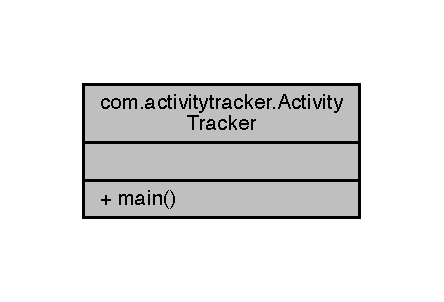
\includegraphics[width=216pt]{classcom_1_1activitytracker_1_1_activity_tracker__coll__graph}
\end{center}
\end{figure}
\subsection*{Static Public Member Functions}
\begin{DoxyCompactItemize}
\item 
static void \hyperlink{classcom_1_1activitytracker_1_1_activity_tracker_a29cfd2975a07afe34e2a3112cbf32dc8}{main} (final String\mbox{[}$\,$\mbox{]} args)
\end{DoxyCompactItemize}


\subsection{Detailed Description}
The main program class. 

Definition at line 28 of file Activity\+Tracker.\+java.



\subsection{Member Function Documentation}
\index{com\+::activitytracker\+::\+Activity\+Tracker@{com\+::activitytracker\+::\+Activity\+Tracker}!main@{main}}
\index{main@{main}!com\+::activitytracker\+::\+Activity\+Tracker@{com\+::activitytracker\+::\+Activity\+Tracker}}
\subsubsection[{\texorpdfstring{main(final String[] args)}{main(final String[] args)}}]{\setlength{\rightskip}{0pt plus 5cm}static void com.\+activitytracker.\+Activity\+Tracker.\+main (
\begin{DoxyParamCaption}
\item[{final String\mbox{[}$\,$\mbox{]}}]{args}
\end{DoxyParamCaption}
)\hspace{0.3cm}{\ttfamily [static]}}\hypertarget{classcom_1_1activitytracker_1_1_activity_tracker_a29cfd2975a07afe34e2a3112cbf32dc8}{}\label{classcom_1_1activitytracker_1_1_activity_tracker_a29cfd2975a07afe34e2a3112cbf32dc8}
The main program entry point. 

Definition at line 33 of file Activity\+Tracker.\+java.


\begin{DoxyCode}
33                                                  \{
34 
35         \textcolor{comment}{// Create singleton instance of DBManager}
36         DBManager dbManager = \textcolor{keyword}{new} DBManager();
37         \textcolor{keywordflow}{if} (!dbManager.init(\textcolor{stringliteral}{"data.db"})) \{
38             System.err.println(\textcolor{stringliteral}{"Failed to initialize DBManager"});
39             System.exit(1);
40         \}
41 
42         \textcolor{comment}{// Set Look and Feel}
43         \textcolor{keywordflow}{try} \{
44             UIManager.setLookAndFeel(\textcolor{keyword}{new} MaterialLookAndFeel());
45         \}
46         \textcolor{keywordflow}{catch} (\textcolor{keyword}{final} UnsupportedLookAndFeelException e) \{
47             e.printStackTrace();
48         \}
49         \textcolor{comment}{// Get desktop resolution of default monitor (in case of multi-monitor setups)}
50         \textcolor{keyword}{final} GraphicsDevice gd = GraphicsEnvironment.getLocalGraphicsEnvironment().getDefaultScreenDevice(
      );
51 
52         \textcolor{keyword}{final} JFrame frame = \textcolor{keyword}{new} JFrame(\textcolor{stringliteral}{"Activity Logger"});
53 
54         \textcolor{keyword}{final} String logoPath = \textcolor{stringliteral}{"./assets/logo.png"};
55         ImageIcon imgIcon = \textcolor{keyword}{new} ImageIcon(ActivityTracker.class.getResource(logoPath));
56         frame.setIconImage(imgIcon.getImage());
57         frame.setContentPane(\textcolor{keyword}{new} LoginWindow((Void) -> \{
58             frame.setContentPane(\textcolor{keyword}{new} MainWindow().rootPanel());
59             frame.validate();
60             frame.repaint();
61         \}).rootPanel());
62         frame.setDefaultCloseOperation(JFrame.EXIT\_ON\_CLOSE);
63         frame.pack();
64 
65         \textcolor{comment}{// Set window size to be 1/2 of screen dimensions}
66         frame.setSize(gd.getDisplayMode().getWidth() / 2, gd.getDisplayMode().getHeight() / 2);
67         frame.setLocationRelativeTo(null); \textcolor{comment}{// Center window}
68         frame.setVisible(\textcolor{keyword}{true});
69     \}
\end{DoxyCode}


The documentation for this class was generated from the following file\+:\begin{DoxyCompactItemize}
\item 
app/src/com/activitytracker/\hyperlink{_activity_tracker_8java}{Activity\+Tracker.\+java}\end{DoxyCompactItemize}

\hypertarget{classcom_1_1activitytracker_1_1_create_user_window}{}\section{com.\+activitytracker.\+Create\+User\+Window Class Reference}
\label{classcom_1_1activitytracker_1_1_create_user_window}\index{com.\+activitytracker.\+Create\+User\+Window@{com.\+activitytracker.\+Create\+User\+Window}}


Inheritance diagram for com.\+activitytracker.\+Create\+User\+Window\+:
\nopagebreak
\begin{figure}[H]
\begin{center}
\leavevmode
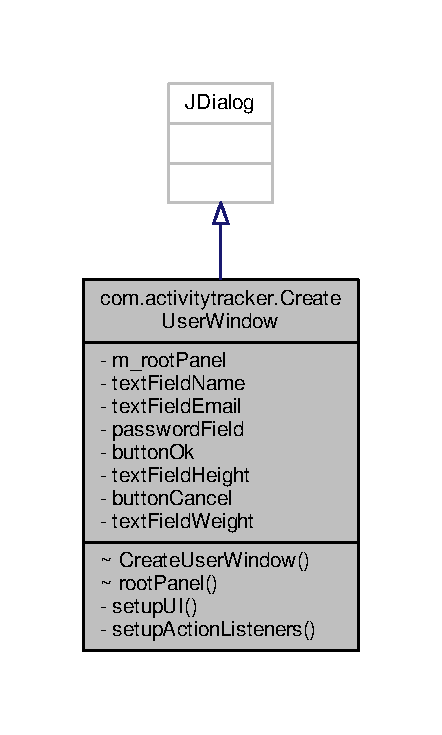
\includegraphics[width=211pt]{classcom_1_1activitytracker_1_1_create_user_window__inherit__graph}
\end{center}
\end{figure}


Collaboration diagram for com.\+activitytracker.\+Create\+User\+Window\+:
\nopagebreak
\begin{figure}[H]
\begin{center}
\leavevmode
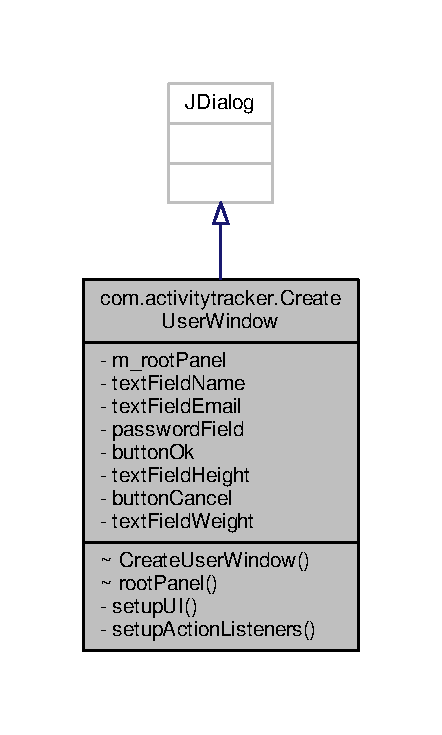
\includegraphics[width=211pt]{classcom_1_1activitytracker_1_1_create_user_window__coll__graph}
\end{center}
\end{figure}
\subsection*{Package Functions}
\begin{DoxyCompactItemize}
\item 
\mbox{\hyperlink{classcom_1_1activitytracker_1_1_create_user_window_a46b8b719c490fe8f658fa7a1f27d0be7}{Create\+User\+Window}} ()
\item 
J\+Panel \mbox{\hyperlink{classcom_1_1activitytracker_1_1_create_user_window_a862f018ae96eb5df7529ff1beb312ff1}{root\+Panel}} ()
\end{DoxyCompactItemize}
\subsection*{Private Member Functions}
\begin{DoxyCompactItemize}
\item 
void \mbox{\hyperlink{classcom_1_1activitytracker_1_1_create_user_window_a41715d85194c6bb84cf6969f771940dc}{setup\+UI}} ()
\item 
void \mbox{\hyperlink{classcom_1_1activitytracker_1_1_create_user_window_a174a05a389ca6f3b7979ac9c5028a3ae}{setup\+Action\+Listeners}} ()
\end{DoxyCompactItemize}
\subsection*{Private Attributes}
\begin{DoxyCompactItemize}
\item 
J\+Panel \mbox{\hyperlink{classcom_1_1activitytracker_1_1_create_user_window_a5a678326afe519b6a2c9e7a2d9eff87c}{m\+\_\+root\+Panel}}
\item 
J\+Text\+Field \mbox{\hyperlink{classcom_1_1activitytracker_1_1_create_user_window_aa2b8cf1781a8a1534dbf5c5b98332c05}{text\+Field\+Name}}
\item 
J\+Text\+Field \mbox{\hyperlink{classcom_1_1activitytracker_1_1_create_user_window_a4f6010631cb7be5a2ae3691bdca31483}{text\+Field\+Email}}
\item 
J\+Password\+Field \mbox{\hyperlink{classcom_1_1activitytracker_1_1_create_user_window_a29be9c267c003ae90731199d8257dc0a}{password\+Field}}
\item 
J\+Button \mbox{\hyperlink{classcom_1_1activitytracker_1_1_create_user_window_aa22864c8baa65b46fe9a7621748d7841}{button\+Ok}}
\item 
J\+Text\+Field \mbox{\hyperlink{classcom_1_1activitytracker_1_1_create_user_window_ac5ce2bc2efbc06d578d93fb3f26aad1c}{text\+Field\+Height}}
\item 
J\+Button \mbox{\hyperlink{classcom_1_1activitytracker_1_1_create_user_window_a975a5cc35d145a3efa4d9e340776ca63}{button\+Cancel}}
\item 
J\+Text\+Field \mbox{\hyperlink{classcom_1_1activitytracker_1_1_create_user_window_ae84b4d977150419bfabc11fbd009392c}{text\+Field\+Weight}}
\end{DoxyCompactItemize}


\subsection{Detailed Description}


Definition at line 11 of file Create\+User\+Window.\+java.



\subsection{Constructor \& Destructor Documentation}
\mbox{\Hypertarget{classcom_1_1activitytracker_1_1_create_user_window_a46b8b719c490fe8f658fa7a1f27d0be7}\label{classcom_1_1activitytracker_1_1_create_user_window_a46b8b719c490fe8f658fa7a1f27d0be7}} 
\index{com\+::activitytracker\+::\+Create\+User\+Window@{com\+::activitytracker\+::\+Create\+User\+Window}!Create\+User\+Window@{Create\+User\+Window}}
\index{Create\+User\+Window@{Create\+User\+Window}!com\+::activitytracker\+::\+Create\+User\+Window@{com\+::activitytracker\+::\+Create\+User\+Window}}
\subsubsection{\texorpdfstring{Create\+User\+Window()}{CreateUserWindow()}}
{\footnotesize\ttfamily com.\+activitytracker.\+Create\+User\+Window.\+Create\+User\+Window (\begin{DoxyParamCaption}{ }\end{DoxyParamCaption})\hspace{0.3cm}{\ttfamily [package]}}



Definition at line 21 of file Create\+User\+Window.\+java.



\subsection{Member Function Documentation}
\mbox{\Hypertarget{classcom_1_1activitytracker_1_1_create_user_window_a862f018ae96eb5df7529ff1beb312ff1}\label{classcom_1_1activitytracker_1_1_create_user_window_a862f018ae96eb5df7529ff1beb312ff1}} 
\index{com\+::activitytracker\+::\+Create\+User\+Window@{com\+::activitytracker\+::\+Create\+User\+Window}!root\+Panel@{root\+Panel}}
\index{root\+Panel@{root\+Panel}!com\+::activitytracker\+::\+Create\+User\+Window@{com\+::activitytracker\+::\+Create\+User\+Window}}
\subsubsection{\texorpdfstring{root\+Panel()}{rootPanel()}}
{\footnotesize\ttfamily J\+Panel com.\+activitytracker.\+Create\+User\+Window.\+root\+Panel (\begin{DoxyParamCaption}{ }\end{DoxyParamCaption})\hspace{0.3cm}{\ttfamily [package]}}



Definition at line 48 of file Create\+User\+Window.\+java.

\mbox{\Hypertarget{classcom_1_1activitytracker_1_1_create_user_window_a174a05a389ca6f3b7979ac9c5028a3ae}\label{classcom_1_1activitytracker_1_1_create_user_window_a174a05a389ca6f3b7979ac9c5028a3ae}} 
\index{com\+::activitytracker\+::\+Create\+User\+Window@{com\+::activitytracker\+::\+Create\+User\+Window}!setup\+Action\+Listeners@{setup\+Action\+Listeners}}
\index{setup\+Action\+Listeners@{setup\+Action\+Listeners}!com\+::activitytracker\+::\+Create\+User\+Window@{com\+::activitytracker\+::\+Create\+User\+Window}}
\subsubsection{\texorpdfstring{setup\+Action\+Listeners()}{setupActionListeners()}}
{\footnotesize\ttfamily void com.\+activitytracker.\+Create\+User\+Window.\+setup\+Action\+Listeners (\begin{DoxyParamCaption}{ }\end{DoxyParamCaption})\hspace{0.3cm}{\ttfamily [private]}}



Definition at line 32 of file Create\+User\+Window.\+java.

\mbox{\Hypertarget{classcom_1_1activitytracker_1_1_create_user_window_a41715d85194c6bb84cf6969f771940dc}\label{classcom_1_1activitytracker_1_1_create_user_window_a41715d85194c6bb84cf6969f771940dc}} 
\index{com\+::activitytracker\+::\+Create\+User\+Window@{com\+::activitytracker\+::\+Create\+User\+Window}!setup\+UI@{setup\+UI}}
\index{setup\+UI@{setup\+UI}!com\+::activitytracker\+::\+Create\+User\+Window@{com\+::activitytracker\+::\+Create\+User\+Window}}
\subsubsection{\texorpdfstring{setup\+U\+I()}{setupUI()}}
{\footnotesize\ttfamily void com.\+activitytracker.\+Create\+User\+Window.\+setup\+UI (\begin{DoxyParamCaption}{ }\end{DoxyParamCaption})\hspace{0.3cm}{\ttfamily [private]}}



Definition at line 27 of file Create\+User\+Window.\+java.



\subsection{Member Data Documentation}
\mbox{\Hypertarget{classcom_1_1activitytracker_1_1_create_user_window_a975a5cc35d145a3efa4d9e340776ca63}\label{classcom_1_1activitytracker_1_1_create_user_window_a975a5cc35d145a3efa4d9e340776ca63}} 
\index{com\+::activitytracker\+::\+Create\+User\+Window@{com\+::activitytracker\+::\+Create\+User\+Window}!button\+Cancel@{button\+Cancel}}
\index{button\+Cancel@{button\+Cancel}!com\+::activitytracker\+::\+Create\+User\+Window@{com\+::activitytracker\+::\+Create\+User\+Window}}
\subsubsection{\texorpdfstring{button\+Cancel}{buttonCancel}}
{\footnotesize\ttfamily J\+Button com.\+activitytracker.\+Create\+User\+Window.\+button\+Cancel\hspace{0.3cm}{\ttfamily [private]}}



Definition at line 18 of file Create\+User\+Window.\+java.

\mbox{\Hypertarget{classcom_1_1activitytracker_1_1_create_user_window_aa22864c8baa65b46fe9a7621748d7841}\label{classcom_1_1activitytracker_1_1_create_user_window_aa22864c8baa65b46fe9a7621748d7841}} 
\index{com\+::activitytracker\+::\+Create\+User\+Window@{com\+::activitytracker\+::\+Create\+User\+Window}!button\+Ok@{button\+Ok}}
\index{button\+Ok@{button\+Ok}!com\+::activitytracker\+::\+Create\+User\+Window@{com\+::activitytracker\+::\+Create\+User\+Window}}
\subsubsection{\texorpdfstring{button\+Ok}{buttonOk}}
{\footnotesize\ttfamily J\+Button com.\+activitytracker.\+Create\+User\+Window.\+button\+Ok\hspace{0.3cm}{\ttfamily [private]}}



Definition at line 16 of file Create\+User\+Window.\+java.

\mbox{\Hypertarget{classcom_1_1activitytracker_1_1_create_user_window_a5a678326afe519b6a2c9e7a2d9eff87c}\label{classcom_1_1activitytracker_1_1_create_user_window_a5a678326afe519b6a2c9e7a2d9eff87c}} 
\index{com\+::activitytracker\+::\+Create\+User\+Window@{com\+::activitytracker\+::\+Create\+User\+Window}!m\+\_\+root\+Panel@{m\+\_\+root\+Panel}}
\index{m\+\_\+root\+Panel@{m\+\_\+root\+Panel}!com\+::activitytracker\+::\+Create\+User\+Window@{com\+::activitytracker\+::\+Create\+User\+Window}}
\subsubsection{\texorpdfstring{m\+\_\+root\+Panel}{m\_rootPanel}}
{\footnotesize\ttfamily J\+Panel com.\+activitytracker.\+Create\+User\+Window.\+m\+\_\+root\+Panel\hspace{0.3cm}{\ttfamily [private]}}



Definition at line 12 of file Create\+User\+Window.\+java.

\mbox{\Hypertarget{classcom_1_1activitytracker_1_1_create_user_window_a29be9c267c003ae90731199d8257dc0a}\label{classcom_1_1activitytracker_1_1_create_user_window_a29be9c267c003ae90731199d8257dc0a}} 
\index{com\+::activitytracker\+::\+Create\+User\+Window@{com\+::activitytracker\+::\+Create\+User\+Window}!password\+Field@{password\+Field}}
\index{password\+Field@{password\+Field}!com\+::activitytracker\+::\+Create\+User\+Window@{com\+::activitytracker\+::\+Create\+User\+Window}}
\subsubsection{\texorpdfstring{password\+Field}{passwordField}}
{\footnotesize\ttfamily J\+Password\+Field com.\+activitytracker.\+Create\+User\+Window.\+password\+Field\hspace{0.3cm}{\ttfamily [private]}}



Definition at line 15 of file Create\+User\+Window.\+java.

\mbox{\Hypertarget{classcom_1_1activitytracker_1_1_create_user_window_a4f6010631cb7be5a2ae3691bdca31483}\label{classcom_1_1activitytracker_1_1_create_user_window_a4f6010631cb7be5a2ae3691bdca31483}} 
\index{com\+::activitytracker\+::\+Create\+User\+Window@{com\+::activitytracker\+::\+Create\+User\+Window}!text\+Field\+Email@{text\+Field\+Email}}
\index{text\+Field\+Email@{text\+Field\+Email}!com\+::activitytracker\+::\+Create\+User\+Window@{com\+::activitytracker\+::\+Create\+User\+Window}}
\subsubsection{\texorpdfstring{text\+Field\+Email}{textFieldEmail}}
{\footnotesize\ttfamily J\+Text\+Field com.\+activitytracker.\+Create\+User\+Window.\+text\+Field\+Email\hspace{0.3cm}{\ttfamily [private]}}



Definition at line 14 of file Create\+User\+Window.\+java.

\mbox{\Hypertarget{classcom_1_1activitytracker_1_1_create_user_window_ac5ce2bc2efbc06d578d93fb3f26aad1c}\label{classcom_1_1activitytracker_1_1_create_user_window_ac5ce2bc2efbc06d578d93fb3f26aad1c}} 
\index{com\+::activitytracker\+::\+Create\+User\+Window@{com\+::activitytracker\+::\+Create\+User\+Window}!text\+Field\+Height@{text\+Field\+Height}}
\index{text\+Field\+Height@{text\+Field\+Height}!com\+::activitytracker\+::\+Create\+User\+Window@{com\+::activitytracker\+::\+Create\+User\+Window}}
\subsubsection{\texorpdfstring{text\+Field\+Height}{textFieldHeight}}
{\footnotesize\ttfamily J\+Text\+Field com.\+activitytracker.\+Create\+User\+Window.\+text\+Field\+Height\hspace{0.3cm}{\ttfamily [private]}}



Definition at line 17 of file Create\+User\+Window.\+java.

\mbox{\Hypertarget{classcom_1_1activitytracker_1_1_create_user_window_aa2b8cf1781a8a1534dbf5c5b98332c05}\label{classcom_1_1activitytracker_1_1_create_user_window_aa2b8cf1781a8a1534dbf5c5b98332c05}} 
\index{com\+::activitytracker\+::\+Create\+User\+Window@{com\+::activitytracker\+::\+Create\+User\+Window}!text\+Field\+Name@{text\+Field\+Name}}
\index{text\+Field\+Name@{text\+Field\+Name}!com\+::activitytracker\+::\+Create\+User\+Window@{com\+::activitytracker\+::\+Create\+User\+Window}}
\subsubsection{\texorpdfstring{text\+Field\+Name}{textFieldName}}
{\footnotesize\ttfamily J\+Text\+Field com.\+activitytracker.\+Create\+User\+Window.\+text\+Field\+Name\hspace{0.3cm}{\ttfamily [private]}}



Definition at line 13 of file Create\+User\+Window.\+java.

\mbox{\Hypertarget{classcom_1_1activitytracker_1_1_create_user_window_ae84b4d977150419bfabc11fbd009392c}\label{classcom_1_1activitytracker_1_1_create_user_window_ae84b4d977150419bfabc11fbd009392c}} 
\index{com\+::activitytracker\+::\+Create\+User\+Window@{com\+::activitytracker\+::\+Create\+User\+Window}!text\+Field\+Weight@{text\+Field\+Weight}}
\index{text\+Field\+Weight@{text\+Field\+Weight}!com\+::activitytracker\+::\+Create\+User\+Window@{com\+::activitytracker\+::\+Create\+User\+Window}}
\subsubsection{\texorpdfstring{text\+Field\+Weight}{textFieldWeight}}
{\footnotesize\ttfamily J\+Text\+Field com.\+activitytracker.\+Create\+User\+Window.\+text\+Field\+Weight\hspace{0.3cm}{\ttfamily [private]}}



Definition at line 19 of file Create\+User\+Window.\+java.



The documentation for this class was generated from the following file\+:\begin{DoxyCompactItemize}
\item 
app/src/com/activitytracker/\mbox{\hyperlink{_create_user_window_8java}{Create\+User\+Window.\+java}}\end{DoxyCompactItemize}

\hypertarget{classcom_1_1activitytracker_1_1_d_b_manager}{}\section{com.\+activitytracker.\+D\+B\+Manager Class Reference}
\label{classcom_1_1activitytracker_1_1_d_b_manager}\index{com.\+activitytracker.\+D\+B\+Manager@{com.\+activitytracker.\+D\+B\+Manager}}


Collaboration diagram for com.\+activitytracker.\+D\+B\+Manager\+:
\nopagebreak
\begin{figure}[H]
\begin{center}
\leavevmode
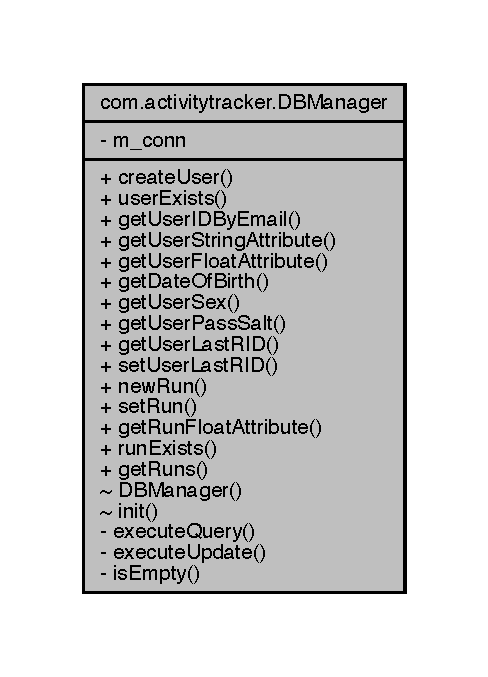
\includegraphics[width=234pt]{classcom_1_1activitytracker_1_1_d_b_manager__coll__graph}
\end{center}
\end{figure}
\subsection*{Public Member Functions}
\begin{DoxyCompactItemize}
\item 
void \mbox{\hyperlink{classcom_1_1activitytracker_1_1_d_b_manager_a39ef296348c7bfacf965b3417655f4e5}{create\+User}} (final String name, final String email\+Address, final int D\+O\+B\+Year, final int D\+O\+B\+Month, final int D\+O\+B\+Day, final User.\+Sex sex, final float height, final float weight, final \mbox{\hyperlink{classcom_1_1activitytracker_1_1_secure_string}{Secure\+String}} secure\+Password)  throws Assertion\+Error 
\item 
boolean \mbox{\hyperlink{classcom_1_1activitytracker_1_1_d_b_manager_af05d79f33ecf2920a67d1b9cf82c079f}{user\+Exists}} (final String email\+Address)
\item 
int \mbox{\hyperlink{classcom_1_1activitytracker_1_1_d_b_manager_a195dcdeabdd00facb19d720976dd3f53}{get\+User\+I\+D\+By\+Email}} (final String email\+Address)
\item 
String \mbox{\hyperlink{classcom_1_1activitytracker_1_1_d_b_manager_a20f726c054d6c8a6fc3ce629d87f1114}{get\+User\+String\+Attribute}} (final \mbox{\hyperlink{enumcom_1_1activitytracker_1_1_user_attribute}{User\+Attribute}} attribute, final int id)
\item 
float \mbox{\hyperlink{classcom_1_1activitytracker_1_1_d_b_manager_a98df66254bec4d74b29cfe468a9fc794}{get\+User\+Float\+Attribute}} (final \mbox{\hyperlink{enumcom_1_1activitytracker_1_1_user_attribute}{User\+Attribute}} attribute, final int id)
\item 
Date \mbox{\hyperlink{classcom_1_1activitytracker_1_1_d_b_manager_a0576baf67b45c7d2d0ba369052e4404e}{get\+Date\+Of\+Birth}} (final int id)
\item 
User.\+Sex \mbox{\hyperlink{classcom_1_1activitytracker_1_1_d_b_manager_a4e695c111b877cfd1d918602551f65a1}{get\+User\+Sex}} (final int id)
\item 
byte \mbox{[}$\,$\mbox{]} \mbox{\hyperlink{classcom_1_1activitytracker_1_1_d_b_manager_aeab864b072cc08c0521e80ae1f459ca7}{get\+User\+Pass\+Salt}} (final int id)
\item 
int \mbox{\hyperlink{classcom_1_1activitytracker_1_1_d_b_manager_aab14c61b3f3a17bdea10cab1b5fd9337}{get\+User\+Last\+R\+ID}} (final int id)
\item 
void \mbox{\hyperlink{classcom_1_1activitytracker_1_1_d_b_manager_a93b7fc4c2d0083e125852d84f087a8d3}{set\+User\+Last\+R\+ID}} (final int id, final int last\+R\+ID)
\item 
int \mbox{\hyperlink{classcom_1_1activitytracker_1_1_d_b_manager_a05b742f583167f6ce00eb8415c43fc1c}{new\+Run}} (final int user\+ID, final int year, final int month, final int day, final float duration, final float distance, final float altitude\+\_\+ascended, final float altitude\+\_\+descended)
\item 
void \mbox{\hyperlink{classcom_1_1activitytracker_1_1_d_b_manager_a72282377a552ce4ce371abff02e312f2}{set\+Run}} (final int r\+ID, final float duration, final float distance, final float altitude\+\_\+ascended, final float altitude\+\_\+descended)
\item 
float \mbox{\hyperlink{classcom_1_1activitytracker_1_1_d_b_manager_a666452f1e5862f90c06b0beb9a9fcfdd}{get\+Run\+Float\+Attribute}} (final \mbox{\hyperlink{enumcom_1_1activitytracker_1_1_run_attribute}{Run\+Attribute}} attribute, final int r\+ID)
\item 
boolean \mbox{\hyperlink{classcom_1_1activitytracker_1_1_d_b_manager_a723ac1c573bacdd0b62894357bd65a9b}{run\+Exists}} (final int r\+ID)
\end{DoxyCompactItemize}
\subsection*{Package Functions}
\begin{DoxyCompactItemize}
\item 
\mbox{\hyperlink{classcom_1_1activitytracker_1_1_d_b_manager_ac1f558ef56fe02d74fe103a473a15bb5}{D\+B\+Manager}} ()
\item 
boolean \mbox{\hyperlink{classcom_1_1activitytracker_1_1_d_b_manager_a41df4600bb5901a26a4ea6a7108a70b9}{init}} (final String db\+U\+RL)
\end{DoxyCompactItemize}
\subsection*{Private Member Functions}
\begin{DoxyCompactItemize}
\item 
Result\+Set \mbox{\hyperlink{classcom_1_1activitytracker_1_1_d_b_manager_adef71a18dc05536d80e83311841e1953}{execute\+Query}} (final String sql\+Query)
\item 
boolean \mbox{\hyperlink{classcom_1_1activitytracker_1_1_d_b_manager_a382397e2bdf309901d1c80ff66be69b7}{execute\+Update}} (final String sql\+Query)
\item 
boolean \mbox{\hyperlink{classcom_1_1activitytracker_1_1_d_b_manager_af9ab112f840e3c803b6b28a2f1a15215}{is\+Empty}} ()
\end{DoxyCompactItemize}
\subsection*{Private Attributes}
\begin{DoxyCompactItemize}
\item 
Connection \mbox{\hyperlink{classcom_1_1activitytracker_1_1_d_b_manager_a064088d13ac09eb147fdc19268771521}{m\+\_\+conn}} = null
\end{DoxyCompactItemize}


\subsection{Detailed Description}
Singleton class for the database. All classes and methods that interact with the database will use a method in this class.

Many times we are faced with the \char`\"{}chicken and egg\char`\"{} problem where we wish to create an object that is populated with information from the database. So the question one faces is, "does the object\textquotesingle{}s constructor query the database (through the \mbox{\hyperlink{classcom_1_1activitytracker_1_1_d_b_manager}{D\+B\+Manager}} class, of course) for each attribute of the object that it wishes to retrieve, or do we directly interact with a \mbox{\hyperlink{classcom_1_1activitytracker_1_1_d_b_manager}{D\+B\+Manager}} method which will then return a \mbox{\hyperlink{classcom_1_1activitytracker_1_1_user}{User}} or \mbox{\hyperlink{classcom_1_1activitytracker_1_1_run}{Run}} object, for example?" We have decided to use the former methodology, with \mbox{\hyperlink{classcom_1_1activitytracker_1_1_d_b_manager}{D\+B\+Manager}} methods being as general as possible, and often accepting enum types which then are put into a switch to create the specific S\+QL query we wish to execute. This works best when all data returned is of the same data type (for example, the Workout class will have three float attributes at the time of writing so we use one method with return type of float for returning Workout attributes). This does not work as well when the object requires data of multiple types --- for example, the \mbox{\hyperlink{classcom_1_1activitytracker_1_1_user}{User}} class. In this case, we have split the \mbox{\hyperlink{classcom_1_1activitytracker_1_1_d_b_manager}{D\+B\+Manager}} methods into a single method for each attribute being returned.

Polymorphism could theoretically be used here to simply have a return type of Object, however this is not flexible and requires casting {\itshape all} returned data to the correct type in the invoking method. 

Definition at line 25 of file D\+B\+Manager.\+java.



\subsection{Constructor \& Destructor Documentation}
\mbox{\Hypertarget{classcom_1_1activitytracker_1_1_d_b_manager_ac1f558ef56fe02d74fe103a473a15bb5}\label{classcom_1_1activitytracker_1_1_d_b_manager_ac1f558ef56fe02d74fe103a473a15bb5}} 
\index{com\+::activitytracker\+::\+D\+B\+Manager@{com\+::activitytracker\+::\+D\+B\+Manager}!D\+B\+Manager@{D\+B\+Manager}}
\index{D\+B\+Manager@{D\+B\+Manager}!com\+::activitytracker\+::\+D\+B\+Manager@{com\+::activitytracker\+::\+D\+B\+Manager}}
\subsubsection{\texorpdfstring{D\+B\+Manager()}{DBManager()}}
{\footnotesize\ttfamily com.\+activitytracker.\+D\+B\+Manager.\+D\+B\+Manager (\begin{DoxyParamCaption}{ }\end{DoxyParamCaption})\hspace{0.3cm}{\ttfamily [package]}}

Creates a new \mbox{\hyperlink{classcom_1_1activitytracker_1_1_d_b_manager}{D\+B\+Manager}} object.

This should only be called once, from the main program, as \mbox{\hyperlink{classcom_1_1activitytracker_1_1_d_b_manager}{D\+B\+Manager}} is meant to be a {\itshape singleton} class.

This constructor takes no parameters as verification of the S\+Q\+Lite database is done in the \mbox{\hyperlink{classcom_1_1activitytracker_1_1_d_b_manager_a41df4600bb5901a26a4ea6a7108a70b9}{init()}} method of this class, which returns information about whether the initialization was successful or not. 

Definition at line 42 of file D\+B\+Manager.\+java.


\begin{DoxyCode}
42                 \{
43     \}
\end{DoxyCode}


\subsection{Member Function Documentation}
\mbox{\Hypertarget{classcom_1_1activitytracker_1_1_d_b_manager_a39ef296348c7bfacf965b3417655f4e5}\label{classcom_1_1activitytracker_1_1_d_b_manager_a39ef296348c7bfacf965b3417655f4e5}} 
\index{com\+::activitytracker\+::\+D\+B\+Manager@{com\+::activitytracker\+::\+D\+B\+Manager}!create\+User@{create\+User}}
\index{create\+User@{create\+User}!com\+::activitytracker\+::\+D\+B\+Manager@{com\+::activitytracker\+::\+D\+B\+Manager}}
\subsubsection{\texorpdfstring{create\+User()}{createUser()}}
{\footnotesize\ttfamily void com.\+activitytracker.\+D\+B\+Manager.\+create\+User (\begin{DoxyParamCaption}\item[{final String}]{name,  }\item[{final String}]{email\+Address,  }\item[{final int}]{D\+O\+B\+Year,  }\item[{final int}]{D\+O\+B\+Month,  }\item[{final int}]{D\+O\+B\+Day,  }\item[{final User.\+Sex}]{sex,  }\item[{final float}]{height,  }\item[{final float}]{weight,  }\item[{final \mbox{\hyperlink{classcom_1_1activitytracker_1_1_secure_string}{Secure\+String}}}]{secure\+Password }\end{DoxyParamCaption}) throws Assertion\+Error}

Adds a row for a user to the Users table in the S\+Q\+Lite database for the app.

Requires that the database tables exist and are in the correct format. If the user exists in the database this method raises an Assertion\+Error exception.


\begin{DoxyParams}{Parameters}
{\em name} & User\textquotesingle{}s name \\
\hline
{\em email\+Address} & User\textquotesingle{}s email address; used to authenticate \\
\hline
{\em D\+O\+B\+Year} & The year the user was born \\
\hline
{\em D\+O\+B\+Month} & The month the user was born \\
\hline
{\em D\+O\+B\+Day} & The day of month the user was born \\
\hline
{\em sex} & The user\textquotesingle{}s sex; is either \mbox{\hyperlink{enumcom_1_1activitytracker_1_1_user_1_1_sex_ad3b626a38bd4615eb621d75b939f412d}{User.\+Sex.\+M\+A\+LE}} or \mbox{\hyperlink{enumcom_1_1activitytracker_1_1_user_1_1_sex_a5c22ece8a4df71ed5202cd492990a752}{User.\+Sex.\+F\+E\+M\+A\+LE}} \\
\hline
{\em height} & Floating point number of the user\textquotesingle{}s height in metres \\
\hline
{\em weight} & Floating point number of the user\textquotesingle{}s weight in kilograms \\
\hline
{\em secure\+Password} & A \mbox{\hyperlink{classcom_1_1activitytracker_1_1_secure_string}{Secure\+String}} object containing the user\textquotesingle{}s password, encrypted \\
\hline
\end{DoxyParams}


Definition at line 61 of file D\+B\+Manager.\+java.


\begin{DoxyCode}
63                                                                                                         \{
64 
65         \textcolor{keywordflow}{if} (!\mbox{\hyperlink{classcom_1_1activitytracker_1_1_d_b_manager_af05d79f33ecf2920a67d1b9cf82c079f}{userExists}}(emailAddress)) \{
66             String sqlQuery = \textcolor{stringliteral}{"INSERT INTO Users ("} +
67                     \textcolor{stringliteral}{"email\_address, "} +
68                     \textcolor{stringliteral}{"name, "} +
69                     \textcolor{stringliteral}{"date\_of\_birth, "} +
70                     \textcolor{stringliteral}{"sex, "} +
71                     \textcolor{stringliteral}{"height, "} +
72                     \textcolor{stringliteral}{"weight,"} +
73                     \textcolor{stringliteral}{"password\_hash,"} +
74                     \textcolor{stringliteral}{"password\_salt,"} +
75                     \textcolor{stringliteral}{"created\_at"} +
76                     \textcolor{stringliteral}{") VALUES (?, ?, ?, ?, ?, ?, ?, ?, ?)"};
77             byte sexByte = sex.equals(User.Sex.MALE) ? (byte) 1 : (byte) 0;
78             java.sql.Date currentTime = \textcolor{keyword}{new} java.sql.Date(System.currentTimeMillis());
79             Calendar c = Calendar.getInstance();
80             c.set(DOBYear, DOBMonth, DOBDay);
81             java.sql.Date dateOfBirth = \textcolor{keyword}{new} java.sql.Date(
82                     c.get(Calendar.YEAR),
83                     c.get(Calendar.MONTH),
84                     c.get(Calendar.DAY\_OF\_MONTH)
85             );
86 
87             \textcolor{keywordflow}{try} \{
88                 PreparedStatement stmt = \mbox{\hyperlink{classcom_1_1activitytracker_1_1_d_b_manager_a064088d13ac09eb147fdc19268771521}{m\_conn}}.prepareStatement(sqlQuery);
89                 stmt.setString(1, emailAddress);
90                 stmt.setString(2, name);
91                 stmt.setDate(3, dateOfBirth);
92                 stmt.setByte(4, sexByte);
93                 stmt.setFloat(5, height);
94                 stmt.setFloat(6, weight);
95                 stmt.setString(7, securePassword.toString());
96                 stmt.setBytes(8, securePassword.getSalt());
97                 stmt.setDate(9, currentTime);
98 
99                 \textcolor{keywordflow}{if} (stmt.executeUpdate() != 1) \{
100                     System.err.println(\textcolor{stringliteral}{"User not added to database."});
101                 \}
102 
103                 stmt.close();
104             \}
105             \textcolor{keywordflow}{catch} (\textcolor{keyword}{final} SQLException e) \{
106                 System.err.println(e.getMessage());
107             \}
108         \}
109         \textcolor{keywordflow}{else} \{
110             \textcolor{keywordflow}{throw} \textcolor{keyword}{new} AssertionError(\textcolor{stringliteral}{"User with email address '"} + emailAddress + \textcolor{stringliteral}{"' already exists."});
111         \}
112     \}
\end{DoxyCode}
\mbox{\Hypertarget{classcom_1_1activitytracker_1_1_d_b_manager_adef71a18dc05536d80e83311841e1953}\label{classcom_1_1activitytracker_1_1_d_b_manager_adef71a18dc05536d80e83311841e1953}} 
\index{com\+::activitytracker\+::\+D\+B\+Manager@{com\+::activitytracker\+::\+D\+B\+Manager}!execute\+Query@{execute\+Query}}
\index{execute\+Query@{execute\+Query}!com\+::activitytracker\+::\+D\+B\+Manager@{com\+::activitytracker\+::\+D\+B\+Manager}}
\subsubsection{\texorpdfstring{execute\+Query()}{executeQuery()}}
{\footnotesize\ttfamily Result\+Set com.\+activitytracker.\+D\+B\+Manager.\+execute\+Query (\begin{DoxyParamCaption}\item[{final String}]{sql\+Query }\end{DoxyParamCaption})\hspace{0.3cm}{\ttfamily [private]}}

A wrapper method for processing {\itshape safe} S\+QL queries.

By safe we mean that the S\+QL query string is entirely hard-\/coded in the program source code. In other words, no user input is added. This is an important distinction as the former may leave the application vulnerable to S\+QL injection.

In such cases, a S\+QL Prepared\+Statement should be used.


\begin{DoxyParams}{Parameters}
{\em sql\+Query} & The S\+QL code to be executed. Must be a {\itshape S\+E\+L\+E\+CT} statement.\\
\hline
\end{DoxyParams}
\begin{DoxyReturn}{Returns}
This method returns a Result\+Set containing the returned row(s) and/or column(s) of the S\+QL query that was executed. 
\end{DoxyReturn}


Definition at line 680 of file D\+B\+Manager.\+java.


\begin{DoxyCode}
680                                                           \{
681         ResultSet res = null;
682 
683         \textcolor{keywordflow}{try} \{
684             Statement stmt = \mbox{\hyperlink{classcom_1_1activitytracker_1_1_d_b_manager_a064088d13ac09eb147fdc19268771521}{m\_conn}}.createStatement();
685             res = stmt.executeQuery(sqlQuery);
686             stmt.close();
687         \}
688         \textcolor{keywordflow}{catch} (\textcolor{keyword}{final} SQLException e) \{
689             System.err.println(e.getMessage());
690         \}
691 
692         \textcolor{keywordflow}{return} res;
693     \}
\end{DoxyCode}
\mbox{\Hypertarget{classcom_1_1activitytracker_1_1_d_b_manager_a382397e2bdf309901d1c80ff66be69b7}\label{classcom_1_1activitytracker_1_1_d_b_manager_a382397e2bdf309901d1c80ff66be69b7}} 
\index{com\+::activitytracker\+::\+D\+B\+Manager@{com\+::activitytracker\+::\+D\+B\+Manager}!execute\+Update@{execute\+Update}}
\index{execute\+Update@{execute\+Update}!com\+::activitytracker\+::\+D\+B\+Manager@{com\+::activitytracker\+::\+D\+B\+Manager}}
\subsubsection{\texorpdfstring{execute\+Update()}{executeUpdate()}}
{\footnotesize\ttfamily boolean com.\+activitytracker.\+D\+B\+Manager.\+execute\+Update (\begin{DoxyParamCaption}\item[{final String}]{sql\+Query }\end{DoxyParamCaption})\hspace{0.3cm}{\ttfamily [private]}}

A wrapper method for processing {\itshape safe} S\+QL queries.

By safe we mean that the S\+QL query string is entirely hard-\/coded in the program source code. In other words, no user input is added. This is an important distinction as the former may leave the application vulnerable to S\+QL injection.

In such cases, a S\+QL Prepared\+Statement should be used.


\begin{DoxyParams}{Parameters}
{\em sql\+Query} & The S\+QL code to be executed. Must be an {\itshape I\+N\+S\+E\+RT} or {\itshape U\+P\+D\+A\+TE} statement.\\
\hline
\end{DoxyParams}
\begin{DoxyReturn}{Returns}
This method returns a boolean indicating if the query was successful. 
\end{DoxyReturn}


Definition at line 708 of file D\+B\+Manager.\+java.


\begin{DoxyCode}
708                                                          \{
709         \textcolor{keywordflow}{try} \{
710             Statement stmt = \mbox{\hyperlink{classcom_1_1activitytracker_1_1_d_b_manager_a064088d13ac09eb147fdc19268771521}{m\_conn}}.createStatement();
711             stmt.executeUpdate(sqlQuery);
712             stmt.close();
713         \}
714         \textcolor{keywordflow}{catch} (\textcolor{keyword}{final} SQLException e) \{
715             System.err.println(e.getMessage());
716             \textcolor{keywordflow}{return} \textcolor{keyword}{false};
717         \}
718 
719         \textcolor{keywordflow}{return} \textcolor{keyword}{true};
720     \}
\end{DoxyCode}
\mbox{\Hypertarget{classcom_1_1activitytracker_1_1_d_b_manager_a0576baf67b45c7d2d0ba369052e4404e}\label{classcom_1_1activitytracker_1_1_d_b_manager_a0576baf67b45c7d2d0ba369052e4404e}} 
\index{com\+::activitytracker\+::\+D\+B\+Manager@{com\+::activitytracker\+::\+D\+B\+Manager}!get\+Date\+Of\+Birth@{get\+Date\+Of\+Birth}}
\index{get\+Date\+Of\+Birth@{get\+Date\+Of\+Birth}!com\+::activitytracker\+::\+D\+B\+Manager@{com\+::activitytracker\+::\+D\+B\+Manager}}
\subsubsection{\texorpdfstring{get\+Date\+Of\+Birth()}{getDateOfBirth()}}
{\footnotesize\ttfamily Date com.\+activitytracker.\+D\+B\+Manager.\+get\+Date\+Of\+Birth (\begin{DoxyParamCaption}\item[{final int}]{id }\end{DoxyParamCaption})}

Retrieves the user\textquotesingle{}s date of birth (D\+OB) from the database.

At the time of writing, this method is only being used in the \mbox{\hyperlink{classcom_1_1activitytracker_1_1_user}{User}} constructor.


\begin{DoxyParams}{Parameters}
{\em id} & Unique ID used to associate information in the database to this user.\\
\hline
\end{DoxyParams}
\begin{DoxyReturn}{Returns}
This method returns a Date object containing the user\textquotesingle{}s D\+OB (i.\+e., year, month, day). 
\end{DoxyReturn}


Definition at line 298 of file D\+B\+Manager.\+java.


\begin{DoxyCode}
298                                              \{
299         Date DOB;
300         java.sql.Date DOBResult;
301         ResultSet res;
302         String sqlQuery = \textcolor{stringliteral}{"SELECT date\_of\_birth FROM Users WHERE id=?"};
303         \textcolor{keywordflow}{try} \{
304             PreparedStatement stmt = \mbox{\hyperlink{classcom_1_1activitytracker_1_1_d_b_manager_a064088d13ac09eb147fdc19268771521}{m\_conn}}.prepareStatement(sqlQuery);
305             stmt.setInt(1, \textcolor{keywordtype}{id});
306             res = stmt.executeQuery();
307             DOBResult = res.getDate(\textcolor{stringliteral}{"date\_of\_birth"});
308 
309             stmt.close();
310         \}
311         \textcolor{keywordflow}{catch} (\textcolor{keyword}{final} SQLException e) \{
312             System.err.println(e.getMessage());
313             \textcolor{keywordflow}{return} null;
314         \}
315         DOB = \textcolor{keyword}{new} Date(DOBResult.getYear(), DOBResult.getMonth(), DOBResult.getDay());
316 
317         \textcolor{keywordflow}{return} DOB;
318     \}
\end{DoxyCode}
\mbox{\Hypertarget{classcom_1_1activitytracker_1_1_d_b_manager_a666452f1e5862f90c06b0beb9a9fcfdd}\label{classcom_1_1activitytracker_1_1_d_b_manager_a666452f1e5862f90c06b0beb9a9fcfdd}} 
\index{com\+::activitytracker\+::\+D\+B\+Manager@{com\+::activitytracker\+::\+D\+B\+Manager}!get\+Run\+Float\+Attribute@{get\+Run\+Float\+Attribute}}
\index{get\+Run\+Float\+Attribute@{get\+Run\+Float\+Attribute}!com\+::activitytracker\+::\+D\+B\+Manager@{com\+::activitytracker\+::\+D\+B\+Manager}}
\subsubsection{\texorpdfstring{get\+Run\+Float\+Attribute()}{getRunFloatAttribute()}}
{\footnotesize\ttfamily float com.\+activitytracker.\+D\+B\+Manager.\+get\+Run\+Float\+Attribute (\begin{DoxyParamCaption}\item[{final \mbox{\hyperlink{enumcom_1_1activitytracker_1_1_run_attribute}{Run\+Attribute}}}]{attribute,  }\item[{final int}]{r\+ID }\end{DoxyParamCaption})}

Retrieves a run\textquotesingle{}s attribute as a floating point number, where applicable, from the database.

This method accepts a \mbox{\hyperlink{enumcom_1_1activitytracker_1_1_run_attribute}{Run\+Attribute}} enumeration type to specify what attribute it is returning from the database. Only certain attributes are accepted by this method, namely those that are stored as real values. Attributes stored as other data types should use the appropriate accessor method.


\begin{DoxyParams}{Parameters}
{\em attribute} & The attribute that the method is supposed to query the DB for and return the value of. Note that only certain \mbox{\hyperlink{enumcom_1_1activitytracker_1_1_run_attribute}{Run\+Attribute}} types are supported in this method.
\begin{DoxyItemize}
\item When {\itshape attribute} is \mbox{\hyperlink{enumcom_1_1activitytracker_1_1_run_attribute_a7adf133b2a62f1f99ffc2adfb7097ec9}{Run\+Attribute.\+D\+U\+R\+A\+T\+I\+ON}}, the run\textquotesingle{}s duration is returned.
\item When {\itshape attribute} is \mbox{\hyperlink{enumcom_1_1activitytracker_1_1_run_attribute_a90ee541e68e458a0bb3f5ea45fd46ec0}{Run\+Attribute.\+D\+I\+S\+T\+A\+N\+CE}}, the run\textquotesingle{}s cumulative distance is returned in metres.
\item When {\itshape attribute} is \mbox{\hyperlink{enumcom_1_1activitytracker_1_1_run_attribute_abcfe85bf48187d67842a0525c1bcc0af}{Run\+Attribute.\+A\+L\+T\+I\+T\+U\+D\+E\+\_\+\+A\+S\+C\+E\+N\+D\+ED}}, the run\textquotesingle{}s cumulative altitude climbed is returned in metres
\item When {\itshape attribute} is \mbox{\hyperlink{enumcom_1_1activitytracker_1_1_run_attribute_a337a68867cfdb8ec7a17c318ad8b216b}{Run\+Attribute.\+A\+L\+T\+I\+T\+U\+D\+E\+\_\+\+D\+E\+S\+C\+E\+N\+D\+ED}}, the run\textquotesingle{}s cumulative altitude descended is returned in metres 
\end{DoxyItemize}\\
\hline
{\em r\+ID} & Unique ID corresponding to the row in the Runs table that we wish to query. If such an ID does not exist, {\itshape 0.\+0f} will be returned.\\
\hline
\end{DoxyParams}
\begin{DoxyReturn}{Returns}
This method returns a float containing run attribute as specified by the {\itshape attribute} parameter. 
\end{DoxyReturn}


Definition at line 585 of file D\+B\+Manager.\+java.


\begin{DoxyCode}
585                                                                                    \{
586         ResultSet res;
587         PreparedStatement stmt;
588         String sqlQuery, columnLabel;
589         \textcolor{keywordtype}{float} attrVal = 0.0f;
590         \textcolor{keywordflow}{switch} (attribute) \{
591             \textcolor{keywordflow}{case} DURATION:
592                 columnLabel = \textcolor{stringliteral}{"duration"};
593                 sqlQuery = \textcolor{stringliteral}{"SELECT "} + columnLabel + \textcolor{stringliteral}{" FROM Runs WHERE id=?"};
594                 \textcolor{keywordflow}{break};
595             \textcolor{keywordflow}{case} DISTANCE:
596                 columnLabel = \textcolor{stringliteral}{"distance"};
597                 sqlQuery = \textcolor{stringliteral}{"SELECT "} + columnLabel + \textcolor{stringliteral}{" FROM Runs WHERE id=?"};
598                 \textcolor{keywordflow}{break};
599             \textcolor{keywordflow}{case} ALTITUDE\_ASCENDED:
600                 columnLabel = \textcolor{stringliteral}{"altitude\_ascended"};
601                 sqlQuery = \textcolor{stringliteral}{"SELECT "} + columnLabel + \textcolor{stringliteral}{" FROM Runs WHERE id=?"};
602                 \textcolor{keywordflow}{break};
603             \textcolor{keywordflow}{case} ALTITUDE\_DESCENDED:
604                 columnLabel = \textcolor{stringliteral}{"altitude\_descended"};
605                 sqlQuery = \textcolor{stringliteral}{"SELECT "} + columnLabel + \textcolor{stringliteral}{" FROM Runs WHERE id=?"};
606                 \textcolor{keywordflow}{break};
607             \textcolor{keywordflow}{default}:
608                 \textcolor{keywordflow}{return} attrVal;
609         \}
610         \textcolor{keywordflow}{if} (\mbox{\hyperlink{classcom_1_1activitytracker_1_1_d_b_manager_a723ac1c573bacdd0b62894357bd65a9b}{runExists}}(rID)) \{
611             \textcolor{keywordflow}{try} \{
612                 stmt = \mbox{\hyperlink{classcom_1_1activitytracker_1_1_d_b_manager_a064088d13ac09eb147fdc19268771521}{m\_conn}}.prepareStatement(sqlQuery);
613                 stmt.setInt(1, rID);
614                 res = stmt.executeQuery();
615                 attrVal = res.getFloat(columnLabel);
616             \}
617             \textcolor{keywordflow}{catch} (\textcolor{keyword}{final} SQLException e) \{
618                 System.err.println(e.getMessage());
619             \}
620         \}
621         \textcolor{keywordflow}{else} \{
622             System.err.println(\textcolor{stringliteral}{"Run "} + Integer.toString(rID) + \textcolor{stringliteral}{" does not exist. Cannot get "} + 
      columnLabel + \textcolor{stringliteral}{"."});
623         \}
624 
625         \textcolor{keywordflow}{return} attrVal;
626 
627     \}
\end{DoxyCode}
\mbox{\Hypertarget{classcom_1_1activitytracker_1_1_d_b_manager_a98df66254bec4d74b29cfe468a9fc794}\label{classcom_1_1activitytracker_1_1_d_b_manager_a98df66254bec4d74b29cfe468a9fc794}} 
\index{com\+::activitytracker\+::\+D\+B\+Manager@{com\+::activitytracker\+::\+D\+B\+Manager}!get\+User\+Float\+Attribute@{get\+User\+Float\+Attribute}}
\index{get\+User\+Float\+Attribute@{get\+User\+Float\+Attribute}!com\+::activitytracker\+::\+D\+B\+Manager@{com\+::activitytracker\+::\+D\+B\+Manager}}
\subsubsection{\texorpdfstring{get\+User\+Float\+Attribute()}{getUserFloatAttribute()}}
{\footnotesize\ttfamily float com.\+activitytracker.\+D\+B\+Manager.\+get\+User\+Float\+Attribute (\begin{DoxyParamCaption}\item[{final \mbox{\hyperlink{enumcom_1_1activitytracker_1_1_user_attribute}{User\+Attribute}}}]{attribute,  }\item[{final int}]{id }\end{DoxyParamCaption})}

Retrieves a user\textquotesingle{}s attribute in floating point format, when applicable, from the database\textquotesingle{}s Users table.

This method accepts a \mbox{\hyperlink{enumcom_1_1activitytracker_1_1_user_attribute}{User\+Attribute}} enumeration type to specify what attribute it is returning from the database. Only certain attributes are accepted by this method, namely those that are stored as real values. Attributes stored as other data types should use the appropriate accessor method.


\begin{DoxyParams}{Parameters}
{\em attribute} & The attribute that the method is supposed to query the DB for and return the value of. Note that only certain \mbox{\hyperlink{enumcom_1_1activitytracker_1_1_user_attribute}{User\+Attribute}} types are supported in this method.
\begin{DoxyItemize}
\item When {\itshape attribute} is \mbox{\hyperlink{enumcom_1_1activitytracker_1_1_user_attribute_a024206b0dc3261031ef586b3f0fd530c}{User\+Attribute.\+W\+E\+I\+G\+HT}}, this method retrieves the user\textquotesingle{}s weight from the database.
\item When {\itshape attribute} is \mbox{\hyperlink{enumcom_1_1activitytracker_1_1_user_attribute_a0a80ca5cce8eb4494c2128bd4291a5b7}{User\+Attribute.\+H\+E\+I\+G\+HT}}, this method retrieves the user\textquotesingle{}s height from the database. 
\end{DoxyItemize}\\
\hline
{\em id} & Unique ID used to associate information in the database to this user.\\
\hline
\end{DoxyParams}
\begin{DoxyReturn}{Returns}
Returns a floating point number corresponding to the \mbox{\hyperlink{enumcom_1_1activitytracker_1_1_user_attribute}{User\+Attribute}} passed to the method, for the user specified by {\itshape id}. 
\end{DoxyReturn}


Definition at line 257 of file D\+B\+Manager.\+java.


\begin{DoxyCode}
257                                                                                     \{
258         \textcolor{keywordtype}{float} attrVal;
259         ResultSet res;
260         String sqlQuery, columnLabel;
261         \textcolor{keywordflow}{switch} (attribute) \{
262             \textcolor{keywordflow}{case} WEIGHT:
263                 columnLabel = \textcolor{stringliteral}{"weight"};
264                 sqlQuery = \textcolor{stringliteral}{"SELECT "} + columnLabel + \textcolor{stringliteral}{" FROM Users WHERE id=?"};
265                 \textcolor{keywordflow}{break};
266             \textcolor{keywordflow}{case} HEIGHT:
267                 columnLabel = \textcolor{stringliteral}{"height"};
268                 sqlQuery = \textcolor{stringliteral}{"SELECT "} + columnLabel + \textcolor{stringliteral}{" FROM Users WHERE id=?"};
269                 \textcolor{keywordflow}{break};
270             \textcolor{keywordflow}{default}:
271                 \textcolor{keywordflow}{throw} \textcolor{keyword}{new} AssertionError(\textcolor{stringliteral}{"Incorrect UserAttribute enumeration type passed to method."});
272         \}
273         \textcolor{keywordflow}{try} \{
274             PreparedStatement stmt = \mbox{\hyperlink{classcom_1_1activitytracker_1_1_d_b_manager_a064088d13ac09eb147fdc19268771521}{m\_conn}}.prepareStatement(sqlQuery);
275             stmt.setInt(1, \textcolor{keywordtype}{id});
276             res = stmt.executeQuery();
277             attrVal = res.getFloat(columnLabel);
278 
279             stmt.close();
280         \}
281         \textcolor{keywordflow}{catch} (\textcolor{keyword}{final} SQLException e) \{
282             System.err.println(e.getMessage());
283             \textcolor{keywordflow}{return} 0.0f;
284         \}
285 
286         \textcolor{keywordflow}{return} attrVal;
287     \}
\end{DoxyCode}
\mbox{\Hypertarget{classcom_1_1activitytracker_1_1_d_b_manager_a195dcdeabdd00facb19d720976dd3f53}\label{classcom_1_1activitytracker_1_1_d_b_manager_a195dcdeabdd00facb19d720976dd3f53}} 
\index{com\+::activitytracker\+::\+D\+B\+Manager@{com\+::activitytracker\+::\+D\+B\+Manager}!get\+User\+I\+D\+By\+Email@{get\+User\+I\+D\+By\+Email}}
\index{get\+User\+I\+D\+By\+Email@{get\+User\+I\+D\+By\+Email}!com\+::activitytracker\+::\+D\+B\+Manager@{com\+::activitytracker\+::\+D\+B\+Manager}}
\subsubsection{\texorpdfstring{get\+User\+I\+D\+By\+Email()}{getUserIDByEmail()}}
{\footnotesize\ttfamily int com.\+activitytracker.\+D\+B\+Manager.\+get\+User\+I\+D\+By\+Email (\begin{DoxyParamCaption}\item[{final String}]{email\+Address }\end{DoxyParamCaption})}

As we are using the user\textquotesingle{}s email address as their identifying attribute, they will supply this when they log in. Hence, as the database relates everything to the user\textquotesingle{}s unique ID, we must retrieve this ID given the email address.

The logic behind this method relies on the database Users table structure making {\itshape email\+\_\+address} a unique field.


\begin{DoxyParams}{Parameters}
{\em email\+Address} & The user\textquotesingle{}s email address with which they authenticate.\\
\hline
\end{DoxyParams}
\begin{DoxyReturn}{Returns}
This method returns a unique integer corresponding to the row in the database\textquotesingle{}s Users table that stores user information for user with email address {\itshape email\+Address}. 
\end{DoxyReturn}


Definition at line 155 of file D\+B\+Manager.\+java.


\begin{DoxyCode}
155                                                            \{
156         \textcolor{keywordtype}{int} \textcolor{keywordtype}{id} = 0;
157         ResultSet res;
158         String sqlQuery = \textcolor{stringliteral}{"SELECT id FROM Users WHERE `email\_address`=?"};
159         \textcolor{keywordflow}{try} \{
160             PreparedStatement stmt = \mbox{\hyperlink{classcom_1_1activitytracker_1_1_d_b_manager_a064088d13ac09eb147fdc19268771521}{m\_conn}}.prepareStatement(sqlQuery);
161             stmt.setString(1, emailAddress);
162             res =  stmt.executeQuery();
163             \textcolor{keywordtype}{id} = res.getInt(\textcolor{stringliteral}{"id"});
164 
165             stmt.close();
166         \}
167         \textcolor{keywordflow}{catch} (\textcolor{keyword}{final} SQLException e) \{
168             System.err.println(e.getMessage());
169         \}
170 
171         \textcolor{keywordflow}{return} id;
172     \}
\end{DoxyCode}
\mbox{\Hypertarget{classcom_1_1activitytracker_1_1_d_b_manager_aab14c61b3f3a17bdea10cab1b5fd9337}\label{classcom_1_1activitytracker_1_1_d_b_manager_aab14c61b3f3a17bdea10cab1b5fd9337}} 
\index{com\+::activitytracker\+::\+D\+B\+Manager@{com\+::activitytracker\+::\+D\+B\+Manager}!get\+User\+Last\+R\+ID@{get\+User\+Last\+R\+ID}}
\index{get\+User\+Last\+R\+ID@{get\+User\+Last\+R\+ID}!com\+::activitytracker\+::\+D\+B\+Manager@{com\+::activitytracker\+::\+D\+B\+Manager}}
\subsubsection{\texorpdfstring{get\+User\+Last\+R\+I\+D()}{getUserLastRID()}}
{\footnotesize\ttfamily int com.\+activitytracker.\+D\+B\+Manager.\+get\+User\+Last\+R\+ID (\begin{DoxyParamCaption}\item[{final int}]{id }\end{DoxyParamCaption})}

Retrieves the last workout ID that the user added as an integer from the database.

This is used because of the format in which the data is supplied. As the only way to denote a new workout is by recieving (0, 0, 0) in the input file, if the input is {\itshape not} (0, 0, 0), we need to update the previously added workout with the latest line. Hence we need some way of storing an identifier for this workout. As this is unique to each user, we have chosen to store this in the Users table of the database.


\begin{DoxyParams}{Parameters}
{\em id} & Unique ID used to associate information in the database to this user. \\
\hline
\end{DoxyParams}
\begin{DoxyReturn}{Returns}
An integer corresponding to the last row in the Workouts table that the user created. 
\end{DoxyReturn}


Definition at line 395 of file D\+B\+Manager.\+java.


\begin{DoxyCode}
395                                             \{
396         \textcolor{keywordtype}{int} rID = 0;
397         ResultSet res;
398         String columnLabel = \textcolor{stringliteral}{"last\_run"};
399         String sqlQuery = \textcolor{stringliteral}{"SELECT "} + columnLabel + \textcolor{stringliteral}{" FROM Users WHERE id=?"};
400         \textcolor{keywordflow}{try} \{
401             PreparedStatement stmt = \mbox{\hyperlink{classcom_1_1activitytracker_1_1_d_b_manager_a064088d13ac09eb147fdc19268771521}{m\_conn}}.prepareStatement(sqlQuery);
402             stmt.setInt(1, \textcolor{keywordtype}{id});
403             res = stmt.executeQuery();
404             rID = res.getInt(columnLabel);
405             stmt.close();
406         \}
407         \textcolor{keywordflow}{catch} (\textcolor{keyword}{final} SQLException e) \{
408             System.err.println(e.getMessage());
409         \}
410 
411         \textcolor{keywordflow}{return} rID;
412     \}
\end{DoxyCode}
\mbox{\Hypertarget{classcom_1_1activitytracker_1_1_d_b_manager_aeab864b072cc08c0521e80ae1f459ca7}\label{classcom_1_1activitytracker_1_1_d_b_manager_aeab864b072cc08c0521e80ae1f459ca7}} 
\index{com\+::activitytracker\+::\+D\+B\+Manager@{com\+::activitytracker\+::\+D\+B\+Manager}!get\+User\+Pass\+Salt@{get\+User\+Pass\+Salt}}
\index{get\+User\+Pass\+Salt@{get\+User\+Pass\+Salt}!com\+::activitytracker\+::\+D\+B\+Manager@{com\+::activitytracker\+::\+D\+B\+Manager}}
\subsubsection{\texorpdfstring{get\+User\+Pass\+Salt()}{getUserPassSalt()}}
{\footnotesize\ttfamily byte \mbox{[}$\,$\mbox{]} com.\+activitytracker.\+D\+B\+Manager.\+get\+User\+Pass\+Salt (\begin{DoxyParamCaption}\item[{final int}]{id }\end{DoxyParamCaption})}

Retrieves a byte array containing the salt used to encrypt the user\textquotesingle{}s password from the database.

This is necessary because to compare a candidate password supplied by a user to a known (encrypted) password stored in the database, we must encrypt the new candidate password using the same salt as was originally used.


\begin{DoxyParams}{Parameters}
{\em id} & Unique ID used to associate information in the database to this user.\\
\hline
\end{DoxyParams}
\begin{DoxyReturn}{Returns}
This method returns a byte array containing the user\textquotesingle{}s password encryption salt. 
\end{DoxyReturn}


Definition at line 366 of file D\+B\+Manager.\+java.


\begin{DoxyCode}
366                                                 \{
367         byte[] passSalt;
368         ResultSet res;
369         String sqlQuery = \textcolor{stringliteral}{"SELECT password\_salt FROM Users WHERE id=?"};
370         \textcolor{keywordflow}{try} \{
371             PreparedStatement stmt = \mbox{\hyperlink{classcom_1_1activitytracker_1_1_d_b_manager_a064088d13ac09eb147fdc19268771521}{m\_conn}}.prepareStatement(sqlQuery);
372             stmt.setInt(1, \textcolor{keywordtype}{id});
373             res = stmt.executeQuery();
374             passSalt = res.getBytes(\textcolor{stringliteral}{"password\_salt"});
375             stmt.close();
376         \}
377         \textcolor{keywordflow}{catch} (\textcolor{keyword}{final} SQLException e) \{
378             System.err.println(e.getMessage());
379             \textcolor{keywordflow}{return} null;
380         \}
381         \textcolor{keywordflow}{return} passSalt;
382     \}
\end{DoxyCode}
\mbox{\Hypertarget{classcom_1_1activitytracker_1_1_d_b_manager_a4e695c111b877cfd1d918602551f65a1}\label{classcom_1_1activitytracker_1_1_d_b_manager_a4e695c111b877cfd1d918602551f65a1}} 
\index{com\+::activitytracker\+::\+D\+B\+Manager@{com\+::activitytracker\+::\+D\+B\+Manager}!get\+User\+Sex@{get\+User\+Sex}}
\index{get\+User\+Sex@{get\+User\+Sex}!com\+::activitytracker\+::\+D\+B\+Manager@{com\+::activitytracker\+::\+D\+B\+Manager}}
\subsubsection{\texorpdfstring{get\+User\+Sex()}{getUserSex()}}
{\footnotesize\ttfamily User.\+Sex com.\+activitytracker.\+D\+B\+Manager.\+get\+User\+Sex (\begin{DoxyParamCaption}\item[{final int}]{id }\end{DoxyParamCaption})}

Retrieves the user\textquotesingle{}s gender from the database.

We have chosen to represent gender in the S\+Q\+Lite database with the data type B\+IT(1), where 1 denotes male and 0 denotes female. Hence, if the database contains 1 this method returns \mbox{\hyperlink{enumcom_1_1activitytracker_1_1_user_1_1_sex_ad3b626a38bd4615eb621d75b939f412d}{User.\+Sex.\+M\+A\+LE}} and if the database contains 0 then this method returns \mbox{\hyperlink{enumcom_1_1activitytracker_1_1_user_1_1_sex_a5c22ece8a4df71ed5202cd492990a752}{User.\+Sex.\+F\+E\+M\+A\+LE}}.

At the time of writing, this method is only being used in the \mbox{\hyperlink{classcom_1_1activitytracker_1_1_user}{User}} constructor.


\begin{DoxyParams}{Parameters}
{\em id} & Unique ID used to associate information in the database to this user.\\
\hline
\end{DoxyParams}
\begin{DoxyReturn}{Returns}
This method returns a \mbox{\hyperlink{enumcom_1_1activitytracker_1_1_user_1_1_sex}{User.\+Sex}} enumeration type corresponding to the user\textquotesingle{}s gender. 
\end{DoxyReturn}


Definition at line 333 of file D\+B\+Manager.\+java.


\begin{DoxyCode}
333                                              \{
334         byte sex;
335         ResultSet res;
336         String sqlQuery = \textcolor{stringliteral}{"SELECT sex FROM Users WHERE id=?"};
337         \textcolor{keywordflow}{try} \{
338             PreparedStatement stmt = \mbox{\hyperlink{classcom_1_1activitytracker_1_1_d_b_manager_a064088d13ac09eb147fdc19268771521}{m\_conn}}.prepareStatement(sqlQuery);
339             stmt.setInt(1, \textcolor{keywordtype}{id});
340             res = stmt.executeQuery();
341             sex = res.getByte(\textcolor{stringliteral}{"sex"});
342 
343             stmt.close();
344         \}
345         \textcolor{keywordflow}{catch} (\textcolor{keyword}{final} SQLException e) \{
346             System.err.println(e.getMessage());
347             \textcolor{keywordflow}{return} null;
348         \}
349 
350         \textcolor{keywordflow}{if} (sex == (byte) 1)
351             \textcolor{keywordflow}{return} User.Sex.MALE;
352         \textcolor{keywordflow}{else}
353             \textcolor{keywordflow}{return} User.Sex.FEMALE;
354     \}
\end{DoxyCode}
\mbox{\Hypertarget{classcom_1_1activitytracker_1_1_d_b_manager_a20f726c054d6c8a6fc3ce629d87f1114}\label{classcom_1_1activitytracker_1_1_d_b_manager_a20f726c054d6c8a6fc3ce629d87f1114}} 
\index{com\+::activitytracker\+::\+D\+B\+Manager@{com\+::activitytracker\+::\+D\+B\+Manager}!get\+User\+String\+Attribute@{get\+User\+String\+Attribute}}
\index{get\+User\+String\+Attribute@{get\+User\+String\+Attribute}!com\+::activitytracker\+::\+D\+B\+Manager@{com\+::activitytracker\+::\+D\+B\+Manager}}
\subsubsection{\texorpdfstring{get\+User\+String\+Attribute()}{getUserStringAttribute()}}
{\footnotesize\ttfamily String com.\+activitytracker.\+D\+B\+Manager.\+get\+User\+String\+Attribute (\begin{DoxyParamCaption}\item[{final \mbox{\hyperlink{enumcom_1_1activitytracker_1_1_user_attribute}{User\+Attribute}}}]{attribute,  }\item[{final int}]{id }\end{DoxyParamCaption})}

This method retrieves a string, varchar, text, or char field, when applicable, from the database\textquotesingle{}s Users table.

This method accepts a \mbox{\hyperlink{enumcom_1_1activitytracker_1_1_user_attribute}{User\+Attribute}} enumeration type to specify what attribute it is returning from the database. Only certain attributes are accepted by this method, namely those that are stored as string-\/like values. Attributes stored as other data types should use the appropriate accessor method.


\begin{DoxyParams}{Parameters}
{\em attribute} & The attribute that the method is supposed to query the DB for and return the value of. Note that only certain \mbox{\hyperlink{enumcom_1_1activitytracker_1_1_user_attribute}{User\+Attribute}} types are supported in this method.
\begin{DoxyItemize}
\item When {\itshape attribute} is \mbox{\hyperlink{enumcom_1_1activitytracker_1_1_user_attribute_aa893eac0362a28e73a599ce1ba141d40}{User\+Attribute.\+P\+A\+S\+S\+W\+O\+RD}}, this method retrieves the user\textquotesingle{}s encrypted password from the database. Typically this will be used in the following sequence of calls\+:
\begin{DoxyEnumerate}
\item User attempts to authenticate with email and password
\item Their unique ID is retrieved from the database using \mbox{\hyperlink{classcom_1_1activitytracker_1_1_d_b_manager_a195dcdeabdd00facb19d720976dd3f53}{D\+B\+Manager\+::get\+User\+I\+D\+By\+Email()}}
\item Their ID is used to retrieve the hash of their password (i.\+e., this method is called)
\item The returned string from this method is compared a \mbox{\hyperlink{classcom_1_1activitytracker_1_1_secure_string}{Secure\+String}} generated from the candidate password supplied by the user when authenticating.
\end{DoxyEnumerate}
\item When {\itshape attribute} is \mbox{\hyperlink{enumcom_1_1activitytracker_1_1_user_attribute_aac51a5dfcaaa9e5304d37d74fc888af4}{User\+Attribute.\+N\+A\+ME}}, this method retrieves the user\textquotesingle{}s full name from the database (e.\+g., \char`\"{}\+John Doe\char`\"{}).
\item When {\itshape attribute} is \mbox{\hyperlink{enumcom_1_1activitytracker_1_1_user_attribute_a8b9fa2ebf911262dfa24c683ff2a3b9c}{User\+Attribute.\+E\+M\+A\+I\+L\+\_\+\+A\+D\+D\+R\+E\+SS}}, this method retrieves the user\textquotesingle{}s email address from the database. Note that this is likely somewhat redundant as the user will always be required to authenticate by providing their email address and hence it will already be available to the \mbox{\hyperlink{classcom_1_1activitytracker_1_1_user}{User}} constructor, which is likely what is invoking this method. 
\end{DoxyItemize}\\
\hline
{\em id} & Unique ID used to associate information in the database to this user.\\
\hline
\end{DoxyParams}
\begin{DoxyReturn}{Returns}
This method returns a string containing attribute specified by the {\itshape attribute} parameter for the user specified by the {\itshape id} parameter. 
\end{DoxyReturn}


Definition at line 203 of file D\+B\+Manager.\+java.


\begin{DoxyCode}
203                                                                                       \{
204         String name;
205         ResultSet res;
206         String sqlQuery, columnLabel;
207         \textcolor{keywordflow}{switch} (attribute) \{
208             \textcolor{keywordflow}{case} PASSWORD:
209                 columnLabel = \textcolor{stringliteral}{"password\_hash"};
210                 sqlQuery = \textcolor{stringliteral}{"SELECT "} + columnLabel + \textcolor{stringliteral}{" FROM Users WHERE id=?"};
211                 \textcolor{keywordflow}{break};
212             \textcolor{keywordflow}{case} NAME:
213                 columnLabel = \textcolor{stringliteral}{"name"};
214                 sqlQuery = \textcolor{stringliteral}{"SELECT "} + columnLabel + \textcolor{stringliteral}{" FROM Users WHERE id=?"};
215                 \textcolor{keywordflow}{break};
216             \textcolor{keywordflow}{case} EMAIL\_ADDRESS:
217                 columnLabel = \textcolor{stringliteral}{"email\_address"};
218                 sqlQuery = \textcolor{stringliteral}{"SELECT "} + columnLabel + \textcolor{stringliteral}{" FROM Users WHERE id=?"};
219                 \textcolor{keywordflow}{break};
220             \textcolor{keywordflow}{default}:
221                 \textcolor{keywordflow}{throw} \textcolor{keyword}{new} AssertionError(\textcolor{stringliteral}{"Incorrect UserAttribute enumeration type passed to method."});
222         \}
223         \textcolor{keywordflow}{try} \{
224             PreparedStatement stmt = \mbox{\hyperlink{classcom_1_1activitytracker_1_1_d_b_manager_a064088d13ac09eb147fdc19268771521}{m\_conn}}.prepareStatement(sqlQuery);
225             stmt.setInt(1, \textcolor{keywordtype}{id});
226             res = stmt.executeQuery();
227             name = res.getString(columnLabel);
228 
229             stmt.close();
230         \}
231         \textcolor{keywordflow}{catch} (\textcolor{keyword}{final} SQLException e) \{
232             System.err.println(e.getMessage());
233             \textcolor{keywordflow}{return} null;
234         \}
235 
236         \textcolor{keywordflow}{return} name;
237     \}
\end{DoxyCode}
\mbox{\Hypertarget{classcom_1_1activitytracker_1_1_d_b_manager_a41df4600bb5901a26a4ea6a7108a70b9}\label{classcom_1_1activitytracker_1_1_d_b_manager_a41df4600bb5901a26a4ea6a7108a70b9}} 
\index{com\+::activitytracker\+::\+D\+B\+Manager@{com\+::activitytracker\+::\+D\+B\+Manager}!init@{init}}
\index{init@{init}!com\+::activitytracker\+::\+D\+B\+Manager@{com\+::activitytracker\+::\+D\+B\+Manager}}
\subsubsection{\texorpdfstring{init()}{init()}}
{\footnotesize\ttfamily boolean com.\+activitytracker.\+D\+B\+Manager.\+init (\begin{DoxyParamCaption}\item[{final String}]{db\+U\+RL }\end{DoxyParamCaption})\hspace{0.3cm}{\ttfamily [package]}}

Initializes a connection to the S\+Q\+Lite database.

As no work is done in the \mbox{\hyperlink{classcom_1_1activitytracker_1_1_d_b_manager_ac1f558ef56fe02d74fe103a473a15bb5}{D\+B\+Manager()}} constructor, this method should be called immediately after creating the single instance of \mbox{\hyperlink{classcom_1_1activitytracker_1_1_d_b_manager}{D\+B\+Manager}} that the application is to use.

This method will attempt to connect to the database file specified by the {\itshape db\+U\+RL} parameter, creating the file and all required tables if it/they do not exist. You are encouraged to view the source code of this method for more information about the database schema used.

If all of the above is successful, the method returns True. Otherwise, False is returned.


\begin{DoxyParams}{Parameters}
{\em db\+U\+RL} & A file system path to the S\+Q\+Lite database file.\\
\hline
\end{DoxyParams}
\begin{DoxyReturn}{Returns}
This method returns True if the database can be initialized, or False otherwise. 
\end{DoxyReturn}


Definition at line 762 of file D\+B\+Manager.\+java.


\begin{DoxyCode}
762                                      \{
763         \textcolor{keywordflow}{try} \{
764             \mbox{\hyperlink{classcom_1_1activitytracker_1_1_d_b_manager_a064088d13ac09eb147fdc19268771521}{m\_conn}} = DriverManager.getConnection(\textcolor{stringliteral}{"jdbc:sqlite:"} + dbURL);
765         \}
766         \textcolor{keywordflow}{catch} (\textcolor{keyword}{final} SQLException e) \{
767             System.err.println(e.getMessage());
768             \textcolor{keywordflow}{return} \textcolor{keyword}{false};
769         \}
770         System.out.println(\textcolor{stringliteral}{"Opened database successfully."});
771 
772         \textcolor{keywordflow}{if} (\mbox{\hyperlink{classcom_1_1activitytracker_1_1_d_b_manager_af9ab112f840e3c803b6b28a2f1a15215}{isEmpty}}()) \{
773             System.out.println(\textcolor{stringliteral}{"Creating tables..."});
774 
775             \textcolor{comment}{// Create users table}
776             String sqlQuery = \textcolor{stringliteral}{"CREATE TABLE USERS ("} +
777                     \textcolor{stringliteral}{"    id            INTEGER PRIMARY KEY ASC AUTOINCREMENT NOT NULL,"} +
778                     \textcolor{stringliteral}{"    email\_address STRING  NOT NULL UNIQUE ON CONFLICT FAIL,"} +
779                     \textcolor{stringliteral}{"    name          STRING  NOT NULL,"} +
780                     \textcolor{stringliteral}{"    date\_of\_birth DATE    NOT NULL,"} +
781                     \textcolor{stringliteral}{"    sex           BIT(1)  NOT NULL,"} +
782                     \textcolor{stringliteral}{"    height        REAL    NOT NULL,"} +
783                     \textcolor{stringliteral}{"    weight        REAL    NOT NULL,"} +
784                     \textcolor{stringliteral}{"    password\_hash STRING  NOT NULL,"} +
785                     \textcolor{stringliteral}{"    password\_salt BLOB    NOT NULL,"} +
786                     \textcolor{stringliteral}{"    last\_run  INTEGER NOT NULL DEFAULT 0,"} +
787                     \textcolor{stringliteral}{"    created\_at    DATE    NOT NULL"} +
788                     \textcolor{stringliteral}{")"};
789 
790             \textcolor{keywordflow}{if} (!\mbox{\hyperlink{classcom_1_1activitytracker_1_1_d_b_manager_a382397e2bdf309901d1c80ff66be69b7}{executeUpdate}}(sqlQuery)) \{
791                 \textcolor{keywordflow}{return} \textcolor{keyword}{false};
792             \}
793 
794             \textcolor{comment}{// Create workouts table}
795             sqlQuery = \textcolor{stringliteral}{"CREATE TABLE RUNS ("} +
796                     \textcolor{stringliteral}{"    id                  INTEGER PRIMARY KEY ASC AUTOINCREMENT NOT NULL,"} +
797                     \textcolor{stringliteral}{"    user\_id             INTEGER NOT NULL REFERENCES USERS (id),"} +
798                     \textcolor{stringliteral}{"    date                DATE    NOT NULL,"} +
799                     \textcolor{stringliteral}{"    duration            REAL    NOT NULL,"} + \textcolor{comment}{// seconds}
800                     \textcolor{stringliteral}{"    distance            REAL    NOT NULL,"} + \textcolor{comment}{// metres}
801                     \textcolor{stringliteral}{"    altitude\_ascended   REAL    NOT NULL,"} + \textcolor{comment}{// metres}
802                     \textcolor{stringliteral}{"    altitude\_descended  REAL    NOT NULL"} + \textcolor{comment}{// metres}
803                     \textcolor{stringliteral}{")"};
804 
805             \textcolor{keywordflow}{if} (!\mbox{\hyperlink{classcom_1_1activitytracker_1_1_d_b_manager_a382397e2bdf309901d1c80ff66be69b7}{executeUpdate}}(sqlQuery)) \{
806                 \textcolor{keywordflow}{return} \textcolor{keyword}{false};
807             \}
808 
809             \textcolor{comment}{// Create friends table}
810             sqlQuery = \textcolor{stringliteral}{"CREATE TABLE FRIENDS ("} +
811                     \textcolor{stringliteral}{"    id            INTEGER  PRIMARY KEY ASC AUTOINCREMENT NOT NULL,"} +
812                     \textcolor{stringliteral}{"    sender        INTEGER  NOT NULL REFERENCES USERS (id),"} +
813                     \textcolor{stringliteral}{"    receiver      INTEGER  REFERENCES USERS (id),"} +
814                     \textcolor{stringliteral}{"    send\_date     DATETIME NOT NULL,"} +
815                     \textcolor{stringliteral}{"    confirm\_date  DATETIME DEFAULT NULL"} +
816                     \textcolor{stringliteral}{")"};
817 
818             \textcolor{keywordflow}{if} (!\mbox{\hyperlink{classcom_1_1activitytracker_1_1_d_b_manager_a382397e2bdf309901d1c80ff66be69b7}{executeUpdate}}(sqlQuery)) \{
819                 \textcolor{keywordflow}{return} \textcolor{keyword}{false};
820             \}
821 
822         \}
823 
824         \textcolor{keywordflow}{return} \textcolor{keyword}{true};
825     \}
\end{DoxyCode}
\mbox{\Hypertarget{classcom_1_1activitytracker_1_1_d_b_manager_af9ab112f840e3c803b6b28a2f1a15215}\label{classcom_1_1activitytracker_1_1_d_b_manager_af9ab112f840e3c803b6b28a2f1a15215}} 
\index{com\+::activitytracker\+::\+D\+B\+Manager@{com\+::activitytracker\+::\+D\+B\+Manager}!is\+Empty@{is\+Empty}}
\index{is\+Empty@{is\+Empty}!com\+::activitytracker\+::\+D\+B\+Manager@{com\+::activitytracker\+::\+D\+B\+Manager}}
\subsubsection{\texorpdfstring{is\+Empty()}{isEmpty()}}
{\footnotesize\ttfamily boolean com.\+activitytracker.\+D\+B\+Manager.\+is\+Empty (\begin{DoxyParamCaption}{ }\end{DoxyParamCaption})\hspace{0.3cm}{\ttfamily [private]}}

Returns a boolean value depending on whether or not the database is populated.

This is done by retrieving tables in the database and checking if this iterator has a next(). If not then there are no tables in the database and we consider it to be empty.

\begin{DoxyReturn}{Returns}
Returns True if there are tables in the database, False otherwise. 
\end{DoxyReturn}


Definition at line 730 of file D\+B\+Manager.\+java.


\begin{DoxyCode}
730                               \{
731 
732         \textcolor{keywordflow}{try} \{
733             \textcolor{keyword}{final} DatabaseMetaData dbmd = \mbox{\hyperlink{classcom_1_1activitytracker_1_1_d_b_manager_a064088d13ac09eb147fdc19268771521}{m\_conn}}.getMetaData();
734             \textcolor{keyword}{final} String[] types = \{\textcolor{stringliteral}{"TABLE"}\};
735             \textcolor{keyword}{final} ResultSet rs = dbmd.getTables(null, null, \textcolor{stringliteral}{"%"}, types);
736 
737             \textcolor{keywordflow}{return} !rs.next();
738         \}
739         \textcolor{keywordflow}{catch} (\textcolor{keyword}{final} SQLException e) \{
740             System.err.println(e.getMessage());
741             \textcolor{keywordflow}{return} \textcolor{keyword}{true};
742         \}
743 
744     \}
\end{DoxyCode}
\mbox{\Hypertarget{classcom_1_1activitytracker_1_1_d_b_manager_a05b742f583167f6ce00eb8415c43fc1c}\label{classcom_1_1activitytracker_1_1_d_b_manager_a05b742f583167f6ce00eb8415c43fc1c}} 
\index{com\+::activitytracker\+::\+D\+B\+Manager@{com\+::activitytracker\+::\+D\+B\+Manager}!new\+Run@{new\+Run}}
\index{new\+Run@{new\+Run}!com\+::activitytracker\+::\+D\+B\+Manager@{com\+::activitytracker\+::\+D\+B\+Manager}}
\subsubsection{\texorpdfstring{new\+Run()}{newRun()}}
{\footnotesize\ttfamily int com.\+activitytracker.\+D\+B\+Manager.\+new\+Run (\begin{DoxyParamCaption}\item[{final int}]{user\+ID,  }\item[{final int}]{year,  }\item[{final int}]{month,  }\item[{final int}]{day,  }\item[{final float}]{duration,  }\item[{final float}]{distance,  }\item[{final float}]{altitude\+\_\+ascended,  }\item[{final float}]{altitude\+\_\+descended }\end{DoxyParamCaption})}

Creates a new row in the Runs table with the attributes provided as parameters.

In particular, this method will be called when \mbox{\hyperlink{classcom_1_1activitytracker_1_1_run_a5dea6f1860431103d553ce770382afe0}{Run\+::new\+Run\+Data\+Point()}} receives (0, 0, 0) for ({\itshape duration}, {\itshape distance}, {\itshape altitude}).


\begin{DoxyParams}{Parameters}
{\em user\+ID} & Unique ID used to associate information in the database to this user. \\
\hline
{\em year} & Year that the run was completed. \\
\hline
{\em month} & Month that the run was completed (1-\/12). \\
\hline
{\em day} & Day that the run was completed (1-\/31). \\
\hline
{\em duration} & Duration of the run in seconds. \\
\hline
{\em distance} & Distance ran in metres. \\
\hline
{\em altitude\+\_\+ascended} & Cumulative altitude climbed in metres. \\
\hline
{\em altitude\+\_\+descended} & Cumulative altitude descended in metres.\\
\hline
\end{DoxyParams}
\begin{DoxyReturn}{Returns}
Returns a unique integer corresponding to the new row in the S\+Q\+Lite Workouts table by which the new entry can be identified. 
\end{DoxyReturn}


Definition at line 459 of file D\+B\+Manager.\+java.


\begin{DoxyCode}
461                                                           \{
462         java.sql.Date RDate = \textcolor{keyword}{new} java.sql.Date(year, month, day);
463         \textcolor{keywordtype}{int} rID = 0;
464         ResultSet res;
465         String sqlInsertQuery = \textcolor{stringliteral}{"INSERT INTO Runs ("} +
466                 \textcolor{stringliteral}{"user\_id,"} +
467                 \textcolor{stringliteral}{"date,"} +
468                 \textcolor{stringliteral}{"duration,"} +
469                 \textcolor{stringliteral}{"distance,"} +
470                 \textcolor{stringliteral}{"altitude\_ascended,"} +
471                 \textcolor{stringliteral}{"altitude\_descended"} +
472                 \textcolor{stringliteral}{") VALUES (?, ?, ?, ?, ?, ?)"};
473         String sqlSelectQuery = \textcolor{stringliteral}{"SELECT id FROM Runs WHERE "} +
474                 \textcolor{stringliteral}{"user\_id=? AND "} +
475                 \textcolor{stringliteral}{"date=? AND "} +
476                 \textcolor{stringliteral}{"duration=? AND "} +
477                 \textcolor{stringliteral}{"distance=? AND "} +
478                 \textcolor{stringliteral}{"altitude\_ascended=? AND "} +
479                 \textcolor{stringliteral}{"altitude\_descended=?"};
480 
481         \textcolor{keywordflow}{try} \{
482             PreparedStatement stmt = \mbox{\hyperlink{classcom_1_1activitytracker_1_1_d_b_manager_a064088d13ac09eb147fdc19268771521}{m\_conn}}.prepareStatement(sqlInsertQuery);
483             stmt.setInt(1, userID);
484             stmt.setDate(2, RDate);
485             stmt.setFloat(3, duration);
486             stmt.setFloat(4, distance);
487             stmt.setFloat(5, altitude\_ascended);
488             stmt.setFloat(6, altitude\_descended);
489 
490             \textcolor{keywordflow}{if} (stmt.executeUpdate() != 1) \{
491                 System.err.println(\textcolor{stringliteral}{"Run not added to database."});
492             \}
493 
494             stmt.close();
495 
496             \textcolor{comment}{// Pass back in the stuff we just created to get the right row ID}
497             \textcolor{comment}{// Look at a better way of doing this with OUTPUT clause of INPUT statement}
498             stmt = \mbox{\hyperlink{classcom_1_1activitytracker_1_1_d_b_manager_a064088d13ac09eb147fdc19268771521}{m\_conn}}.prepareStatement(sqlSelectQuery);
499             stmt.setInt(1, userID);
500             stmt.setDate(2, RDate);
501             stmt.setFloat(3, duration);
502             stmt.setFloat(4, distance);
503             stmt.setFloat(5, altitude\_ascended);
504             stmt.setFloat(6, altitude\_descended);
505 
506             res = stmt.executeQuery();
507             rID = res.getInt(\textcolor{stringliteral}{"id"});
508         \}
509         \textcolor{keywordflow}{catch} (\textcolor{keyword}{final} SQLException e) \{
510             System.err.println(e.getMessage());
511         \}
512 
513         \textcolor{keywordflow}{return} rID;
514     \}
\end{DoxyCode}
\mbox{\Hypertarget{classcom_1_1activitytracker_1_1_d_b_manager_a723ac1c573bacdd0b62894357bd65a9b}\label{classcom_1_1activitytracker_1_1_d_b_manager_a723ac1c573bacdd0b62894357bd65a9b}} 
\index{com\+::activitytracker\+::\+D\+B\+Manager@{com\+::activitytracker\+::\+D\+B\+Manager}!run\+Exists@{run\+Exists}}
\index{run\+Exists@{run\+Exists}!com\+::activitytracker\+::\+D\+B\+Manager@{com\+::activitytracker\+::\+D\+B\+Manager}}
\subsubsection{\texorpdfstring{run\+Exists()}{runExists()}}
{\footnotesize\ttfamily boolean com.\+activitytracker.\+D\+B\+Manager.\+run\+Exists (\begin{DoxyParamCaption}\item[{final int}]{r\+ID }\end{DoxyParamCaption})}

Determines if a given run ID exists in the database.


\begin{DoxyParams}{Parameters}
{\em r\+ID} & Unique ID corresponding to the row in the Runs table that we wish to check exists.\\
\hline
\end{DoxyParams}
\begin{DoxyReturn}{Returns}
This method returns True if the run row with ID {\itshape W\+O\+ID} exists in the database, or False otherwise. 
\end{DoxyReturn}


Definition at line 636 of file D\+B\+Manager.\+java.


\begin{DoxyCode}
636                                             \{
637         ResultSet res;
638         String sqlQuery = \textcolor{stringliteral}{"SELECT COUNT(*) as count FROM Runs WHERE id=?"};
639         \textcolor{keywordtype}{boolean} exists = \textcolor{keyword}{false};
640         \textcolor{keywordflow}{try} \{
641             PreparedStatement stmt = \mbox{\hyperlink{classcom_1_1activitytracker_1_1_d_b_manager_a064088d13ac09eb147fdc19268771521}{m\_conn}}.prepareStatement(sqlQuery);
642             stmt.setInt(1, rID);
643             res = stmt.executeQuery();
644             \textcolor{keywordflow}{switch} (res.getInt(\textcolor{stringliteral}{"count"})) \{
645                 \textcolor{keywordflow}{case} 0:
646                     exists = \textcolor{keyword}{false};
647                     \textcolor{keywordflow}{break};
648                 \textcolor{keywordflow}{case} 1:
649                     exists = \textcolor{keyword}{true};
650                     \textcolor{keywordflow}{break};
651                 \textcolor{keywordflow}{default}:
652                     exists = \textcolor{keyword}{true};
653                     System.err.println(\textcolor{stringliteral}{"More than one run for ID "} +
654                             Integer.toString(rID) + \textcolor{stringliteral}{". Something isn't right."});
655                     \textcolor{keywordflow}{break};
656             \}
657 
658         \}
659         \textcolor{keywordflow}{catch} (\textcolor{keyword}{final} SQLException e) \{
660             System.err.println(e.getMessage());
661         \}
662 
663         \textcolor{keywordflow}{return} exists;
664     \}
\end{DoxyCode}
\mbox{\Hypertarget{classcom_1_1activitytracker_1_1_d_b_manager_a72282377a552ce4ce371abff02e312f2}\label{classcom_1_1activitytracker_1_1_d_b_manager_a72282377a552ce4ce371abff02e312f2}} 
\index{com\+::activitytracker\+::\+D\+B\+Manager@{com\+::activitytracker\+::\+D\+B\+Manager}!set\+Run@{set\+Run}}
\index{set\+Run@{set\+Run}!com\+::activitytracker\+::\+D\+B\+Manager@{com\+::activitytracker\+::\+D\+B\+Manager}}
\subsubsection{\texorpdfstring{set\+Run()}{setRun()}}
{\footnotesize\ttfamily void com.\+activitytracker.\+D\+B\+Manager.\+set\+Run (\begin{DoxyParamCaption}\item[{final int}]{r\+ID,  }\item[{final float}]{duration,  }\item[{final float}]{distance,  }\item[{final float}]{altitude\+\_\+ascended,  }\item[{final float}]{altitude\+\_\+descended }\end{DoxyParamCaption})}

Updates a run entry in the database as new information becomes available from the input file.

In particular, this method is called when \mbox{\hyperlink{classcom_1_1activitytracker_1_1_run_a5dea6f1860431103d553ce770382afe0}{Run\+::new\+Run\+Data\+Point()}} receives non-\/(0, 0, 0) input for ({\itshape duration}, {\itshape distance}, {\itshape altitude}).

This method will not be called directly by the application, rather it is called from \mbox{\hyperlink{classcom_1_1activitytracker_1_1_run_a5dea6f1860431103d553ce770382afe0}{Run\+::new\+Run\+Data\+Point()}}. Hence that method will take care of adding/subtracting to/from the current stored values for {\itshape duration}, {\itshape distance}, and {\itshape altitude} --- here we just take the input and put it in the database.


\begin{DoxyParams}{Parameters}
{\em r\+ID} & Unique ID used to identify a run in the database. \\
\hline
{\em duration} & The number of seconds the user\textquotesingle{}s run lasted. \\
\hline
{\em distance} & The cumulative number of metres the user ran. \\
\hline
{\em altitude\+\_\+ascended} & The cumulative number of metres the user climbed. \\
\hline
{\em altitude\+\_\+descended} & The cumulative number of metres the user descended. \\
\hline
\end{DoxyParams}


Definition at line 533 of file D\+B\+Manager.\+java.


\begin{DoxyCode}
534                                                                                              \{
535         String sqlQuery = \textcolor{stringliteral}{"UPDATE Runs SET "} +
536                 \textcolor{stringliteral}{"duration = ?, "} +
537                 \textcolor{stringliteral}{"distance = ?, "} +
538                 \textcolor{stringliteral}{"altitude\_ascended=?, "} +
539                 \textcolor{stringliteral}{"altitude\_descended=? "} +
540                 \textcolor{stringliteral}{"WHERE id=? "};
541         \textcolor{keywordflow}{try} \{
542             PreparedStatement stmt = \mbox{\hyperlink{classcom_1_1activitytracker_1_1_d_b_manager_a064088d13ac09eb147fdc19268771521}{m\_conn}}.prepareStatement(sqlQuery);
543             stmt.setFloat(1, duration);
544             stmt.setFloat(2, distance);
545             stmt.setFloat(3, altitude\_ascended);
546             stmt.setFloat(4, altitude\_descended);
547             stmt.setInt(5, rID);
548 
549             \textcolor{keywordtype}{int} result = stmt.executeUpdate();
550             System.err.println(Integer.toString(result) + \textcolor{stringliteral}{" rows updated in setRun()."});
551             \textcolor{keywordflow}{if} (result != 1) \{
552                 System.err.println(\textcolor{stringliteral}{"Run not updated in database."});
553             \}
554 
555             stmt.close();
556         \}
557         \textcolor{keywordflow}{catch} (\textcolor{keyword}{final} SQLException e) \{
558             System.err.println(e.getMessage());
559         \}
560 
561     \}
\end{DoxyCode}
\mbox{\Hypertarget{classcom_1_1activitytracker_1_1_d_b_manager_a93b7fc4c2d0083e125852d84f087a8d3}\label{classcom_1_1activitytracker_1_1_d_b_manager_a93b7fc4c2d0083e125852d84f087a8d3}} 
\index{com\+::activitytracker\+::\+D\+B\+Manager@{com\+::activitytracker\+::\+D\+B\+Manager}!set\+User\+Last\+R\+ID@{set\+User\+Last\+R\+ID}}
\index{set\+User\+Last\+R\+ID@{set\+User\+Last\+R\+ID}!com\+::activitytracker\+::\+D\+B\+Manager@{com\+::activitytracker\+::\+D\+B\+Manager}}
\subsubsection{\texorpdfstring{set\+User\+Last\+R\+I\+D()}{setUserLastRID()}}
{\footnotesize\ttfamily void com.\+activitytracker.\+D\+B\+Manager.\+set\+User\+Last\+R\+ID (\begin{DoxyParamCaption}\item[{final int}]{id,  }\item[{final int}]{last\+R\+ID }\end{DoxyParamCaption})}

Updates a user\textquotesingle{}s last run ID in the database.

This method will be used to update the run that a particular user last created. This is used when creating new run as the format of the input file requires that we maintain a record of what run we must update if the next line in the file is {\itshape not} (0, 0, 0).

See \mbox{\hyperlink{classcom_1_1activitytracker_1_1_d_b_manager_aab14c61b3f3a17bdea10cab1b5fd9337}{get\+User\+Last\+R\+I\+D()}} for more information on the user of the {\itshape last\+\_\+run} field in the database.


\begin{DoxyParams}{Parameters}
{\em id} & Unique ID used to associate information in the database to this user. \\
\hline
{\em last\+R\+ID} & Integer corresponding to the last row in the Workouts table that the user with ID {\itshape id} created. \\
\hline
\end{DoxyParams}


Definition at line 426 of file D\+B\+Manager.\+java.


\begin{DoxyCode}
426                                                                 \{
427         String sqlQuery = \textcolor{stringliteral}{"UPDATE Users SET last\_run=? WHERE id=?"};
428         \textcolor{keywordflow}{try} \{
429             PreparedStatement stmt = \mbox{\hyperlink{classcom_1_1activitytracker_1_1_d_b_manager_a064088d13ac09eb147fdc19268771521}{m\_conn}}.prepareStatement(sqlQuery);
430             stmt.setInt(1, lastRID);
431             stmt.setInt(2, \textcolor{keywordtype}{id});
432             \textcolor{keywordflow}{if} (stmt.executeUpdate() != 1) \{
433                 System.err.println(\textcolor{stringliteral}{"User's last run was not updated correctly."});
434             \}
435         \}
436         \textcolor{keywordflow}{catch} (\textcolor{keyword}{final} SQLException e) \{
437             System.err.println(e.getMessage());
438         \}
439     \}
\end{DoxyCode}
\mbox{\Hypertarget{classcom_1_1activitytracker_1_1_d_b_manager_af05d79f33ecf2920a67d1b9cf82c079f}\label{classcom_1_1activitytracker_1_1_d_b_manager_af05d79f33ecf2920a67d1b9cf82c079f}} 
\index{com\+::activitytracker\+::\+D\+B\+Manager@{com\+::activitytracker\+::\+D\+B\+Manager}!user\+Exists@{user\+Exists}}
\index{user\+Exists@{user\+Exists}!com\+::activitytracker\+::\+D\+B\+Manager@{com\+::activitytracker\+::\+D\+B\+Manager}}
\subsubsection{\texorpdfstring{user\+Exists()}{userExists()}}
{\footnotesize\ttfamily boolean com.\+activitytracker.\+D\+B\+Manager.\+user\+Exists (\begin{DoxyParamCaption}\item[{final String}]{email\+Address }\end{DoxyParamCaption})}

The \mbox{\hyperlink{classcom_1_1activitytracker_1_1_d_b_manager_af05d79f33ecf2920a67d1b9cf82c079f}{D\+B\+Manager\+::user\+Exists()}} method is designed to facilitate the user experience (UX) design choice of users creating one account to the app and logging in with an existing account for future use. This maintains saved (persistent) data and helps enforce the unique constraint placed on the {\itshape email\+\_\+address} field in the database (again, as users are authenticating using their email address as a user name to identify themselves).


\begin{DoxyParams}{Parameters}
{\em email\+Address} & The user\textquotesingle{}s email address for which we are checking existence. We use email address here because this is what the user uses to log in to the app. \\
\hline
\end{DoxyParams}
\begin{DoxyReturn}{Returns}
True if the user exists in the database, false otherwise. 
\end{DoxyReturn}


Definition at line 124 of file D\+B\+Manager.\+java.


\begin{DoxyCode}
124                                                           \{
125         String sqlQuery = \textcolor{stringliteral}{"SELECT COUNT(*) AS count FROM Users WHERE `email\_address`=?"};
126         \textcolor{keywordtype}{boolean} exists = \textcolor{keyword}{false};
127 
128         \textcolor{keywordflow}{try} \{
129             PreparedStatement stmt = \mbox{\hyperlink{classcom_1_1activitytracker_1_1_d_b_manager_a064088d13ac09eb147fdc19268771521}{m\_conn}}.prepareStatement(sqlQuery);
130             stmt.setString(1, emailAddress);
131             ResultSet res = stmt.executeQuery();
132             exists = res.getInt(\textcolor{stringliteral}{"count"}) > 0;
133 
134             stmt.close();
135         \}
136         \textcolor{keywordflow}{catch} (\textcolor{keyword}{final} SQLException e) \{
137             System.err.println(e.getMessage());
138         \}
139 
140         \textcolor{keywordflow}{return} exists;
141     \}
\end{DoxyCode}


\subsection{Member Data Documentation}
\mbox{\Hypertarget{classcom_1_1activitytracker_1_1_d_b_manager_a064088d13ac09eb147fdc19268771521}\label{classcom_1_1activitytracker_1_1_d_b_manager_a064088d13ac09eb147fdc19268771521}} 
\index{com\+::activitytracker\+::\+D\+B\+Manager@{com\+::activitytracker\+::\+D\+B\+Manager}!m\+\_\+conn@{m\+\_\+conn}}
\index{m\+\_\+conn@{m\+\_\+conn}!com\+::activitytracker\+::\+D\+B\+Manager@{com\+::activitytracker\+::\+D\+B\+Manager}}
\subsubsection{\texorpdfstring{m\+\_\+conn}{m\_conn}}
{\footnotesize\ttfamily Connection com.\+activitytracker.\+D\+B\+Manager.\+m\+\_\+conn = null\hspace{0.3cm}{\ttfamily [private]}}

The {\itshape m\+\_\+conn} variable in the \mbox{\hyperlink{classcom_1_1activitytracker_1_1_d_b_manager}{D\+B\+Manager}} class is initially assigned the value of {\itshape null}.

When \mbox{\hyperlink{classcom_1_1activitytracker_1_1_d_b_manager_a41df4600bb5901a26a4ea6a7108a70b9}{D\+B\+Manager\+::init()}} is invoked, it is made to be the connection to the database and is subsequently used each time a new S\+QL statement is created. 

Definition at line 32 of file D\+B\+Manager.\+java.



The documentation for this class was generated from the following file\+:\begin{DoxyCompactItemize}
\item 
app/src/com/activitytracker/\mbox{\hyperlink{_d_b_manager_8java}{D\+B\+Manager.\+java}}\end{DoxyCompactItemize}

\hypertarget{classcom_1_1activitytracker_1_1_iteration3_test}{}\section{com.\+activitytracker.\+Iteration3\+Test Class Reference}
\label{classcom_1_1activitytracker_1_1_iteration3_test}\index{com.\+activitytracker.\+Iteration3\+Test@{com.\+activitytracker.\+Iteration3\+Test}}


Collaboration diagram for com.\+activitytracker.\+Iteration3\+Test\+:
\nopagebreak
\begin{figure}[H]
\begin{center}
\leavevmode
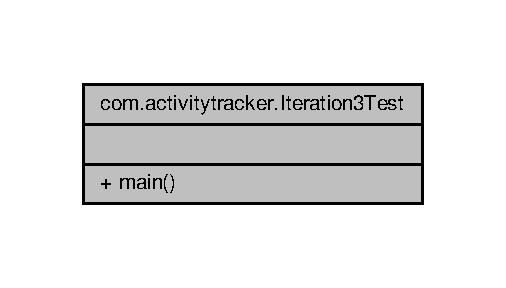
\includegraphics[width=241pt]{classcom_1_1activitytracker_1_1_iteration3_test__coll__graph}
\end{center}
\end{figure}
\subsection*{Static Public Member Functions}
\begin{DoxyCompactItemize}
\item 
static void \mbox{\hyperlink{classcom_1_1activitytracker_1_1_iteration3_test_a54f41d79b383667b8f79258dbfd7771c}{main}} (String\mbox{[}$\,$\mbox{]} args)
\end{DoxyCompactItemize}


\subsection{Detailed Description}


Definition at line 12 of file Iteration3\+Test.\+java.



\subsection{Member Function Documentation}
\mbox{\Hypertarget{classcom_1_1activitytracker_1_1_iteration3_test_a54f41d79b383667b8f79258dbfd7771c}\label{classcom_1_1activitytracker_1_1_iteration3_test_a54f41d79b383667b8f79258dbfd7771c}} 
\index{com\+::activitytracker\+::\+Iteration3\+Test@{com\+::activitytracker\+::\+Iteration3\+Test}!main@{main}}
\index{main@{main}!com\+::activitytracker\+::\+Iteration3\+Test@{com\+::activitytracker\+::\+Iteration3\+Test}}
\subsubsection{\texorpdfstring{main()}{main()}}
{\footnotesize\ttfamily static void com.\+activitytracker.\+Iteration3\+Test.\+main (\begin{DoxyParamCaption}\item[{String \mbox{[}$\,$\mbox{]}}]{args }\end{DoxyParamCaption})\hspace{0.3cm}{\ttfamily [static]}}



Definition at line 14 of file Iteration3\+Test.\+java.


\begin{DoxyCode}
14                                            \{
15 
16         \textcolor{comment}{// Iteration 1 begins here}
17 
18         User john = null;
19 
20         DBManager dbManager = \textcolor{keyword}{new} DBManager();
21         \textcolor{keywordflow}{if} (!dbManager.init(\textcolor{stringliteral}{"data.db"})) \{
22             System.err.println(\textcolor{stringliteral}{"Failed to initialize DBManager"});
23             System.exit(1);
24         \}
25 
26         System.out.println(\textcolor{stringliteral}{"Attempting to create user..."});
27 
28         \textcolor{keywordflow}{if} (!dbManager.userExists(\textcolor{stringliteral}{"jdoe@mac.com"}))
29             User.createUser(
30                     dbManager,
31                     \textcolor{stringliteral}{"John Doe"},
32                     \textcolor{stringliteral}{"jdoe@mac.com"},
33                     1997,
34                     12,
35                     12,
36                     User.Sex.MALE,
37                     1.6764f,
38                     54.4310844f,
39                     \textcolor{stringliteral}{"My Very Secure Password"}
40             );
41         \textcolor{keywordflow}{else}
42             System.out.println(\textcolor{stringliteral}{"User already exists."});
43 
44 
45 
46         \textcolor{keywordflow}{if} (dbManager.userExists(\textcolor{stringliteral}{"jdoe@mac.com"}))
47             System.out.println(\textcolor{stringliteral}{"John Doe was created!"});
48         \textcolor{keywordflow}{else}
49             System.out.println(\textcolor{stringliteral}{"User was NOT created."});
50 
51 
52         System.out.println(\textcolor{stringliteral}{"Testing incorrect password..."});
53 
54         \textcolor{keywordflow}{try} \{
55             john = \textcolor{keyword}{new} User(dbManager,\textcolor{stringliteral}{"jdoe@mac.com"}, \textcolor{stringliteral}{"Some Incorrect Password"});
56         \}
57         \textcolor{keywordflow}{catch} (\textcolor{keyword}{final} AuthenticationException e) \{
58             System.out.println(\textcolor{stringliteral}{"Incorrect password used; authentication failed."});
59         \}
60 
61         System.out.println(\textcolor{stringliteral}{"Authenticating user..."});
62 
63         \textcolor{keywordflow}{try} \{
64             john = \textcolor{keyword}{new} User(dbManager,\textcolor{stringliteral}{"jdoe@mac.com"}, \textcolor{stringliteral}{"My Very Secure Password"});
65         \}
66         \textcolor{keywordflow}{catch} (\textcolor{keyword}{final} AuthenticationException e) \{
67             System.out.println(\textcolor{stringliteral}{"Test failed; user could not be authenticated."});
68         \}
69 
70         \textcolor{comment}{// Iteration 1 ended here}
71 
72         \textcolor{comment}{// Iteration 2 begins here}
73 
74         \textcolor{keywordflow}{if} (john !=  null) \{
75             Date today = \textcolor{keyword}{new} Date();
76             \textcolor{keywordflow}{try} \{
77                 Run.bulkImport(dbManager, john, \textcolor{stringliteral}{"/Users/jacobhouse/Google Drive File Stream/My
       Drive/Documents/Courses/Computer Science/COMP-2005 Software Engineering/Final
       Project/comp2005-activity-tracker/app/InputWO.csv"});
78             \}
79             \textcolor{keywordflow}{catch} (\textcolor{keyword}{final} IOException e) \{
80                 System.err.println(e.getMessage());
81             \}
82         \}
83         \textcolor{keywordflow}{else} \{
84             System.out.println(\textcolor{stringliteral}{"John is null. Cannot execute phase 2."});
85         \}
86 
87         \textcolor{comment}{// Iteration 2 ends here}
88         \textcolor{comment}{// Iteration 3 begins here}
89 
90         Date date = null;
91         DateFormat sourceFormat = \textcolor{keyword}{new} SimpleDateFormat(\textcolor{stringliteral}{"dd-MM-yyyy"});
92 
93         \textcolor{keywordflow}{try} \{
94             date = sourceFormat.parse(\textcolor{stringliteral}{"01-01-2018"});
95         \}
96         \textcolor{keywordflow}{catch} (\textcolor{keyword}{final} ParseException e) \{
97             System.err.println(e.getMessage());
98         \}
99 
100         Vector<Run> runs = Run.getRuns(dbManager, john, date, \textcolor{keyword}{new} Date());
101 
102         \textcolor{keywordflow}{if} (runs == null) \{
103             System.out.println(\textcolor{stringliteral}{"Runs is null."});
104         \} \textcolor{keywordflow}{else} \textcolor{keywordflow}{if} (runs.size() == 0)
105             System.err.println(\textcolor{stringliteral}{"No runs in vector."});
106         \textcolor{keywordflow}{else}
107             \textcolor{keywordflow}{for} (Run run : runs) \{
108                 System.out.println(\textcolor{stringliteral}{"Retrieved run with ID "} + Integer.toString(run.getID()));
109             \}
110 
111 
112         \textcolor{comment}{// Iteration 3 ends here}
113 
114     \}
\end{DoxyCode}


The documentation for this class was generated from the following file\+:\begin{DoxyCompactItemize}
\item 
app/src/com/activitytracker/\mbox{\hyperlink{_iteration3_test_8java}{Iteration3\+Test.\+java}}\end{DoxyCompactItemize}

\hypertarget{classcom_1_1activitytracker_1_1_login_window}{}\section{com.\+activitytracker.\+Login\+Window Class Reference}
\label{classcom_1_1activitytracker_1_1_login_window}\index{com.\+activitytracker.\+Login\+Window@{com.\+activitytracker.\+Login\+Window}}


Inheritance diagram for com.\+activitytracker.\+Login\+Window\+:
\nopagebreak
\begin{figure}[H]
\begin{center}
\leavevmode
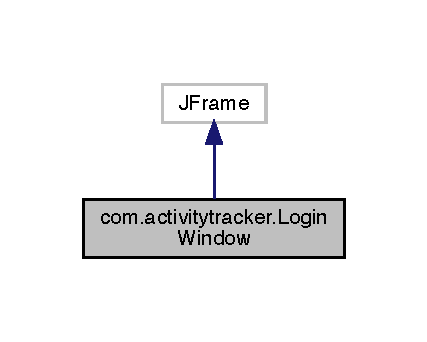
\includegraphics[width=213pt]{classcom_1_1activitytracker_1_1_login_window__inherit__graph}
\end{center}
\end{figure}


Collaboration diagram for com.\+activitytracker.\+Login\+Window\+:
\nopagebreak
\begin{figure}[H]
\begin{center}
\leavevmode
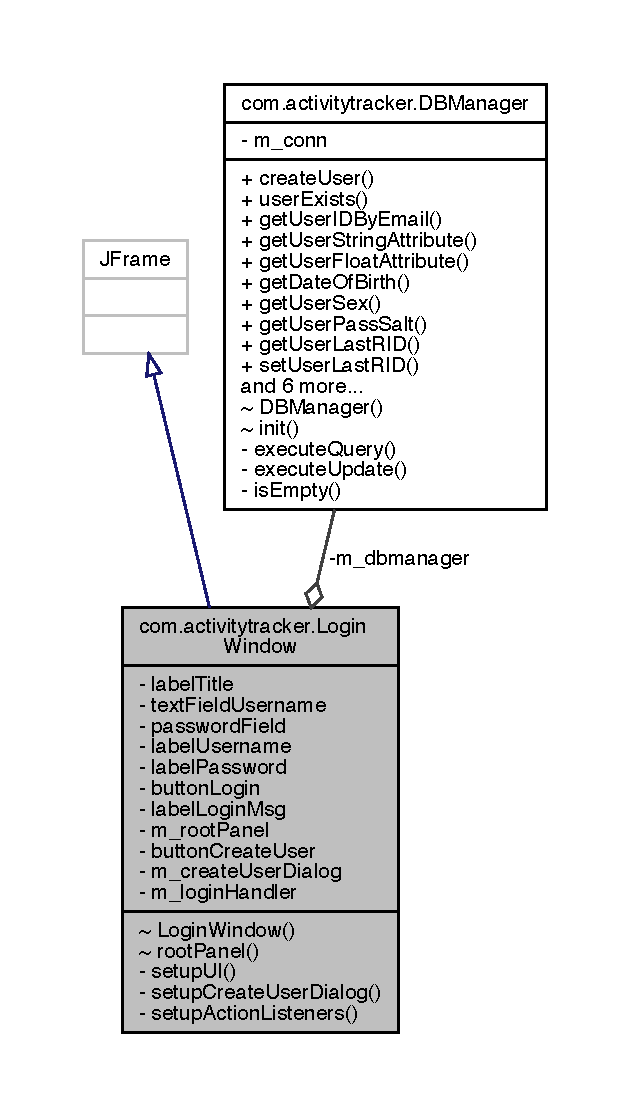
\includegraphics[width=213pt]{classcom_1_1activitytracker_1_1_login_window__coll__graph}
\end{center}
\end{figure}
\subsection*{Package Functions}
\begin{DoxyCompactItemize}
\item 
\mbox{\hyperlink{classcom_1_1activitytracker_1_1_login_window_a137cce127ffa1660c70d3fddbc0e2a74}{Login\+Window}} (java.\+util.\+function.\+Consumer$<$ Void $>$ login\+Handler)
\item 
J\+Panel \mbox{\hyperlink{classcom_1_1activitytracker_1_1_login_window_ab1ea45e86bbb79bccd06531279f1e443}{root\+Panel}} ()
\end{DoxyCompactItemize}
\subsection*{Private Member Functions}
\begin{DoxyCompactItemize}
\item 
void \mbox{\hyperlink{classcom_1_1activitytracker_1_1_login_window_a7af9edf52b3028437e2159f0be9893a9}{setup\+UI}} ()
\item 
void \mbox{\hyperlink{classcom_1_1activitytracker_1_1_login_window_a567db7b15448fe9d9c76addbcee4092b}{setup\+Create\+User\+Dialog}} ()
\item 
void \mbox{\hyperlink{classcom_1_1activitytracker_1_1_login_window_af1ff236b841c51bfb49e143344a3c3ac}{setup\+Action\+Listeners}} ()
\end{DoxyCompactItemize}
\subsection*{Private Attributes}
\begin{DoxyCompactItemize}
\item 
J\+Label \mbox{\hyperlink{classcom_1_1activitytracker_1_1_login_window_a3c4c84a656351094b34320a5c352e685}{label\+Title}}
\item 
J\+Text\+Field \mbox{\hyperlink{classcom_1_1activitytracker_1_1_login_window_aba181dcec114c349a67304406bcce92a}{text\+Field\+Username}}
\item 
J\+Password\+Field \mbox{\hyperlink{classcom_1_1activitytracker_1_1_login_window_ae53353ceea197fe7b93f1b7156112d08}{password\+Field}}
\item 
J\+Label \mbox{\hyperlink{classcom_1_1activitytracker_1_1_login_window_a4999e1461716e42ee4e3de8e3eb47eb9}{label\+Username}}
\item 
J\+Label \mbox{\hyperlink{classcom_1_1activitytracker_1_1_login_window_a8be41422fca8038bd8c2ba49af8ae6ce}{label\+Password}}
\item 
J\+Button \mbox{\hyperlink{classcom_1_1activitytracker_1_1_login_window_ac77d9f8f3a6c697a9847ecd130ac2ef6}{button\+Login}}
\item 
J\+Label \mbox{\hyperlink{classcom_1_1activitytracker_1_1_login_window_a567ae49b39c07840b39eec92fdf92c22}{label\+Login\+Msg}}
\item 
J\+Panel \mbox{\hyperlink{classcom_1_1activitytracker_1_1_login_window_aa62049382baddb801cb25201814efc57}{m\+\_\+root\+Panel}}
\item 
J\+Button \mbox{\hyperlink{classcom_1_1activitytracker_1_1_login_window_a1ff77d6846d01d4a8540371ede091371}{button\+Create\+User}}
\item 
J\+Dialog \mbox{\hyperlink{classcom_1_1activitytracker_1_1_login_window_a49ff7093e29ce7bd22c42ac8099d5d34}{m\+\_\+create\+User\+Dialog}} = null
\item 
java.\+util.\+function.\+Consumer$<$ Void $>$ \mbox{\hyperlink{classcom_1_1activitytracker_1_1_login_window_aab28a8e6372499a8690d524dedeaf9e1}{m\+\_\+login\+Handler}}
\end{DoxyCompactItemize}


\subsection{Detailed Description}


Definition at line 11 of file Login\+Window.\+java.



\subsection{Constructor \& Destructor Documentation}
\mbox{\Hypertarget{classcom_1_1activitytracker_1_1_login_window_a137cce127ffa1660c70d3fddbc0e2a74}\label{classcom_1_1activitytracker_1_1_login_window_a137cce127ffa1660c70d3fddbc0e2a74}} 
\index{com\+::activitytracker\+::\+Login\+Window@{com\+::activitytracker\+::\+Login\+Window}!Login\+Window@{Login\+Window}}
\index{Login\+Window@{Login\+Window}!com\+::activitytracker\+::\+Login\+Window@{com\+::activitytracker\+::\+Login\+Window}}
\subsubsection{\texorpdfstring{Login\+Window()}{LoginWindow()}}
{\footnotesize\ttfamily com.\+activitytracker.\+Login\+Window.\+Login\+Window (\begin{DoxyParamCaption}\item[{java.\+util.\+function.\+Consumer$<$ Void $>$}]{login\+Handler }\end{DoxyParamCaption})\hspace{0.3cm}{\ttfamily [package]}}



Definition at line 26 of file Login\+Window.\+java.


\begin{DoxyCode}
26                                                                 \{
27         \mbox{\hyperlink{classcom_1_1activitytracker_1_1_login_window_aab28a8e6372499a8690d524dedeaf9e1}{m\_loginHandler}} = loginHandler;
28 
29         \mbox{\hyperlink{classcom_1_1activitytracker_1_1_login_window_a7af9edf52b3028437e2159f0be9893a9}{setupUI}}();
30         \mbox{\hyperlink{classcom_1_1activitytracker_1_1_login_window_a567db7b15448fe9d9c76addbcee4092b}{setupCreateUserDialog}}();
31         \mbox{\hyperlink{classcom_1_1activitytracker_1_1_login_window_af1ff236b841c51bfb49e143344a3c3ac}{setupActionListeners}}();
32     \}
\end{DoxyCode}


\subsection{Member Function Documentation}
\mbox{\Hypertarget{classcom_1_1activitytracker_1_1_login_window_ab1ea45e86bbb79bccd06531279f1e443}\label{classcom_1_1activitytracker_1_1_login_window_ab1ea45e86bbb79bccd06531279f1e443}} 
\index{com\+::activitytracker\+::\+Login\+Window@{com\+::activitytracker\+::\+Login\+Window}!root\+Panel@{root\+Panel}}
\index{root\+Panel@{root\+Panel}!com\+::activitytracker\+::\+Login\+Window@{com\+::activitytracker\+::\+Login\+Window}}
\subsubsection{\texorpdfstring{root\+Panel()}{rootPanel()}}
{\footnotesize\ttfamily J\+Panel com.\+activitytracker.\+Login\+Window.\+root\+Panel (\begin{DoxyParamCaption}{ }\end{DoxyParamCaption})\hspace{0.3cm}{\ttfamily [package]}}



Definition at line 85 of file Login\+Window.\+java.


\begin{DoxyCode}
85                        \{
86         \textcolor{keywordflow}{return} \mbox{\hyperlink{classcom_1_1activitytracker_1_1_login_window_aa62049382baddb801cb25201814efc57}{m\_rootPanel}};
87     \}
\end{DoxyCode}
\mbox{\Hypertarget{classcom_1_1activitytracker_1_1_login_window_af1ff236b841c51bfb49e143344a3c3ac}\label{classcom_1_1activitytracker_1_1_login_window_af1ff236b841c51bfb49e143344a3c3ac}} 
\index{com\+::activitytracker\+::\+Login\+Window@{com\+::activitytracker\+::\+Login\+Window}!setup\+Action\+Listeners@{setup\+Action\+Listeners}}
\index{setup\+Action\+Listeners@{setup\+Action\+Listeners}!com\+::activitytracker\+::\+Login\+Window@{com\+::activitytracker\+::\+Login\+Window}}
\subsubsection{\texorpdfstring{setup\+Action\+Listeners()}{setupActionListeners()}}
{\footnotesize\ttfamily void com.\+activitytracker.\+Login\+Window.\+setup\+Action\+Listeners (\begin{DoxyParamCaption}{ }\end{DoxyParamCaption})\hspace{0.3cm}{\ttfamily [private]}}



Definition at line 54 of file Login\+Window.\+java.


\begin{DoxyCode}
54                                         \{
55 
56         \textcolor{comment}{// Login button}
57         \mbox{\hyperlink{classcom_1_1activitytracker_1_1_login_window_ac77d9f8f3a6c697a9847ecd130ac2ef6}{buttonLogin}}.addActionListener(\textcolor{keyword}{new} ActionListener() \{
58             @Override
59             \textcolor{keyword}{public} \textcolor{keywordtype}{void} actionPerformed(ActionEvent e) \{
60 
61                 \textcolor{comment}{// Do nothing if login fields are empty}
62                 \textcolor{keywordflow}{if} (\mbox{\hyperlink{classcom_1_1activitytracker_1_1_login_window_aba181dcec114c349a67304406bcce92a}{textFieldUsername}}.getText().isEmpty() || 
      \mbox{\hyperlink{classcom_1_1activitytracker_1_1_login_window_ae53353ceea197fe7b93f1b7156112d08}{passwordField}}.getPassword().length == 0) \{
63                     \textcolor{keywordflow}{return};
64                 \}
65 
66                 \textcolor{comment}{// Change to verifyLogin()}
67                 \textcolor{keywordflow}{if} (\textcolor{keyword}{true}) \{
68                     \mbox{\hyperlink{classcom_1_1activitytracker_1_1_login_window_aab28a8e6372499a8690d524dedeaf9e1}{m\_loginHandler}}.accept(null);
69                     \textcolor{keywordflow}{return};
70                 \}
71 
72                 \textcolor{comment}{// Display error message}
73             \}
74         \});
75 
76         \textcolor{comment}{// Create user button}
77         \mbox{\hyperlink{classcom_1_1activitytracker_1_1_login_window_a1ff77d6846d01d4a8540371ede091371}{buttonCreateUser}}.addActionListener(\textcolor{keyword}{new} ActionListener() \{
78             @Override
79             \textcolor{keyword}{public} \textcolor{keywordtype}{void} actionPerformed(ActionEvent e) \{
80                 \mbox{\hyperlink{classcom_1_1activitytracker_1_1_login_window_a49ff7093e29ce7bd22c42ac8099d5d34}{m\_createUserDialog}}.setVisible(\textcolor{keyword}{true});
81             \}
82         \});
83     \}
\end{DoxyCode}
\mbox{\Hypertarget{classcom_1_1activitytracker_1_1_login_window_a567db7b15448fe9d9c76addbcee4092b}\label{classcom_1_1activitytracker_1_1_login_window_a567db7b15448fe9d9c76addbcee4092b}} 
\index{com\+::activitytracker\+::\+Login\+Window@{com\+::activitytracker\+::\+Login\+Window}!setup\+Create\+User\+Dialog@{setup\+Create\+User\+Dialog}}
\index{setup\+Create\+User\+Dialog@{setup\+Create\+User\+Dialog}!com\+::activitytracker\+::\+Login\+Window@{com\+::activitytracker\+::\+Login\+Window}}
\subsubsection{\texorpdfstring{setup\+Create\+User\+Dialog()}{setupCreateUserDialog()}}
{\footnotesize\ttfamily void com.\+activitytracker.\+Login\+Window.\+setup\+Create\+User\+Dialog (\begin{DoxyParamCaption}{ }\end{DoxyParamCaption})\hspace{0.3cm}{\ttfamily [private]}}



Definition at line 41 of file Login\+Window.\+java.


\begin{DoxyCode}
41                                          \{
42 
43         \textcolor{comment}{// Get desktop resolution of default monitor (in case of multi-monitor setups)}
44         \textcolor{keyword}{final} GraphicsDevice gd = GraphicsEnvironment.getLocalGraphicsEnvironment().getDefaultScreenDevice(
      );
45 
46         \mbox{\hyperlink{classcom_1_1activitytracker_1_1_login_window_a49ff7093e29ce7bd22c42ac8099d5d34}{m\_createUserDialog}} = \textcolor{keyword}{new} JDialog(\textcolor{keyword}{this}, \textcolor{stringliteral}{"Activity Logger | Create User"}, \textcolor{keyword}{true});
47         \mbox{\hyperlink{classcom_1_1activitytracker_1_1_login_window_a49ff7093e29ce7bd22c42ac8099d5d34}{m\_createUserDialog}}.setContentPane(\textcolor{keyword}{new} CreateUserWindow().
      \mbox{\hyperlink{classcom_1_1activitytracker_1_1_login_window_ab1ea45e86bbb79bccd06531279f1e443}{rootPanel}}());
48         \mbox{\hyperlink{classcom_1_1activitytracker_1_1_login_window_a49ff7093e29ce7bd22c42ac8099d5d34}{m\_createUserDialog}}.pack();
49         \textcolor{comment}{// Set window size to be 1/2 of screen dimensions}
50         \mbox{\hyperlink{classcom_1_1activitytracker_1_1_login_window_a49ff7093e29ce7bd22c42ac8099d5d34}{m\_createUserDialog}}.setSize(gd.getDisplayMode().getWidth() / 2, gd.getDisplayMode(
      ).getHeight() / 2);
51         \mbox{\hyperlink{classcom_1_1activitytracker_1_1_login_window_a49ff7093e29ce7bd22c42ac8099d5d34}{m\_createUserDialog}}.setLocationRelativeTo(\textcolor{keyword}{this}); \textcolor{comment}{// Center window}
52     \}
\end{DoxyCode}
\mbox{\Hypertarget{classcom_1_1activitytracker_1_1_login_window_a7af9edf52b3028437e2159f0be9893a9}\label{classcom_1_1activitytracker_1_1_login_window_a7af9edf52b3028437e2159f0be9893a9}} 
\index{com\+::activitytracker\+::\+Login\+Window@{com\+::activitytracker\+::\+Login\+Window}!setup\+UI@{setup\+UI}}
\index{setup\+UI@{setup\+UI}!com\+::activitytracker\+::\+Login\+Window@{com\+::activitytracker\+::\+Login\+Window}}
\subsubsection{\texorpdfstring{setup\+U\+I()}{setupUI()}}
{\footnotesize\ttfamily void com.\+activitytracker.\+Login\+Window.\+setup\+UI (\begin{DoxyParamCaption}{ }\end{DoxyParamCaption})\hspace{0.3cm}{\ttfamily [private]}}



Definition at line 34 of file Login\+Window.\+java.


\begin{DoxyCode}
34                            \{
35         MaterialUIMovement.add(\mbox{\hyperlink{classcom_1_1activitytracker_1_1_login_window_ac77d9f8f3a6c697a9847ecd130ac2ef6}{buttonLogin}}, MaterialColors.GRAY\_100);
36         MaterialUIMovement.add(\mbox{\hyperlink{classcom_1_1activitytracker_1_1_login_window_a1ff77d6846d01d4a8540371ede091371}{buttonCreateUser}}, MaterialColors.GRAY\_100);
37 
38         \mbox{\hyperlink{classcom_1_1activitytracker_1_1_login_window_a567ae49b39c07840b39eec92fdf92c22}{labelLoginMsg}}.setVisible(\textcolor{keyword}{false});
39     \}
\end{DoxyCode}


\subsection{Member Data Documentation}
\mbox{\Hypertarget{classcom_1_1activitytracker_1_1_login_window_a1ff77d6846d01d4a8540371ede091371}\label{classcom_1_1activitytracker_1_1_login_window_a1ff77d6846d01d4a8540371ede091371}} 
\index{com\+::activitytracker\+::\+Login\+Window@{com\+::activitytracker\+::\+Login\+Window}!button\+Create\+User@{button\+Create\+User}}
\index{button\+Create\+User@{button\+Create\+User}!com\+::activitytracker\+::\+Login\+Window@{com\+::activitytracker\+::\+Login\+Window}}
\subsubsection{\texorpdfstring{button\+Create\+User}{buttonCreateUser}}
{\footnotesize\ttfamily J\+Button com.\+activitytracker.\+Login\+Window.\+button\+Create\+User\hspace{0.3cm}{\ttfamily [private]}}



Definition at line 20 of file Login\+Window.\+java.

\mbox{\Hypertarget{classcom_1_1activitytracker_1_1_login_window_ac77d9f8f3a6c697a9847ecd130ac2ef6}\label{classcom_1_1activitytracker_1_1_login_window_ac77d9f8f3a6c697a9847ecd130ac2ef6}} 
\index{com\+::activitytracker\+::\+Login\+Window@{com\+::activitytracker\+::\+Login\+Window}!button\+Login@{button\+Login}}
\index{button\+Login@{button\+Login}!com\+::activitytracker\+::\+Login\+Window@{com\+::activitytracker\+::\+Login\+Window}}
\subsubsection{\texorpdfstring{button\+Login}{buttonLogin}}
{\footnotesize\ttfamily J\+Button com.\+activitytracker.\+Login\+Window.\+button\+Login\hspace{0.3cm}{\ttfamily [private]}}



Definition at line 17 of file Login\+Window.\+java.

\mbox{\Hypertarget{classcom_1_1activitytracker_1_1_login_window_a567ae49b39c07840b39eec92fdf92c22}\label{classcom_1_1activitytracker_1_1_login_window_a567ae49b39c07840b39eec92fdf92c22}} 
\index{com\+::activitytracker\+::\+Login\+Window@{com\+::activitytracker\+::\+Login\+Window}!label\+Login\+Msg@{label\+Login\+Msg}}
\index{label\+Login\+Msg@{label\+Login\+Msg}!com\+::activitytracker\+::\+Login\+Window@{com\+::activitytracker\+::\+Login\+Window}}
\subsubsection{\texorpdfstring{label\+Login\+Msg}{labelLoginMsg}}
{\footnotesize\ttfamily J\+Label com.\+activitytracker.\+Login\+Window.\+label\+Login\+Msg\hspace{0.3cm}{\ttfamily [private]}}



Definition at line 18 of file Login\+Window.\+java.

\mbox{\Hypertarget{classcom_1_1activitytracker_1_1_login_window_a8be41422fca8038bd8c2ba49af8ae6ce}\label{classcom_1_1activitytracker_1_1_login_window_a8be41422fca8038bd8c2ba49af8ae6ce}} 
\index{com\+::activitytracker\+::\+Login\+Window@{com\+::activitytracker\+::\+Login\+Window}!label\+Password@{label\+Password}}
\index{label\+Password@{label\+Password}!com\+::activitytracker\+::\+Login\+Window@{com\+::activitytracker\+::\+Login\+Window}}
\subsubsection{\texorpdfstring{label\+Password}{labelPassword}}
{\footnotesize\ttfamily J\+Label com.\+activitytracker.\+Login\+Window.\+label\+Password\hspace{0.3cm}{\ttfamily [private]}}



Definition at line 16 of file Login\+Window.\+java.

\mbox{\Hypertarget{classcom_1_1activitytracker_1_1_login_window_a3c4c84a656351094b34320a5c352e685}\label{classcom_1_1activitytracker_1_1_login_window_a3c4c84a656351094b34320a5c352e685}} 
\index{com\+::activitytracker\+::\+Login\+Window@{com\+::activitytracker\+::\+Login\+Window}!label\+Title@{label\+Title}}
\index{label\+Title@{label\+Title}!com\+::activitytracker\+::\+Login\+Window@{com\+::activitytracker\+::\+Login\+Window}}
\subsubsection{\texorpdfstring{label\+Title}{labelTitle}}
{\footnotesize\ttfamily J\+Label com.\+activitytracker.\+Login\+Window.\+label\+Title\hspace{0.3cm}{\ttfamily [private]}}



Definition at line 12 of file Login\+Window.\+java.

\mbox{\Hypertarget{classcom_1_1activitytracker_1_1_login_window_a4999e1461716e42ee4e3de8e3eb47eb9}\label{classcom_1_1activitytracker_1_1_login_window_a4999e1461716e42ee4e3de8e3eb47eb9}} 
\index{com\+::activitytracker\+::\+Login\+Window@{com\+::activitytracker\+::\+Login\+Window}!label\+Username@{label\+Username}}
\index{label\+Username@{label\+Username}!com\+::activitytracker\+::\+Login\+Window@{com\+::activitytracker\+::\+Login\+Window}}
\subsubsection{\texorpdfstring{label\+Username}{labelUsername}}
{\footnotesize\ttfamily J\+Label com.\+activitytracker.\+Login\+Window.\+label\+Username\hspace{0.3cm}{\ttfamily [private]}}



Definition at line 15 of file Login\+Window.\+java.

\mbox{\Hypertarget{classcom_1_1activitytracker_1_1_login_window_a49ff7093e29ce7bd22c42ac8099d5d34}\label{classcom_1_1activitytracker_1_1_login_window_a49ff7093e29ce7bd22c42ac8099d5d34}} 
\index{com\+::activitytracker\+::\+Login\+Window@{com\+::activitytracker\+::\+Login\+Window}!m\+\_\+create\+User\+Dialog@{m\+\_\+create\+User\+Dialog}}
\index{m\+\_\+create\+User\+Dialog@{m\+\_\+create\+User\+Dialog}!com\+::activitytracker\+::\+Login\+Window@{com\+::activitytracker\+::\+Login\+Window}}
\subsubsection{\texorpdfstring{m\+\_\+create\+User\+Dialog}{m\_createUserDialog}}
{\footnotesize\ttfamily J\+Dialog com.\+activitytracker.\+Login\+Window.\+m\+\_\+create\+User\+Dialog = null\hspace{0.3cm}{\ttfamily [private]}}



Definition at line 22 of file Login\+Window.\+java.

\mbox{\Hypertarget{classcom_1_1activitytracker_1_1_login_window_aab28a8e6372499a8690d524dedeaf9e1}\label{classcom_1_1activitytracker_1_1_login_window_aab28a8e6372499a8690d524dedeaf9e1}} 
\index{com\+::activitytracker\+::\+Login\+Window@{com\+::activitytracker\+::\+Login\+Window}!m\+\_\+login\+Handler@{m\+\_\+login\+Handler}}
\index{m\+\_\+login\+Handler@{m\+\_\+login\+Handler}!com\+::activitytracker\+::\+Login\+Window@{com\+::activitytracker\+::\+Login\+Window}}
\subsubsection{\texorpdfstring{m\+\_\+login\+Handler}{m\_loginHandler}}
{\footnotesize\ttfamily java.\+util.\+function.\+Consumer$<$Void$>$ com.\+activitytracker.\+Login\+Window.\+m\+\_\+login\+Handler\hspace{0.3cm}{\ttfamily [private]}}



Definition at line 24 of file Login\+Window.\+java.

\mbox{\Hypertarget{classcom_1_1activitytracker_1_1_login_window_aa62049382baddb801cb25201814efc57}\label{classcom_1_1activitytracker_1_1_login_window_aa62049382baddb801cb25201814efc57}} 
\index{com\+::activitytracker\+::\+Login\+Window@{com\+::activitytracker\+::\+Login\+Window}!m\+\_\+root\+Panel@{m\+\_\+root\+Panel}}
\index{m\+\_\+root\+Panel@{m\+\_\+root\+Panel}!com\+::activitytracker\+::\+Login\+Window@{com\+::activitytracker\+::\+Login\+Window}}
\subsubsection{\texorpdfstring{m\+\_\+root\+Panel}{m\_rootPanel}}
{\footnotesize\ttfamily J\+Panel com.\+activitytracker.\+Login\+Window.\+m\+\_\+root\+Panel\hspace{0.3cm}{\ttfamily [private]}}



Definition at line 19 of file Login\+Window.\+java.

\mbox{\Hypertarget{classcom_1_1activitytracker_1_1_login_window_ae53353ceea197fe7b93f1b7156112d08}\label{classcom_1_1activitytracker_1_1_login_window_ae53353ceea197fe7b93f1b7156112d08}} 
\index{com\+::activitytracker\+::\+Login\+Window@{com\+::activitytracker\+::\+Login\+Window}!password\+Field@{password\+Field}}
\index{password\+Field@{password\+Field}!com\+::activitytracker\+::\+Login\+Window@{com\+::activitytracker\+::\+Login\+Window}}
\subsubsection{\texorpdfstring{password\+Field}{passwordField}}
{\footnotesize\ttfamily J\+Password\+Field com.\+activitytracker.\+Login\+Window.\+password\+Field\hspace{0.3cm}{\ttfamily [private]}}



Definition at line 14 of file Login\+Window.\+java.

\mbox{\Hypertarget{classcom_1_1activitytracker_1_1_login_window_aba181dcec114c349a67304406bcce92a}\label{classcom_1_1activitytracker_1_1_login_window_aba181dcec114c349a67304406bcce92a}} 
\index{com\+::activitytracker\+::\+Login\+Window@{com\+::activitytracker\+::\+Login\+Window}!text\+Field\+Username@{text\+Field\+Username}}
\index{text\+Field\+Username@{text\+Field\+Username}!com\+::activitytracker\+::\+Login\+Window@{com\+::activitytracker\+::\+Login\+Window}}
\subsubsection{\texorpdfstring{text\+Field\+Username}{textFieldUsername}}
{\footnotesize\ttfamily J\+Text\+Field com.\+activitytracker.\+Login\+Window.\+text\+Field\+Username\hspace{0.3cm}{\ttfamily [private]}}



Definition at line 13 of file Login\+Window.\+java.



The documentation for this class was generated from the following file\+:\begin{DoxyCompactItemize}
\item 
app/src/com/activitytracker/\mbox{\hyperlink{_login_window_8java}{Login\+Window.\+java}}\end{DoxyCompactItemize}

\hypertarget{classcom_1_1activitytracker_1_1_main_window}{}\section{com.\+activitytracker.\+Main\+Window Class Reference}
\label{classcom_1_1activitytracker_1_1_main_window}\index{com.\+activitytracker.\+Main\+Window@{com.\+activitytracker.\+Main\+Window}}
\subsection*{Package Functions}
\begin{DoxyCompactItemize}
\item 
\mbox{\hyperlink{classcom_1_1activitytracker_1_1_main_window_a77d0ebef154786202a165f496dc70065}{Main\+Window}} ()
\item 
J\+Panel \mbox{\hyperlink{classcom_1_1activitytracker_1_1_main_window_a62e9c6f477ccc5b93aff33abb567fde4}{root\+Panel}} ()
\end{DoxyCompactItemize}
\subsection*{Private Member Functions}
\begin{DoxyCompactItemize}
\item 
void \mbox{\hyperlink{classcom_1_1activitytracker_1_1_main_window_a53a019623a37b950473359fc625b6423}{setup\+UI}} ()
\item 
void \mbox{\hyperlink{classcom_1_1activitytracker_1_1_main_window_a76b3e8567b228ccd26f09c15ebaddb72}{setup\+Action\+Listeners}} ()
\end{DoxyCompactItemize}
\subsection*{Private Attributes}
\begin{DoxyCompactItemize}
\item 
J\+Panel \mbox{\hyperlink{classcom_1_1activitytracker_1_1_main_window_ac3d61c032aef87f12b1ae6f7dbf482c3}{m\+\_\+root\+Panel}}
\item 
J\+Panel \mbox{\hyperlink{classcom_1_1activitytracker_1_1_main_window_a6baf76b2b8ede1ba82fc6d096ddb580b}{top\+Panel}}
\item 
J\+Button \mbox{\hyperlink{classcom_1_1activitytracker_1_1_main_window_adec15801f8e16f769bd954e351a663fa}{button\+My\+Activity}}
\item 
J\+Button \mbox{\hyperlink{classcom_1_1activitytracker_1_1_main_window_af241d0ee8023ed099caa204419d74ccb}{button\+Add\+Device}}
\item 
J\+Button \mbox{\hyperlink{classcom_1_1activitytracker_1_1_main_window_a4d9543db1723fd7d1921f07cc92e2abb}{button\+My\+Friends}}
\item 
J\+Panel \mbox{\hyperlink{classcom_1_1activitytracker_1_1_main_window_aaa5ce3b10bff65231c65a3d4b33724b0}{content\+Panel}}
\item 
J\+Label \mbox{\hyperlink{classcom_1_1activitytracker_1_1_main_window_a05a555ba49d30b00573d07e5acd39e0a}{label\+Profile\+Icon}}
\item 
J\+Panel \mbox{\hyperlink{classcom_1_1activitytracker_1_1_main_window_a89833c824727a496f4a889177d4d3f3c}{panel\+My\+Activity}}
\item 
J\+Panel \mbox{\hyperlink{classcom_1_1activitytracker_1_1_main_window_a02f203d3c00a61d838fcee4657984584}{panel\+Add\+Device}}
\item 
J\+Panel \mbox{\hyperlink{classcom_1_1activitytracker_1_1_main_window_afc5efa70337b4b072b38c2cc30991473}{panel\+My\+Friends}}
\item 
J\+Scroll\+Pane \mbox{\hyperlink{classcom_1_1activitytracker_1_1_main_window_a4ef571b624e78e91f3ccad9234c0b5d3}{scroll\+Pane\+My\+Friends}}
\item 
J\+Table \mbox{\hyperlink{classcom_1_1activitytracker_1_1_main_window_a50012386053e035e7ae0fb993153b225}{table\+Available\+Devices}}
\item 
J\+Table \mbox{\hyperlink{classcom_1_1activitytracker_1_1_main_window_a0ad6d3ca1298275eba15a9ea189d4d9b}{table\+My\+Activity}}
\end{DoxyCompactItemize}


\subsection{Detailed Description}


Definition at line 12 of file Main\+Window.\+java.



\subsection{Constructor \& Destructor Documentation}
\mbox{\Hypertarget{classcom_1_1activitytracker_1_1_main_window_a77d0ebef154786202a165f496dc70065}\label{classcom_1_1activitytracker_1_1_main_window_a77d0ebef154786202a165f496dc70065}} 
\index{com\+::activitytracker\+::\+Main\+Window@{com\+::activitytracker\+::\+Main\+Window}!Main\+Window@{Main\+Window}}
\index{Main\+Window@{Main\+Window}!com\+::activitytracker\+::\+Main\+Window@{com\+::activitytracker\+::\+Main\+Window}}
\subsubsection{\texorpdfstring{Main\+Window()}{MainWindow()}}
{\footnotesize\ttfamily com.\+activitytracker.\+Main\+Window.\+Main\+Window (\begin{DoxyParamCaption}{ }\end{DoxyParamCaption})\hspace{0.3cm}{\ttfamily [package]}}



Definition at line 27 of file Main\+Window.\+java.


\begin{DoxyCode}
27                  \{
28         \mbox{\hyperlink{classcom_1_1activitytracker_1_1_main_window_a53a019623a37b950473359fc625b6423}{setupUI}}();
29         \mbox{\hyperlink{classcom_1_1activitytracker_1_1_main_window_a76b3e8567b228ccd26f09c15ebaddb72}{setupActionListeners}}();
30     \}
\end{DoxyCode}


\subsection{Member Function Documentation}
\mbox{\Hypertarget{classcom_1_1activitytracker_1_1_main_window_a62e9c6f477ccc5b93aff33abb567fde4}\label{classcom_1_1activitytracker_1_1_main_window_a62e9c6f477ccc5b93aff33abb567fde4}} 
\index{com\+::activitytracker\+::\+Main\+Window@{com\+::activitytracker\+::\+Main\+Window}!root\+Panel@{root\+Panel}}
\index{root\+Panel@{root\+Panel}!com\+::activitytracker\+::\+Main\+Window@{com\+::activitytracker\+::\+Main\+Window}}
\subsubsection{\texorpdfstring{root\+Panel()}{rootPanel()}}
{\footnotesize\ttfamily J\+Panel com.\+activitytracker.\+Main\+Window.\+root\+Panel (\begin{DoxyParamCaption}{ }\end{DoxyParamCaption})\hspace{0.3cm}{\ttfamily [package]}}



Definition at line 84 of file Main\+Window.\+java.


\begin{DoxyCode}
84                        \{
85         \textcolor{keywordflow}{return} \mbox{\hyperlink{classcom_1_1activitytracker_1_1_main_window_ac3d61c032aef87f12b1ae6f7dbf482c3}{m\_rootPanel}};
86     \}
\end{DoxyCode}
\mbox{\Hypertarget{classcom_1_1activitytracker_1_1_main_window_a76b3e8567b228ccd26f09c15ebaddb72}\label{classcom_1_1activitytracker_1_1_main_window_a76b3e8567b228ccd26f09c15ebaddb72}} 
\index{com\+::activitytracker\+::\+Main\+Window@{com\+::activitytracker\+::\+Main\+Window}!setup\+Action\+Listeners@{setup\+Action\+Listeners}}
\index{setup\+Action\+Listeners@{setup\+Action\+Listeners}!com\+::activitytracker\+::\+Main\+Window@{com\+::activitytracker\+::\+Main\+Window}}
\subsubsection{\texorpdfstring{setup\+Action\+Listeners()}{setupActionListeners()}}
{\footnotesize\ttfamily void com.\+activitytracker.\+Main\+Window.\+setup\+Action\+Listeners (\begin{DoxyParamCaption}{ }\end{DoxyParamCaption})\hspace{0.3cm}{\ttfamily [private]}}



Definition at line 54 of file Main\+Window.\+java.


\begin{DoxyCode}
54                                         \{
55         \textcolor{comment}{// My Activity button}
56         \mbox{\hyperlink{classcom_1_1activitytracker_1_1_main_window_adec15801f8e16f769bd954e351a663fa}{buttonMyActivity}}.addActionListener(\textcolor{keyword}{new} ActionListener() \{
57             @Override
58             \textcolor{keyword}{public} \textcolor{keywordtype}{void} actionPerformed(ActionEvent actionEvent) \{
59                 \mbox{\hyperlink{classcom_1_1activitytracker_1_1_main_window_a89833c824727a496f4a889177d4d3f3c}{panelMyActivity}}.setVisible(\textcolor{keyword}{true});
60                 \mbox{\hyperlink{classcom_1_1activitytracker_1_1_main_window_a02f203d3c00a61d838fcee4657984584}{panelAddDevice}}.setVisible(\textcolor{keyword}{false});
61                 \mbox{\hyperlink{classcom_1_1activitytracker_1_1_main_window_afc5efa70337b4b072b38c2cc30991473}{panelMyFriends}}.setVisible(\textcolor{keyword}{false});
62             \}
63         \});
64         \textcolor{comment}{// Add Device button}
65         \mbox{\hyperlink{classcom_1_1activitytracker_1_1_main_window_af241d0ee8023ed099caa204419d74ccb}{buttonAddDevice}}.addActionListener(\textcolor{keyword}{new} ActionListener() \{
66             @Override
67             \textcolor{keyword}{public} \textcolor{keywordtype}{void} actionPerformed(ActionEvent actionEvent) \{
68                 \mbox{\hyperlink{classcom_1_1activitytracker_1_1_main_window_a89833c824727a496f4a889177d4d3f3c}{panelMyActivity}}.setVisible(\textcolor{keyword}{false});
69                 \mbox{\hyperlink{classcom_1_1activitytracker_1_1_main_window_a02f203d3c00a61d838fcee4657984584}{panelAddDevice}}.setVisible(\textcolor{keyword}{true});
70                 \mbox{\hyperlink{classcom_1_1activitytracker_1_1_main_window_afc5efa70337b4b072b38c2cc30991473}{panelMyFriends}}.setVisible(\textcolor{keyword}{false});
71             \}
72         \});
73         \textcolor{comment}{// My Friends button}
74         \mbox{\hyperlink{classcom_1_1activitytracker_1_1_main_window_a4d9543db1723fd7d1921f07cc92e2abb}{buttonMyFriends}}.addActionListener(\textcolor{keyword}{new} ActionListener() \{
75             @Override
76             \textcolor{keyword}{public} \textcolor{keywordtype}{void} actionPerformed(ActionEvent actionEvent) \{
77                 \mbox{\hyperlink{classcom_1_1activitytracker_1_1_main_window_a89833c824727a496f4a889177d4d3f3c}{panelMyActivity}}.setVisible(\textcolor{keyword}{false});
78                 \mbox{\hyperlink{classcom_1_1activitytracker_1_1_main_window_a02f203d3c00a61d838fcee4657984584}{panelAddDevice}}.setVisible(\textcolor{keyword}{false});
79                 \mbox{\hyperlink{classcom_1_1activitytracker_1_1_main_window_afc5efa70337b4b072b38c2cc30991473}{panelMyFriends}}.setVisible(\textcolor{keyword}{true});
80             \}
81         \});
82     \}
\end{DoxyCode}
\mbox{\Hypertarget{classcom_1_1activitytracker_1_1_main_window_a53a019623a37b950473359fc625b6423}\label{classcom_1_1activitytracker_1_1_main_window_a53a019623a37b950473359fc625b6423}} 
\index{com\+::activitytracker\+::\+Main\+Window@{com\+::activitytracker\+::\+Main\+Window}!setup\+UI@{setup\+UI}}
\index{setup\+UI@{setup\+UI}!com\+::activitytracker\+::\+Main\+Window@{com\+::activitytracker\+::\+Main\+Window}}
\subsubsection{\texorpdfstring{setup\+U\+I()}{setupUI()}}
{\footnotesize\ttfamily void com.\+activitytracker.\+Main\+Window.\+setup\+UI (\begin{DoxyParamCaption}{ }\end{DoxyParamCaption})\hspace{0.3cm}{\ttfamily [private]}}



Definition at line 32 of file Main\+Window.\+java.


\begin{DoxyCode}
32                            \{
33 
34         \textcolor{comment}{// Apply Material-defined hover effect to buttons}
35         Color coolGrey10 = \textcolor{keyword}{new} Color(99, 102, 106);
36         Color coolGrey11 = \textcolor{keyword}{new} Color(83, 86, 90);
37         MaterialUIMovement.add(\mbox{\hyperlink{classcom_1_1activitytracker_1_1_main_window_adec15801f8e16f769bd954e351a663fa}{buttonMyActivity}}, coolGrey11);
38         MaterialUIMovement.add(\mbox{\hyperlink{classcom_1_1activitytracker_1_1_main_window_af241d0ee8023ed099caa204419d74ccb}{buttonAddDevice}}, coolGrey11);
39         MaterialUIMovement.add(\mbox{\hyperlink{classcom_1_1activitytracker_1_1_main_window_a4d9543db1723fd7d1921f07cc92e2abb}{buttonMyFriends}}, coolGrey11);
40 
41         \textcolor{comment}{// Load and scale logo into UI}
42         String logoPath = \textcolor{stringliteral}{"./assets/logo.png"};
43         ImageIcon imageIcon = \textcolor{keyword}{new} ImageIcon(getClass().getResource(logoPath));
44         \textcolor{keyword}{final} Image image = imageIcon.getImage(); \textcolor{comment}{// transform it}
45         \textcolor{keyword}{final} Image newimg = image.getScaledInstance(50, 50, java.awt.Image.SCALE\_SMOOTH);
46         imageIcon = \textcolor{keyword}{new} ImageIcon(newimg);  \textcolor{comment}{// transform it back}
47         \mbox{\hyperlink{classcom_1_1activitytracker_1_1_main_window_a05a555ba49d30b00573d07e5acd39e0a}{labelProfileIcon}}.setIcon(imageIcon);
48 
49         \mbox{\hyperlink{classcom_1_1activitytracker_1_1_main_window_a89833c824727a496f4a889177d4d3f3c}{panelMyActivity}}.setVisible(\textcolor{keyword}{true});
50         \mbox{\hyperlink{classcom_1_1activitytracker_1_1_main_window_a02f203d3c00a61d838fcee4657984584}{panelAddDevice}}.setVisible(\textcolor{keyword}{false});
51         \mbox{\hyperlink{classcom_1_1activitytracker_1_1_main_window_afc5efa70337b4b072b38c2cc30991473}{panelMyFriends}}.setVisible(\textcolor{keyword}{false});
52     \}
\end{DoxyCode}


\subsection{Member Data Documentation}
\mbox{\Hypertarget{classcom_1_1activitytracker_1_1_main_window_af241d0ee8023ed099caa204419d74ccb}\label{classcom_1_1activitytracker_1_1_main_window_af241d0ee8023ed099caa204419d74ccb}} 
\index{com\+::activitytracker\+::\+Main\+Window@{com\+::activitytracker\+::\+Main\+Window}!button\+Add\+Device@{button\+Add\+Device}}
\index{button\+Add\+Device@{button\+Add\+Device}!com\+::activitytracker\+::\+Main\+Window@{com\+::activitytracker\+::\+Main\+Window}}
\subsubsection{\texorpdfstring{button\+Add\+Device}{buttonAddDevice}}
{\footnotesize\ttfamily J\+Button com.\+activitytracker.\+Main\+Window.\+button\+Add\+Device\hspace{0.3cm}{\ttfamily [private]}}



Definition at line 16 of file Main\+Window.\+java.

\mbox{\Hypertarget{classcom_1_1activitytracker_1_1_main_window_adec15801f8e16f769bd954e351a663fa}\label{classcom_1_1activitytracker_1_1_main_window_adec15801f8e16f769bd954e351a663fa}} 
\index{com\+::activitytracker\+::\+Main\+Window@{com\+::activitytracker\+::\+Main\+Window}!button\+My\+Activity@{button\+My\+Activity}}
\index{button\+My\+Activity@{button\+My\+Activity}!com\+::activitytracker\+::\+Main\+Window@{com\+::activitytracker\+::\+Main\+Window}}
\subsubsection{\texorpdfstring{button\+My\+Activity}{buttonMyActivity}}
{\footnotesize\ttfamily J\+Button com.\+activitytracker.\+Main\+Window.\+button\+My\+Activity\hspace{0.3cm}{\ttfamily [private]}}



Definition at line 15 of file Main\+Window.\+java.

\mbox{\Hypertarget{classcom_1_1activitytracker_1_1_main_window_a4d9543db1723fd7d1921f07cc92e2abb}\label{classcom_1_1activitytracker_1_1_main_window_a4d9543db1723fd7d1921f07cc92e2abb}} 
\index{com\+::activitytracker\+::\+Main\+Window@{com\+::activitytracker\+::\+Main\+Window}!button\+My\+Friends@{button\+My\+Friends}}
\index{button\+My\+Friends@{button\+My\+Friends}!com\+::activitytracker\+::\+Main\+Window@{com\+::activitytracker\+::\+Main\+Window}}
\subsubsection{\texorpdfstring{button\+My\+Friends}{buttonMyFriends}}
{\footnotesize\ttfamily J\+Button com.\+activitytracker.\+Main\+Window.\+button\+My\+Friends\hspace{0.3cm}{\ttfamily [private]}}



Definition at line 17 of file Main\+Window.\+java.

\mbox{\Hypertarget{classcom_1_1activitytracker_1_1_main_window_aaa5ce3b10bff65231c65a3d4b33724b0}\label{classcom_1_1activitytracker_1_1_main_window_aaa5ce3b10bff65231c65a3d4b33724b0}} 
\index{com\+::activitytracker\+::\+Main\+Window@{com\+::activitytracker\+::\+Main\+Window}!content\+Panel@{content\+Panel}}
\index{content\+Panel@{content\+Panel}!com\+::activitytracker\+::\+Main\+Window@{com\+::activitytracker\+::\+Main\+Window}}
\subsubsection{\texorpdfstring{content\+Panel}{contentPanel}}
{\footnotesize\ttfamily J\+Panel com.\+activitytracker.\+Main\+Window.\+content\+Panel\hspace{0.3cm}{\ttfamily [private]}}



Definition at line 18 of file Main\+Window.\+java.

\mbox{\Hypertarget{classcom_1_1activitytracker_1_1_main_window_a05a555ba49d30b00573d07e5acd39e0a}\label{classcom_1_1activitytracker_1_1_main_window_a05a555ba49d30b00573d07e5acd39e0a}} 
\index{com\+::activitytracker\+::\+Main\+Window@{com\+::activitytracker\+::\+Main\+Window}!label\+Profile\+Icon@{label\+Profile\+Icon}}
\index{label\+Profile\+Icon@{label\+Profile\+Icon}!com\+::activitytracker\+::\+Main\+Window@{com\+::activitytracker\+::\+Main\+Window}}
\subsubsection{\texorpdfstring{label\+Profile\+Icon}{labelProfileIcon}}
{\footnotesize\ttfamily J\+Label com.\+activitytracker.\+Main\+Window.\+label\+Profile\+Icon\hspace{0.3cm}{\ttfamily [private]}}



Definition at line 19 of file Main\+Window.\+java.

\mbox{\Hypertarget{classcom_1_1activitytracker_1_1_main_window_ac3d61c032aef87f12b1ae6f7dbf482c3}\label{classcom_1_1activitytracker_1_1_main_window_ac3d61c032aef87f12b1ae6f7dbf482c3}} 
\index{com\+::activitytracker\+::\+Main\+Window@{com\+::activitytracker\+::\+Main\+Window}!m\+\_\+root\+Panel@{m\+\_\+root\+Panel}}
\index{m\+\_\+root\+Panel@{m\+\_\+root\+Panel}!com\+::activitytracker\+::\+Main\+Window@{com\+::activitytracker\+::\+Main\+Window}}
\subsubsection{\texorpdfstring{m\+\_\+root\+Panel}{m\_rootPanel}}
{\footnotesize\ttfamily J\+Panel com.\+activitytracker.\+Main\+Window.\+m\+\_\+root\+Panel\hspace{0.3cm}{\ttfamily [private]}}



Definition at line 13 of file Main\+Window.\+java.

\mbox{\Hypertarget{classcom_1_1activitytracker_1_1_main_window_a02f203d3c00a61d838fcee4657984584}\label{classcom_1_1activitytracker_1_1_main_window_a02f203d3c00a61d838fcee4657984584}} 
\index{com\+::activitytracker\+::\+Main\+Window@{com\+::activitytracker\+::\+Main\+Window}!panel\+Add\+Device@{panel\+Add\+Device}}
\index{panel\+Add\+Device@{panel\+Add\+Device}!com\+::activitytracker\+::\+Main\+Window@{com\+::activitytracker\+::\+Main\+Window}}
\subsubsection{\texorpdfstring{panel\+Add\+Device}{panelAddDevice}}
{\footnotesize\ttfamily J\+Panel com.\+activitytracker.\+Main\+Window.\+panel\+Add\+Device\hspace{0.3cm}{\ttfamily [private]}}



Definition at line 21 of file Main\+Window.\+java.

\mbox{\Hypertarget{classcom_1_1activitytracker_1_1_main_window_a89833c824727a496f4a889177d4d3f3c}\label{classcom_1_1activitytracker_1_1_main_window_a89833c824727a496f4a889177d4d3f3c}} 
\index{com\+::activitytracker\+::\+Main\+Window@{com\+::activitytracker\+::\+Main\+Window}!panel\+My\+Activity@{panel\+My\+Activity}}
\index{panel\+My\+Activity@{panel\+My\+Activity}!com\+::activitytracker\+::\+Main\+Window@{com\+::activitytracker\+::\+Main\+Window}}
\subsubsection{\texorpdfstring{panel\+My\+Activity}{panelMyActivity}}
{\footnotesize\ttfamily J\+Panel com.\+activitytracker.\+Main\+Window.\+panel\+My\+Activity\hspace{0.3cm}{\ttfamily [private]}}



Definition at line 20 of file Main\+Window.\+java.

\mbox{\Hypertarget{classcom_1_1activitytracker_1_1_main_window_afc5efa70337b4b072b38c2cc30991473}\label{classcom_1_1activitytracker_1_1_main_window_afc5efa70337b4b072b38c2cc30991473}} 
\index{com\+::activitytracker\+::\+Main\+Window@{com\+::activitytracker\+::\+Main\+Window}!panel\+My\+Friends@{panel\+My\+Friends}}
\index{panel\+My\+Friends@{panel\+My\+Friends}!com\+::activitytracker\+::\+Main\+Window@{com\+::activitytracker\+::\+Main\+Window}}
\subsubsection{\texorpdfstring{panel\+My\+Friends}{panelMyFriends}}
{\footnotesize\ttfamily J\+Panel com.\+activitytracker.\+Main\+Window.\+panel\+My\+Friends\hspace{0.3cm}{\ttfamily [private]}}



Definition at line 22 of file Main\+Window.\+java.

\mbox{\Hypertarget{classcom_1_1activitytracker_1_1_main_window_a4ef571b624e78e91f3ccad9234c0b5d3}\label{classcom_1_1activitytracker_1_1_main_window_a4ef571b624e78e91f3ccad9234c0b5d3}} 
\index{com\+::activitytracker\+::\+Main\+Window@{com\+::activitytracker\+::\+Main\+Window}!scroll\+Pane\+My\+Friends@{scroll\+Pane\+My\+Friends}}
\index{scroll\+Pane\+My\+Friends@{scroll\+Pane\+My\+Friends}!com\+::activitytracker\+::\+Main\+Window@{com\+::activitytracker\+::\+Main\+Window}}
\subsubsection{\texorpdfstring{scroll\+Pane\+My\+Friends}{scrollPaneMyFriends}}
{\footnotesize\ttfamily J\+Scroll\+Pane com.\+activitytracker.\+Main\+Window.\+scroll\+Pane\+My\+Friends\hspace{0.3cm}{\ttfamily [private]}}



Definition at line 23 of file Main\+Window.\+java.

\mbox{\Hypertarget{classcom_1_1activitytracker_1_1_main_window_a50012386053e035e7ae0fb993153b225}\label{classcom_1_1activitytracker_1_1_main_window_a50012386053e035e7ae0fb993153b225}} 
\index{com\+::activitytracker\+::\+Main\+Window@{com\+::activitytracker\+::\+Main\+Window}!table\+Available\+Devices@{table\+Available\+Devices}}
\index{table\+Available\+Devices@{table\+Available\+Devices}!com\+::activitytracker\+::\+Main\+Window@{com\+::activitytracker\+::\+Main\+Window}}
\subsubsection{\texorpdfstring{table\+Available\+Devices}{tableAvailableDevices}}
{\footnotesize\ttfamily J\+Table com.\+activitytracker.\+Main\+Window.\+table\+Available\+Devices\hspace{0.3cm}{\ttfamily [private]}}



Definition at line 24 of file Main\+Window.\+java.

\mbox{\Hypertarget{classcom_1_1activitytracker_1_1_main_window_a0ad6d3ca1298275eba15a9ea189d4d9b}\label{classcom_1_1activitytracker_1_1_main_window_a0ad6d3ca1298275eba15a9ea189d4d9b}} 
\index{com\+::activitytracker\+::\+Main\+Window@{com\+::activitytracker\+::\+Main\+Window}!table\+My\+Activity@{table\+My\+Activity}}
\index{table\+My\+Activity@{table\+My\+Activity}!com\+::activitytracker\+::\+Main\+Window@{com\+::activitytracker\+::\+Main\+Window}}
\subsubsection{\texorpdfstring{table\+My\+Activity}{tableMyActivity}}
{\footnotesize\ttfamily J\+Table com.\+activitytracker.\+Main\+Window.\+table\+My\+Activity\hspace{0.3cm}{\ttfamily [private]}}



Definition at line 25 of file Main\+Window.\+java.

\mbox{\Hypertarget{classcom_1_1activitytracker_1_1_main_window_a6baf76b2b8ede1ba82fc6d096ddb580b}\label{classcom_1_1activitytracker_1_1_main_window_a6baf76b2b8ede1ba82fc6d096ddb580b}} 
\index{com\+::activitytracker\+::\+Main\+Window@{com\+::activitytracker\+::\+Main\+Window}!top\+Panel@{top\+Panel}}
\index{top\+Panel@{top\+Panel}!com\+::activitytracker\+::\+Main\+Window@{com\+::activitytracker\+::\+Main\+Window}}
\subsubsection{\texorpdfstring{top\+Panel}{topPanel}}
{\footnotesize\ttfamily J\+Panel com.\+activitytracker.\+Main\+Window.\+top\+Panel\hspace{0.3cm}{\ttfamily [private]}}



Definition at line 14 of file Main\+Window.\+java.



The documentation for this class was generated from the following file\+:\begin{DoxyCompactItemize}
\item 
app/src/com/activitytracker/\mbox{\hyperlink{_main_window_8java}{Main\+Window.\+java}}\end{DoxyCompactItemize}

\hypertarget{classcom_1_1activitytracker_1_1_run}{}\section{com.\+activitytracker.\+Run Class Reference}
\label{classcom_1_1activitytracker_1_1_run}\index{com.\+activitytracker.\+Run@{com.\+activitytracker.\+Run}}


Collaboration diagram for com.\+activitytracker.\+Run\+:
\nopagebreak
\begin{figure}[H]
\begin{center}
\leavevmode
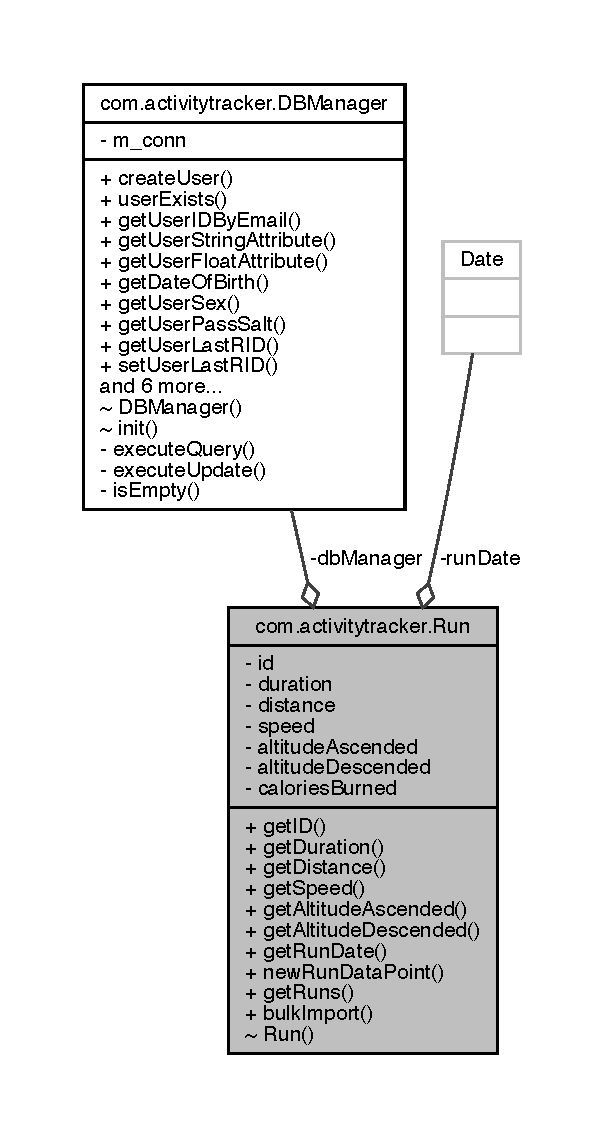
\includegraphics[width=290pt]{classcom_1_1activitytracker_1_1_run__coll__graph}
\end{center}
\end{figure}
\subsection*{Public Member Functions}
\begin{DoxyCompactItemize}
\item 
int \mbox{\hyperlink{classcom_1_1activitytracker_1_1_run_a61916c14ab5a2bf6b080200f7d0c5566}{get\+ID}} ()
\item 
float \mbox{\hyperlink{classcom_1_1activitytracker_1_1_run_af0d3f62a282a94fe74a1bdfa0c3dc277}{get\+Duration}} ()
\item 
float \mbox{\hyperlink{classcom_1_1activitytracker_1_1_run_a2d3b805547023d02f99634e09c6fa086}{get\+Distance}} ()
\item 
float \mbox{\hyperlink{classcom_1_1activitytracker_1_1_run_a913fd24db87de94db1c6decaad51e5f1}{get\+Speed}} ()
\item 
float \mbox{\hyperlink{classcom_1_1activitytracker_1_1_run_a9365647310eee181b15a85eaf6b95e93}{get\+Altitude\+Ascended}} ()
\item 
float \mbox{\hyperlink{classcom_1_1activitytracker_1_1_run_a75d18e68f984a4f5481e25f2c70f0492}{get\+Altitude\+Descended}} ()
\item 
Date \mbox{\hyperlink{classcom_1_1activitytracker_1_1_run_a3673ace303ad8026cdc80a6d6e7e3533}{get\+Run\+Date}} ()
\end{DoxyCompactItemize}
\subsection*{Static Public Member Functions}
\begin{DoxyCompactItemize}
\item 
static void \mbox{\hyperlink{classcom_1_1activitytracker_1_1_run_a5dea6f1860431103d553ce770382afe0}{new\+Run\+Data\+Point}} (final \mbox{\hyperlink{classcom_1_1activitytracker_1_1_d_b_manager}{D\+B\+Manager}} \mbox{\hyperlink{classcom_1_1activitytracker_1_1_run_ab90e32eda9f4c671ae3575f971edca6b}{db\+Manager}}, final \mbox{\hyperlink{classcom_1_1activitytracker_1_1_user}{User}} user, final float \mbox{\hyperlink{classcom_1_1activitytracker_1_1_run_a5e38d293d29d4b65c9290ff4bee82e03}{duration}}, final Date date, final float \mbox{\hyperlink{classcom_1_1activitytracker_1_1_run_a7b4ca8c4ecea4da1653f03b8c8fc16a8}{distance}}, final float altitude)
\item 
static Vector$<$ \mbox{\hyperlink{classcom_1_1activitytracker_1_1_run}{Run}} $>$ \mbox{\hyperlink{classcom_1_1activitytracker_1_1_run_a1aa1fb01eabff586e16d88f19f7df743}{get\+Runs}} (final \mbox{\hyperlink{classcom_1_1activitytracker_1_1_d_b_manager}{D\+B\+Manager}} \mbox{\hyperlink{classcom_1_1activitytracker_1_1_run_ab90e32eda9f4c671ae3575f971edca6b}{db\+Manager}}, final \mbox{\hyperlink{classcom_1_1activitytracker_1_1_user}{User}} user, final Date start\+Date, final Date end\+Date)
\item 
static void \mbox{\hyperlink{classcom_1_1activitytracker_1_1_run_a8e2b13e0096b87614d5333ec15213300}{bulk\+Import}} (final \mbox{\hyperlink{classcom_1_1activitytracker_1_1_d_b_manager}{D\+B\+Manager}} \mbox{\hyperlink{classcom_1_1activitytracker_1_1_run_ab90e32eda9f4c671ae3575f971edca6b}{db\+Manager}}, final \mbox{\hyperlink{classcom_1_1activitytracker_1_1_user}{User}} user, final String file\+Path)  throws File\+Not\+Found\+Exception, I\+O\+Exception 
\end{DoxyCompactItemize}
\subsection*{Package Functions}
\begin{DoxyCompactItemize}
\item 
\mbox{\hyperlink{classcom_1_1activitytracker_1_1_run_a5568c1c514835056d2abc22cfba222c5}{Run}} (final \mbox{\hyperlink{classcom_1_1activitytracker_1_1_d_b_manager}{D\+B\+Manager}} \mbox{\hyperlink{classcom_1_1activitytracker_1_1_run_ab90e32eda9f4c671ae3575f971edca6b}{db\+Manager}}, final int r\+ID)
\end{DoxyCompactItemize}
\subsection*{Private Attributes}
\begin{DoxyCompactItemize}
\item 
int \mbox{\hyperlink{classcom_1_1activitytracker_1_1_run_aa76717aee690b5bfe919d6e87dea1d84}{id}}
\item 
\mbox{\hyperlink{classcom_1_1activitytracker_1_1_d_b_manager}{D\+B\+Manager}} \mbox{\hyperlink{classcom_1_1activitytracker_1_1_run_ab90e32eda9f4c671ae3575f971edca6b}{db\+Manager}}
\item 
float \mbox{\hyperlink{classcom_1_1activitytracker_1_1_run_a5e38d293d29d4b65c9290ff4bee82e03}{duration}}
\item 
float \mbox{\hyperlink{classcom_1_1activitytracker_1_1_run_a7b4ca8c4ecea4da1653f03b8c8fc16a8}{distance}}
\item 
float \mbox{\hyperlink{classcom_1_1activitytracker_1_1_run_ada0c6e189d55997133cde5bbe9913984}{speed}}
\item 
float \mbox{\hyperlink{classcom_1_1activitytracker_1_1_run_ad28bf8d709b4cfcdb93a51033a90728c}{altitude\+Ascended}}
\item 
float \mbox{\hyperlink{classcom_1_1activitytracker_1_1_run_a4997349f78c9147a30811306c2ab5223}{altitude\+Descended}}
\item 
Date \mbox{\hyperlink{classcom_1_1activitytracker_1_1_run_a2f519da043ea384f1ba0d156f4971367}{run\+Date}}
\item 
long \mbox{\hyperlink{classcom_1_1activitytracker_1_1_run_aa4c73467653a47d3b14ff6653bbab853}{calories\+Burned}}
\end{DoxyCompactItemize}


\subsection{Detailed Description}
Used to logically instantiate a run. 

Definition at line 19 of file Run.\+java.



\subsection{Constructor \& Destructor Documentation}
\mbox{\Hypertarget{classcom_1_1activitytracker_1_1_run_a5568c1c514835056d2abc22cfba222c5}\label{classcom_1_1activitytracker_1_1_run_a5568c1c514835056d2abc22cfba222c5}} 
\index{com\+::activitytracker\+::\+Run@{com\+::activitytracker\+::\+Run}!Run@{Run}}
\index{Run@{Run}!com\+::activitytracker\+::\+Run@{com\+::activitytracker\+::\+Run}}
\subsubsection{\texorpdfstring{Run()}{Run()}}
{\footnotesize\ttfamily com.\+activitytracker.\+Run.\+Run (\begin{DoxyParamCaption}\item[{final \mbox{\hyperlink{classcom_1_1activitytracker_1_1_d_b_manager}{D\+B\+Manager}}}]{db\+Manager,  }\item[{final int}]{r\+ID }\end{DoxyParamCaption})\hspace{0.3cm}{\ttfamily [package]}}

The \mbox{\hyperlink{classcom_1_1activitytracker_1_1_run_a5568c1c514835056d2abc22cfba222c5}{Run()}} constructor is used to retrieve workout information from the database and instantiate each row of the Runs table in a logical format.


\begin{DoxyParams}{Parameters}
{\em db\+Manager} & The connection to the database. \\
\hline
{\em r\+ID} & The run ID used to retrieve information from the database. \\
\hline
\end{DoxyParams}


Definition at line 66 of file Run.\+java.


\begin{DoxyCode}
66                                                    \{
67         this.\textcolor{keywordtype}{id} = rID;
68         this.\mbox{\hyperlink{classcom_1_1activitytracker_1_1_run_ab90e32eda9f4c671ae3575f971edca6b}{dbManager}} = \mbox{\hyperlink{classcom_1_1activitytracker_1_1_run_ab90e32eda9f4c671ae3575f971edca6b}{dbManager}};
69         this.\mbox{\hyperlink{classcom_1_1activitytracker_1_1_run_a2f519da043ea384f1ba0d156f4971367}{runDate}} = this.\mbox{\hyperlink{classcom_1_1activitytracker_1_1_run_ab90e32eda9f4c671ae3575f971edca6b}{dbManager}}.\mbox{\hyperlink{classcom_1_1activitytracker_1_1_d_b_manager_a1bef7a6f466db41b1a6da7a502d35bb9}{getRunDate}}(rID);
70         this.\mbox{\hyperlink{classcom_1_1activitytracker_1_1_run_a5e38d293d29d4b65c9290ff4bee82e03}{duration}} = this.\mbox{\hyperlink{classcom_1_1activitytracker_1_1_run_ab90e32eda9f4c671ae3575f971edca6b}{dbManager}}.\mbox{\hyperlink{classcom_1_1activitytracker_1_1_d_b_manager_a666452f1e5862f90c06b0beb9a9fcfdd}{getRunFloatAttribute}}(
      RunAttribute.DURATION, rID);
71         this.\mbox{\hyperlink{classcom_1_1activitytracker_1_1_run_a7b4ca8c4ecea4da1653f03b8c8fc16a8}{distance}} = this.\mbox{\hyperlink{classcom_1_1activitytracker_1_1_run_ab90e32eda9f4c671ae3575f971edca6b}{dbManager}}.\mbox{\hyperlink{classcom_1_1activitytracker_1_1_d_b_manager_a666452f1e5862f90c06b0beb9a9fcfdd}{getRunFloatAttribute}}(
      RunAttribute.DISTANCE, rID);
72         this.\mbox{\hyperlink{classcom_1_1activitytracker_1_1_run_ada0c6e189d55997133cde5bbe9913984}{speed}} = this.\mbox{\hyperlink{classcom_1_1activitytracker_1_1_run_a7b4ca8c4ecea4da1653f03b8c8fc16a8}{distance}} / this.\mbox{\hyperlink{classcom_1_1activitytracker_1_1_run_a5e38d293d29d4b65c9290ff4bee82e03}{duration}};
73         this.\mbox{\hyperlink{classcom_1_1activitytracker_1_1_run_ad28bf8d709b4cfcdb93a51033a90728c}{altitudeAscended}} = this.\mbox{\hyperlink{classcom_1_1activitytracker_1_1_run_ab90e32eda9f4c671ae3575f971edca6b}{dbManager}}.
      \mbox{\hyperlink{classcom_1_1activitytracker_1_1_d_b_manager_a666452f1e5862f90c06b0beb9a9fcfdd}{getRunFloatAttribute}}(RunAttribute.ALTITUDE\_ASCENDED, rID);
74         this.\mbox{\hyperlink{classcom_1_1activitytracker_1_1_run_a4997349f78c9147a30811306c2ab5223}{altitudeDescended}} = this.\mbox{\hyperlink{classcom_1_1activitytracker_1_1_run_ab90e32eda9f4c671ae3575f971edca6b}{dbManager}}.
      \mbox{\hyperlink{classcom_1_1activitytracker_1_1_d_b_manager_a666452f1e5862f90c06b0beb9a9fcfdd}{getRunFloatAttribute}}(RunAttribute.ALTITUDE\_DESCENDED, rID);
75         this.\mbox{\hyperlink{classcom_1_1activitytracker_1_1_run_aa4c73467653a47d3b14ff6653bbab853}{caloriesBurned}} = 0;
76     \}
\end{DoxyCode}


\subsection{Member Function Documentation}
\mbox{\Hypertarget{classcom_1_1activitytracker_1_1_run_a8e2b13e0096b87614d5333ec15213300}\label{classcom_1_1activitytracker_1_1_run_a8e2b13e0096b87614d5333ec15213300}} 
\index{com\+::activitytracker\+::\+Run@{com\+::activitytracker\+::\+Run}!bulk\+Import@{bulk\+Import}}
\index{bulk\+Import@{bulk\+Import}!com\+::activitytracker\+::\+Run@{com\+::activitytracker\+::\+Run}}
\subsubsection{\texorpdfstring{bulk\+Import()}{bulkImport()}}
{\footnotesize\ttfamily static void com.\+activitytracker.\+Run.\+bulk\+Import (\begin{DoxyParamCaption}\item[{final \mbox{\hyperlink{classcom_1_1activitytracker_1_1_d_b_manager}{D\+B\+Manager}}}]{db\+Manager,  }\item[{final \mbox{\hyperlink{classcom_1_1activitytracker_1_1_user}{User}}}]{user,  }\item[{final String}]{file\+Path }\end{DoxyParamCaption}) throws File\+Not\+Found\+Exception, I\+O\+Exception\hspace{0.3cm}{\ttfamily [static]}}

Opens and iterates through a file. The \mbox{\hyperlink{classcom_1_1activitytracker_1_1_run_a5dea6f1860431103d553ce770382afe0}{Run\+::new\+Run\+Data\+Point()}} method is called for each line.


\begin{DoxyParams}{Parameters}
{\em db\+Manager} & Database connection with with the method interacts. \\
\hline
{\em user} & A \mbox{\hyperlink{classcom_1_1activitytracker_1_1_user}{User}} object corresponding to the use whose run(s) is/are being retrieved from the database. \\
\hline
{\em file\+Path} & The file to be iterated through\\
\hline
\end{DoxyParams}

\begin{DoxyExceptions}{Exceptions}
{\em File\+Not\+Found\+Exception} & Thrown if the file path given does not exist. \\
\hline
{\em I\+O\+Exception} & Thrown if there is an error reading or opening the file. \\
\hline
\end{DoxyExceptions}


Definition at line 193 of file Run.\+java.


\begin{DoxyCode}
194                                                       \{
195         BufferedReader br = \textcolor{keyword}{new} BufferedReader(\textcolor{keyword}{new} FileReader(filePath));
196         String line = null;
197         Date date = null;
198         \textcolor{keywordflow}{while} ((line = br.readLine()) != null)  
199         \{
200             String[] attributes = line.split(\textcolor{stringliteral}{","});
201             String buffTime = attributes[0];
202             String buffDistance = attributes[1];
203             String buffAltitude = attributes[2];
204             String buffDate = attributes[3];
205             DateFormat sourceFormat = \textcolor{keyword}{new} SimpleDateFormat(\textcolor{stringliteral}{"dd-MM-yyyy"});
206             \textcolor{keywordflow}{try} \{
207                 date = sourceFormat.parse(buffDate);
208             \}
209             \textcolor{keywordflow}{catch} (\textcolor{keyword}{final} ParseException e) \{
210                 System.err.println(e.getMessage());
211             \}
212 
213             \textcolor{comment}{// Convert strings to floats}
214             \textcolor{keywordtype}{float} fDur = Float.parseFloat(buffTime);
215             \textcolor{keywordtype}{float} fDist = Float.parseFloat(buffDistance);
216             \textcolor{keywordtype}{float} fAlt = Float.parseFloat(buffAltitude);
217 
218             \mbox{\hyperlink{classcom_1_1activitytracker_1_1_run_a5dea6f1860431103d553ce770382afe0}{newRunDataPoint}}(\mbox{\hyperlink{classcom_1_1activitytracker_1_1_run_ab90e32eda9f4c671ae3575f971edca6b}{dbManager}}, user, fDur, date, fDist, fAlt);
219         \} 
220     \}
\end{DoxyCode}
\mbox{\Hypertarget{classcom_1_1activitytracker_1_1_run_a9365647310eee181b15a85eaf6b95e93}\label{classcom_1_1activitytracker_1_1_run_a9365647310eee181b15a85eaf6b95e93}} 
\index{com\+::activitytracker\+::\+Run@{com\+::activitytracker\+::\+Run}!get\+Altitude\+Ascended@{get\+Altitude\+Ascended}}
\index{get\+Altitude\+Ascended@{get\+Altitude\+Ascended}!com\+::activitytracker\+::\+Run@{com\+::activitytracker\+::\+Run}}
\subsubsection{\texorpdfstring{get\+Altitude\+Ascended()}{getAltitudeAscended()}}
{\footnotesize\ttfamily float com.\+activitytracker.\+Run.\+get\+Altitude\+Ascended (\begin{DoxyParamCaption}{ }\end{DoxyParamCaption})}

Retrieves a \mbox{\hyperlink{classcom_1_1activitytracker_1_1_run}{Run}} object\textquotesingle{}s altitude ascended (in metres).

\begin{DoxyReturn}{Returns}
The \mbox{\hyperlink{classcom_1_1activitytracker_1_1_run}{Run}}\textquotesingle{}s altitude ascended as defined in the database. 
\end{DoxyReturn}


Definition at line 263 of file Run.\+java.


\begin{DoxyCode}
263                                        \{
264         BigDecimal a = \textcolor{keyword}{new} BigDecimal(\mbox{\hyperlink{classcom_1_1activitytracker_1_1_run_ad28bf8d709b4cfcdb93a51033a90728c}{altitudeAscended}});
265         \textcolor{keywordflow}{return} a.setScale(3, RoundingMode.UP).floatValue();
266     \}
\end{DoxyCode}
\mbox{\Hypertarget{classcom_1_1activitytracker_1_1_run_a75d18e68f984a4f5481e25f2c70f0492}\label{classcom_1_1activitytracker_1_1_run_a75d18e68f984a4f5481e25f2c70f0492}} 
\index{com\+::activitytracker\+::\+Run@{com\+::activitytracker\+::\+Run}!get\+Altitude\+Descended@{get\+Altitude\+Descended}}
\index{get\+Altitude\+Descended@{get\+Altitude\+Descended}!com\+::activitytracker\+::\+Run@{com\+::activitytracker\+::\+Run}}
\subsubsection{\texorpdfstring{get\+Altitude\+Descended()}{getAltitudeDescended()}}
{\footnotesize\ttfamily float com.\+activitytracker.\+Run.\+get\+Altitude\+Descended (\begin{DoxyParamCaption}{ }\end{DoxyParamCaption})}

Retrieves a \mbox{\hyperlink{classcom_1_1activitytracker_1_1_run}{Run}} object\textquotesingle{}s altitude descended (in metres).

\begin{DoxyReturn}{Returns}
The \mbox{\hyperlink{classcom_1_1activitytracker_1_1_run}{Run}}\textquotesingle{}s altitude descended as defined in the database. 
\end{DoxyReturn}


Definition at line 273 of file Run.\+java.


\begin{DoxyCode}
273                                         \{
274         BigDecimal a = \textcolor{keyword}{new} BigDecimal(\mbox{\hyperlink{classcom_1_1activitytracker_1_1_run_a4997349f78c9147a30811306c2ab5223}{altitudeDescended}});
275         \textcolor{keywordflow}{return} a.setScale(3, RoundingMode.UP).floatValue();
276     \}
\end{DoxyCode}
\mbox{\Hypertarget{classcom_1_1activitytracker_1_1_run_a2d3b805547023d02f99634e09c6fa086}\label{classcom_1_1activitytracker_1_1_run_a2d3b805547023d02f99634e09c6fa086}} 
\index{com\+::activitytracker\+::\+Run@{com\+::activitytracker\+::\+Run}!get\+Distance@{get\+Distance}}
\index{get\+Distance@{get\+Distance}!com\+::activitytracker\+::\+Run@{com\+::activitytracker\+::\+Run}}
\subsubsection{\texorpdfstring{get\+Distance()}{getDistance()}}
{\footnotesize\ttfamily float com.\+activitytracker.\+Run.\+get\+Distance (\begin{DoxyParamCaption}{ }\end{DoxyParamCaption})}

Retrieves a \mbox{\hyperlink{classcom_1_1activitytracker_1_1_run}{Run}} object\textquotesingle{}s distance (in metres).

\begin{DoxyReturn}{Returns}
The \mbox{\hyperlink{classcom_1_1activitytracker_1_1_run}{Run}}\textquotesingle{}s distance as defined in the database. 
\end{DoxyReturn}


Definition at line 245 of file Run.\+java.


\begin{DoxyCode}
245                                \{
246         \textcolor{keywordflow}{return} \mbox{\hyperlink{classcom_1_1activitytracker_1_1_run_a7b4ca8c4ecea4da1653f03b8c8fc16a8}{distance}};
247     \}
\end{DoxyCode}
\mbox{\Hypertarget{classcom_1_1activitytracker_1_1_run_af0d3f62a282a94fe74a1bdfa0c3dc277}\label{classcom_1_1activitytracker_1_1_run_af0d3f62a282a94fe74a1bdfa0c3dc277}} 
\index{com\+::activitytracker\+::\+Run@{com\+::activitytracker\+::\+Run}!get\+Duration@{get\+Duration}}
\index{get\+Duration@{get\+Duration}!com\+::activitytracker\+::\+Run@{com\+::activitytracker\+::\+Run}}
\subsubsection{\texorpdfstring{get\+Duration()}{getDuration()}}
{\footnotesize\ttfamily float com.\+activitytracker.\+Run.\+get\+Duration (\begin{DoxyParamCaption}{ }\end{DoxyParamCaption})}

Retrieves a \mbox{\hyperlink{classcom_1_1activitytracker_1_1_run}{Run}} object\textquotesingle{}s duration (in seconds).

\begin{DoxyReturn}{Returns}
The \mbox{\hyperlink{classcom_1_1activitytracker_1_1_run}{Run}}\textquotesingle{}s duration as defined in the database. 
\end{DoxyReturn}


Definition at line 236 of file Run.\+java.


\begin{DoxyCode}
236                                \{
237         \textcolor{keywordflow}{return} \mbox{\hyperlink{classcom_1_1activitytracker_1_1_run_a5e38d293d29d4b65c9290ff4bee82e03}{duration}};
238     \}
\end{DoxyCode}
\mbox{\Hypertarget{classcom_1_1activitytracker_1_1_run_a61916c14ab5a2bf6b080200f7d0c5566}\label{classcom_1_1activitytracker_1_1_run_a61916c14ab5a2bf6b080200f7d0c5566}} 
\index{com\+::activitytracker\+::\+Run@{com\+::activitytracker\+::\+Run}!get\+ID@{get\+ID}}
\index{get\+ID@{get\+ID}!com\+::activitytracker\+::\+Run@{com\+::activitytracker\+::\+Run}}
\subsubsection{\texorpdfstring{get\+I\+D()}{getID()}}
{\footnotesize\ttfamily int com.\+activitytracker.\+Run.\+get\+ID (\begin{DoxyParamCaption}{ }\end{DoxyParamCaption})}

Retrieves a \mbox{\hyperlink{classcom_1_1activitytracker_1_1_run}{Run}} object\textquotesingle{}s ID.

\begin{DoxyReturn}{Returns}
The \mbox{\hyperlink{classcom_1_1activitytracker_1_1_run}{Run}}\textquotesingle{}s ID as defined in the database. 
\end{DoxyReturn}


Definition at line 227 of file Run.\+java.


\begin{DoxyCode}
227                        \{
228         \textcolor{keywordflow}{return} this.\mbox{\hyperlink{classcom_1_1activitytracker_1_1_run_aa76717aee690b5bfe919d6e87dea1d84}{id}};
229     \}
\end{DoxyCode}
\mbox{\Hypertarget{classcom_1_1activitytracker_1_1_run_a3673ace303ad8026cdc80a6d6e7e3533}\label{classcom_1_1activitytracker_1_1_run_a3673ace303ad8026cdc80a6d6e7e3533}} 
\index{com\+::activitytracker\+::\+Run@{com\+::activitytracker\+::\+Run}!get\+Run\+Date@{get\+Run\+Date}}
\index{get\+Run\+Date@{get\+Run\+Date}!com\+::activitytracker\+::\+Run@{com\+::activitytracker\+::\+Run}}
\subsubsection{\texorpdfstring{get\+Run\+Date()}{getRunDate()}}
{\footnotesize\ttfamily Date com.\+activitytracker.\+Run.\+get\+Run\+Date (\begin{DoxyParamCaption}{ }\end{DoxyParamCaption})}

Retrieves a \mbox{\hyperlink{classcom_1_1activitytracker_1_1_run}{Run}} object\textquotesingle{}s date.

\begin{DoxyReturn}{Returns}
The \mbox{\hyperlink{classcom_1_1activitytracker_1_1_run}{Run}}\textquotesingle{}s date. 
\end{DoxyReturn}


Definition at line 283 of file Run.\+java.


\begin{DoxyCode}
283                              \{
284         \textcolor{keywordflow}{return} \mbox{\hyperlink{classcom_1_1activitytracker_1_1_run_a2f519da043ea384f1ba0d156f4971367}{runDate}};
285     \}
\end{DoxyCode}
\mbox{\Hypertarget{classcom_1_1activitytracker_1_1_run_a1aa1fb01eabff586e16d88f19f7df743}\label{classcom_1_1activitytracker_1_1_run_a1aa1fb01eabff586e16d88f19f7df743}} 
\index{com\+::activitytracker\+::\+Run@{com\+::activitytracker\+::\+Run}!get\+Runs@{get\+Runs}}
\index{get\+Runs@{get\+Runs}!com\+::activitytracker\+::\+Run@{com\+::activitytracker\+::\+Run}}
\subsubsection{\texorpdfstring{get\+Runs()}{getRuns()}}
{\footnotesize\ttfamily static Vector$<$\mbox{\hyperlink{classcom_1_1activitytracker_1_1_run}{Run}}$>$ com.\+activitytracker.\+Run.\+get\+Runs (\begin{DoxyParamCaption}\item[{final \mbox{\hyperlink{classcom_1_1activitytracker_1_1_d_b_manager}{D\+B\+Manager}}}]{db\+Manager,  }\item[{final \mbox{\hyperlink{classcom_1_1activitytracker_1_1_user}{User}}}]{user,  }\item[{final Date}]{start\+Date,  }\item[{final Date}]{end\+Date }\end{DoxyParamCaption})\hspace{0.3cm}{\ttfamily [static]}}

Retrieves a set of runs from the database. Returns the result as a vector of \mbox{\hyperlink{classcom_1_1activitytracker_1_1_run}{Run}} objects.


\begin{DoxyParams}{Parameters}
{\em db\+Manager} & Database connection with with the method interacts. \\
\hline
{\em user} & A \mbox{\hyperlink{classcom_1_1activitytracker_1_1_user}{User}} object corresponding to the use whose run(s) is/are being retrieved from the database. \\
\hline
{\em start\+Date} & The beginning of the interval for which we are retrieving workouts. \\
\hline
{\em end\+Date} & The end of the interval for which we are retrieving workouts.\\
\hline
\end{DoxyParams}
\begin{DoxyReturn}{Returns}
A vector containing instances of \mbox{\hyperlink{classcom_1_1activitytracker_1_1_run}{Run}} corresponding to all entered workouts between the start and end dates specified. 
\end{DoxyReturn}


Definition at line 162 of file Run.\+java.


\begin{DoxyCode}
163                                                                                 \{
164         Vector<Run> runs = \textcolor{keyword}{new} Vector<>();
165         \textcolor{keywordtype}{int} rID;
166         Vector<Integer> rIDs = \mbox{\hyperlink{classcom_1_1activitytracker_1_1_run_ab90e32eda9f4c671ae3575f971edca6b}{dbManager}}.\mbox{\hyperlink{classcom_1_1activitytracker_1_1_d_b_manager_a48d9e51c1b73064b8f773cdde5113928}{getRuns}}(user.getID(), startDate, endDate);
167 
168         \textcolor{keywordflow}{if} (rIDs != null) \{
169             Iterator<Integer> runIDIter = rIDs.iterator();
170             \textcolor{keywordflow}{while} (runIDIter.hasNext()) \{
171                 rID = runIDIter.next();
172                 runs.add(\textcolor{keyword}{new} \mbox{\hyperlink{classcom_1_1activitytracker_1_1_run_a5568c1c514835056d2abc22cfba222c5}{Run}}(\mbox{\hyperlink{classcom_1_1activitytracker_1_1_run_ab90e32eda9f4c671ae3575f971edca6b}{dbManager}}, rID));
173             \}
174             \textcolor{keywordflow}{return} runs;
175         \}
176         \textcolor{keywordflow}{else} \{
177             System.err.println(\textcolor{stringliteral}{"DBManager.getRuns() returned null."});
178             \textcolor{keywordflow}{return} null;
179         \}
180     \}
\end{DoxyCode}
\mbox{\Hypertarget{classcom_1_1activitytracker_1_1_run_a913fd24db87de94db1c6decaad51e5f1}\label{classcom_1_1activitytracker_1_1_run_a913fd24db87de94db1c6decaad51e5f1}} 
\index{com\+::activitytracker\+::\+Run@{com\+::activitytracker\+::\+Run}!get\+Speed@{get\+Speed}}
\index{get\+Speed@{get\+Speed}!com\+::activitytracker\+::\+Run@{com\+::activitytracker\+::\+Run}}
\subsubsection{\texorpdfstring{get\+Speed()}{getSpeed()}}
{\footnotesize\ttfamily float com.\+activitytracker.\+Run.\+get\+Speed (\begin{DoxyParamCaption}{ }\end{DoxyParamCaption})}

Retrieves a \mbox{\hyperlink{classcom_1_1activitytracker_1_1_run}{Run}} object\textquotesingle{}s average speed (in metres per second).

\begin{DoxyReturn}{Returns}
The \mbox{\hyperlink{classcom_1_1activitytracker_1_1_run}{Run}}\textquotesingle{}s average speed as computed in the \mbox{\hyperlink{classcom_1_1activitytracker_1_1_run_a5568c1c514835056d2abc22cfba222c5}{Run()}} constructor. 
\end{DoxyReturn}


Definition at line 254 of file Run.\+java.


\begin{DoxyCode}
254                             \{
255         \textcolor{keywordflow}{return} \mbox{\hyperlink{classcom_1_1activitytracker_1_1_run_ada0c6e189d55997133cde5bbe9913984}{speed}};
256     \}
\end{DoxyCode}
\mbox{\Hypertarget{classcom_1_1activitytracker_1_1_run_a5dea6f1860431103d553ce770382afe0}\label{classcom_1_1activitytracker_1_1_run_a5dea6f1860431103d553ce770382afe0}} 
\index{com\+::activitytracker\+::\+Run@{com\+::activitytracker\+::\+Run}!new\+Run\+Data\+Point@{new\+Run\+Data\+Point}}
\index{new\+Run\+Data\+Point@{new\+Run\+Data\+Point}!com\+::activitytracker\+::\+Run@{com\+::activitytracker\+::\+Run}}
\subsubsection{\texorpdfstring{new\+Run\+Data\+Point()}{newRunDataPoint()}}
{\footnotesize\ttfamily static void com.\+activitytracker.\+Run.\+new\+Run\+Data\+Point (\begin{DoxyParamCaption}\item[{final \mbox{\hyperlink{classcom_1_1activitytracker_1_1_d_b_manager}{D\+B\+Manager}}}]{db\+Manager,  }\item[{final \mbox{\hyperlink{classcom_1_1activitytracker_1_1_user}{User}}}]{user,  }\item[{final float}]{duration,  }\item[{final Date}]{date,  }\item[{final float}]{distance,  }\item[{final float}]{altitude }\end{DoxyParamCaption})\hspace{0.3cm}{\ttfamily [static]}}

Adds a new workout to the database or updates an existing workout with new information that the user imported from the log file.

If ({\itshape duration}, {\itshape distance}, {\itshape altitude}) passed to this method is (0, 0, 0) then the intended assumption is that this is the beginning of a new workout. As such, this input will cause a new row to be added to the Runs table in the database and the user\textquotesingle{}s last run ID attribute will be updated accordingly. If the input is non-\/(0, 0, 0), then three things take place\+:
\begin{DoxyEnumerate}
\item The {\itshape duration} in the database is overwritten by the {\itshape duration} provided as input;
\item The {\itshape distance} in the database is overwritten by the {\itshape distance} provided as input; and
\item Existing values for {\itshape altitude\+\_\+ascended} and {\itshape altitude\+\_\+descended} are retrieved from the database, their difference is compared to the current relative altitude, and depending whether this difference is positive or negative, the appropriate field in the database is updated to reflect the change.
\end{DoxyEnumerate}


\begin{DoxyParams}{Parameters}
{\em db\+Manager} & Database connection with with the method interacts. \\
\hline
{\em user} & A \mbox{\hyperlink{classcom_1_1activitytracker_1_1_user}{User}} object corresponding to the use whose run is being added to the database. \\
\hline
{\em duration} & The length of time in seconds that the user\textquotesingle{}s run lasted. \\
\hline
{\em date} & The date the run occurred. \\
\hline
{\em distance} & The cumulative distance (in metres) that the user ran as of the current time passed to the method. \\
\hline
{\em altitude} & The relative current altitude (in metres) of the user at the time point being entered. Used to compute cumulative altitude ascended and descended throughout the run. \\
\hline
\end{DoxyParams}


Definition at line 102 of file Run.\+java.


\begin{DoxyCode}
103                                                                                                \{
104         \textcolor{keywordtype}{int} userID = user.getID();
105         \textcolor{keywordtype}{int} rID;
106         \textcolor{keywordtype}{float} altitude\_ascended;
107         \textcolor{keywordtype}{float} altitude\_descended;
108 
109         \textcolor{keywordflow}{if} (\mbox{\hyperlink{classcom_1_1activitytracker_1_1_run_a5e38d293d29d4b65c9290ff4bee82e03}{duration}} == 0f && \mbox{\hyperlink{classcom_1_1activitytracker_1_1_run_a7b4ca8c4ecea4da1653f03b8c8fc16a8}{distance}} == 0f && altitude == 0f) \{
110             altitude\_ascended = 0f;
111             altitude\_descended = 0f;
112             rID = \mbox{\hyperlink{classcom_1_1activitytracker_1_1_run_ab90e32eda9f4c671ae3575f971edca6b}{dbManager}}.\mbox{\hyperlink{classcom_1_1activitytracker_1_1_d_b_manager_ae0504a939b6f165aa5c3cca9eb8df049}{newRun}}(
113                     userID,
114                     date,
115                     \mbox{\hyperlink{classcom_1_1activitytracker_1_1_run_a5e38d293d29d4b65c9290ff4bee82e03}{duration}},
116                     \mbox{\hyperlink{classcom_1_1activitytracker_1_1_run_a7b4ca8c4ecea4da1653f03b8c8fc16a8}{distance}},
117                     altitude\_ascended,
118                     altitude\_descended
119             );
120             user.setLastRID(rID);
121             System.err.println(\textcolor{stringliteral}{"Run "} + Integer.toString(rID) + \textcolor{stringliteral}{" added to database."});
122         \} \textcolor{keywordflow}{else} \{
123             rID = user.getLastRID();
124             \textcolor{keywordflow}{if} (\mbox{\hyperlink{classcom_1_1activitytracker_1_1_run_ab90e32eda9f4c671ae3575f971edca6b}{dbManager}}.\mbox{\hyperlink{classcom_1_1activitytracker_1_1_d_b_manager_a723ac1c573bacdd0b62894357bd65a9b}{runExists}}(rID)) \{
125                 altitude\_ascended = \mbox{\hyperlink{classcom_1_1activitytracker_1_1_run_ab90e32eda9f4c671ae3575f971edca6b}{dbManager}}.\mbox{\hyperlink{classcom_1_1activitytracker_1_1_d_b_manager_a666452f1e5862f90c06b0beb9a9fcfdd}{getRunFloatAttribute}}(
      RunAttribute.ALTITUDE\_ASCENDED, rID);
126                 altitude\_descended = \mbox{\hyperlink{classcom_1_1activitytracker_1_1_run_ab90e32eda9f4c671ae3575f971edca6b}{dbManager}}.\mbox{\hyperlink{classcom_1_1activitytracker_1_1_d_b_manager_a666452f1e5862f90c06b0beb9a9fcfdd}{getRunFloatAttribute}}(
      RunAttribute.ALTITUDE\_DESCENDED, rID);
127 
128                 System.err.println(\textcolor{stringliteral}{"Altitude: "} + Float.toString(altitude) + \textcolor{stringliteral}{", +: "} + Float.toString(
      altitude\_ascended) + \textcolor{stringliteral}{", -: "} + Float.toString(altitude\_descended));
129                 \textcolor{keywordflow}{if} (altitude < altitude\_ascended-altitude\_descended) \{
130                     altitude\_descended += altitude\_ascended - altitude\_descended - altitude;
131                     System.err.println(\textcolor{stringliteral}{"Went down "} + Float.toString(altitude\_ascended - altitude\_descended
       - altitude));
132                 \}
133                 \textcolor{keywordflow}{else} \{
134                     altitude\_ascended += altitude - (altitude\_ascended - altitude\_descended);
135                     System.err.println(\textcolor{stringliteral}{"Went up "} + Float.toString(altitude - altitude\_ascended - 
      altitude\_descended));
136                 \}
137 
138                 \mbox{\hyperlink{classcom_1_1activitytracker_1_1_run_ab90e32eda9f4c671ae3575f971edca6b}{dbManager}}.\mbox{\hyperlink{classcom_1_1activitytracker_1_1_d_b_manager_aa088e156858d8d661e2f43c1054c51c8}{setRun}}(rID, \mbox{\hyperlink{classcom_1_1activitytracker_1_1_run_a5e38d293d29d4b65c9290ff4bee82e03}{duration}}, \mbox{\hyperlink{classcom_1_1activitytracker_1_1_run_a7b4ca8c4ecea4da1653f03b8c8fc16a8}{distance}}, altitude\_ascended,
       altitude\_descended);
139                 System.err.println(\textcolor{stringliteral}{"Run "} + Integer.toString(rID) + \textcolor{stringliteral}{" exists in the database; updating..."})
      ;
140             \} \textcolor{keywordflow}{else} \{
141                 System.err.println(\textcolor{stringliteral}{"Run table and User table are inconsistent. No changes made."});
142             \}
143         \}
144 
145         altitude\_ascended = \mbox{\hyperlink{classcom_1_1activitytracker_1_1_run_ab90e32eda9f4c671ae3575f971edca6b}{dbManager}}.\mbox{\hyperlink{classcom_1_1activitytracker_1_1_d_b_manager_a666452f1e5862f90c06b0beb9a9fcfdd}{getRunFloatAttribute}}(RunAttribute.
      ALTITUDE\_ASCENDED, rID);
146         altitude\_descended = \mbox{\hyperlink{classcom_1_1activitytracker_1_1_run_ab90e32eda9f4c671ae3575f971edca6b}{dbManager}}.\mbox{\hyperlink{classcom_1_1activitytracker_1_1_d_b_manager_a666452f1e5862f90c06b0beb9a9fcfdd}{getRunFloatAttribute}}(RunAttribute.
      ALTITUDE\_DESCENDED, rID);
147 
148         System.err.println(\textcolor{stringliteral}{"+: "} + Float.toString(altitude\_ascended) + \textcolor{stringliteral}{", -: "} + Float.toString(
      altitude\_descended));
149     \}
\end{DoxyCode}


\subsection{Member Data Documentation}
\mbox{\Hypertarget{classcom_1_1activitytracker_1_1_run_ad28bf8d709b4cfcdb93a51033a90728c}\label{classcom_1_1activitytracker_1_1_run_ad28bf8d709b4cfcdb93a51033a90728c}} 
\index{com\+::activitytracker\+::\+Run@{com\+::activitytracker\+::\+Run}!altitude\+Ascended@{altitude\+Ascended}}
\index{altitude\+Ascended@{altitude\+Ascended}!com\+::activitytracker\+::\+Run@{com\+::activitytracker\+::\+Run}}
\subsubsection{\texorpdfstring{altitude\+Ascended}{altitudeAscended}}
{\footnotesize\ttfamily float com.\+activitytracker.\+Run.\+altitude\+Ascended\hspace{0.3cm}{\ttfamily [private]}}

The altitude (in metres) that the user climed throughout the run. 

Definition at line 43 of file Run.\+java.

\mbox{\Hypertarget{classcom_1_1activitytracker_1_1_run_a4997349f78c9147a30811306c2ab5223}\label{classcom_1_1activitytracker_1_1_run_a4997349f78c9147a30811306c2ab5223}} 
\index{com\+::activitytracker\+::\+Run@{com\+::activitytracker\+::\+Run}!altitude\+Descended@{altitude\+Descended}}
\index{altitude\+Descended@{altitude\+Descended}!com\+::activitytracker\+::\+Run@{com\+::activitytracker\+::\+Run}}
\subsubsection{\texorpdfstring{altitude\+Descended}{altitudeDescended}}
{\footnotesize\ttfamily float com.\+activitytracker.\+Run.\+altitude\+Descended\hspace{0.3cm}{\ttfamily [private]}}

The altitude (in metres) that the user descended throughout their run. 

Definition at line 47 of file Run.\+java.

\mbox{\Hypertarget{classcom_1_1activitytracker_1_1_run_aa4c73467653a47d3b14ff6653bbab853}\label{classcom_1_1activitytracker_1_1_run_aa4c73467653a47d3b14ff6653bbab853}} 
\index{com\+::activitytracker\+::\+Run@{com\+::activitytracker\+::\+Run}!calories\+Burned@{calories\+Burned}}
\index{calories\+Burned@{calories\+Burned}!com\+::activitytracker\+::\+Run@{com\+::activitytracker\+::\+Run}}
\subsubsection{\texorpdfstring{calories\+Burned}{caloriesBurned}}
{\footnotesize\ttfamily long com.\+activitytracker.\+Run.\+calories\+Burned\hspace{0.3cm}{\ttfamily [private]}}

The number of calories that the user burned throughout their run.

Currently this is not being used; it is for future features. 

Definition at line 57 of file Run.\+java.

\mbox{\Hypertarget{classcom_1_1activitytracker_1_1_run_ab90e32eda9f4c671ae3575f971edca6b}\label{classcom_1_1activitytracker_1_1_run_ab90e32eda9f4c671ae3575f971edca6b}} 
\index{com\+::activitytracker\+::\+Run@{com\+::activitytracker\+::\+Run}!db\+Manager@{db\+Manager}}
\index{db\+Manager@{db\+Manager}!com\+::activitytracker\+::\+Run@{com\+::activitytracker\+::\+Run}}
\subsubsection{\texorpdfstring{db\+Manager}{dbManager}}
{\footnotesize\ttfamily \mbox{\hyperlink{classcom_1_1activitytracker_1_1_d_b_manager}{D\+B\+Manager}} com.\+activitytracker.\+Run.\+db\+Manager\hspace{0.3cm}{\ttfamily [private]}}

The run\textquotesingle{}s connection to the database. This is used to add data points and retrieve workout metadata. 

Definition at line 27 of file Run.\+java.

\mbox{\Hypertarget{classcom_1_1activitytracker_1_1_run_a7b4ca8c4ecea4da1653f03b8c8fc16a8}\label{classcom_1_1activitytracker_1_1_run_a7b4ca8c4ecea4da1653f03b8c8fc16a8}} 
\index{com\+::activitytracker\+::\+Run@{com\+::activitytracker\+::\+Run}!distance@{distance}}
\index{distance@{distance}!com\+::activitytracker\+::\+Run@{com\+::activitytracker\+::\+Run}}
\subsubsection{\texorpdfstring{distance}{distance}}
{\footnotesize\ttfamily float com.\+activitytracker.\+Run.\+distance\hspace{0.3cm}{\ttfamily [private]}}

The distance (in metres) that the user ran. 

Definition at line 35 of file Run.\+java.

\mbox{\Hypertarget{classcom_1_1activitytracker_1_1_run_a5e38d293d29d4b65c9290ff4bee82e03}\label{classcom_1_1activitytracker_1_1_run_a5e38d293d29d4b65c9290ff4bee82e03}} 
\index{com\+::activitytracker\+::\+Run@{com\+::activitytracker\+::\+Run}!duration@{duration}}
\index{duration@{duration}!com\+::activitytracker\+::\+Run@{com\+::activitytracker\+::\+Run}}
\subsubsection{\texorpdfstring{duration}{duration}}
{\footnotesize\ttfamily float com.\+activitytracker.\+Run.\+duration\hspace{0.3cm}{\ttfamily [private]}}

The length of the run in seconds. 

Definition at line 31 of file Run.\+java.

\mbox{\Hypertarget{classcom_1_1activitytracker_1_1_run_aa76717aee690b5bfe919d6e87dea1d84}\label{classcom_1_1activitytracker_1_1_run_aa76717aee690b5bfe919d6e87dea1d84}} 
\index{com\+::activitytracker\+::\+Run@{com\+::activitytracker\+::\+Run}!id@{id}}
\index{id@{id}!com\+::activitytracker\+::\+Run@{com\+::activitytracker\+::\+Run}}
\subsubsection{\texorpdfstring{id}{id}}
{\footnotesize\ttfamily int com.\+activitytracker.\+Run.\+id\hspace{0.3cm}{\ttfamily [private]}}

The run\textquotesingle{}s unique ID. 

Definition at line 23 of file Run.\+java.

\mbox{\Hypertarget{classcom_1_1activitytracker_1_1_run_a2f519da043ea384f1ba0d156f4971367}\label{classcom_1_1activitytracker_1_1_run_a2f519da043ea384f1ba0d156f4971367}} 
\index{com\+::activitytracker\+::\+Run@{com\+::activitytracker\+::\+Run}!run\+Date@{run\+Date}}
\index{run\+Date@{run\+Date}!com\+::activitytracker\+::\+Run@{com\+::activitytracker\+::\+Run}}
\subsubsection{\texorpdfstring{run\+Date}{runDate}}
{\footnotesize\ttfamily Date com.\+activitytracker.\+Run.\+run\+Date\hspace{0.3cm}{\ttfamily [private]}}

The date the run took place. 

Definition at line 51 of file Run.\+java.

\mbox{\Hypertarget{classcom_1_1activitytracker_1_1_run_ada0c6e189d55997133cde5bbe9913984}\label{classcom_1_1activitytracker_1_1_run_ada0c6e189d55997133cde5bbe9913984}} 
\index{com\+::activitytracker\+::\+Run@{com\+::activitytracker\+::\+Run}!speed@{speed}}
\index{speed@{speed}!com\+::activitytracker\+::\+Run@{com\+::activitytracker\+::\+Run}}
\subsubsection{\texorpdfstring{speed}{speed}}
{\footnotesize\ttfamily float com.\+activitytracker.\+Run.\+speed\hspace{0.3cm}{\ttfamily [private]}}

The average speed (in metres per second) that the user ran. 

Definition at line 39 of file Run.\+java.



The documentation for this class was generated from the following file\+:\begin{DoxyCompactItemize}
\item 
app/src/com/activitytracker/\mbox{\hyperlink{_run_8java}{Run.\+java}}\end{DoxyCompactItemize}

\hypertarget{enumcom_1_1activitytracker_1_1_run_attribute}{}\section{com.\+activitytracker.\+Run\+Attribute Enum Reference}
\label{enumcom_1_1activitytracker_1_1_run_attribute}\index{com.\+activitytracker.\+Run\+Attribute@{com.\+activitytracker.\+Run\+Attribute}}


Collaboration diagram for com.\+activitytracker.\+Run\+Attribute\+:
\nopagebreak
\begin{figure}[H]
\begin{center}
\leavevmode
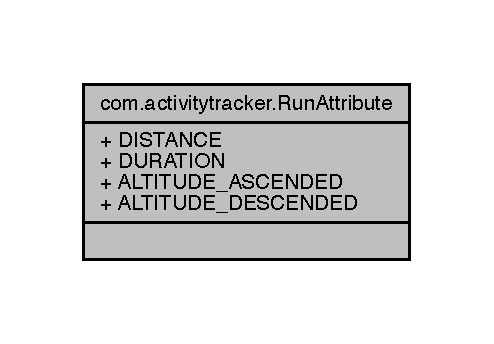
\includegraphics[width=237pt]{enumcom_1_1activitytracker_1_1_run_attribute__coll__graph}
\end{center}
\end{figure}
\subsection*{Public Attributes}
\begin{DoxyCompactItemize}
\item 
\mbox{\hyperlink{enumcom_1_1activitytracker_1_1_run_attribute_a90ee541e68e458a0bb3f5ea45fd46ec0}{D\+I\+S\+T\+A\+N\+CE}}
\item 
\mbox{\hyperlink{enumcom_1_1activitytracker_1_1_run_attribute_a7adf133b2a62f1f99ffc2adfb7097ec9}{D\+U\+R\+A\+T\+I\+ON}}
\item 
\mbox{\hyperlink{enumcom_1_1activitytracker_1_1_run_attribute_abcfe85bf48187d67842a0525c1bcc0af}{A\+L\+T\+I\+T\+U\+D\+E\+\_\+\+A\+S\+C\+E\+N\+D\+ED}}
\item 
\mbox{\hyperlink{enumcom_1_1activitytracker_1_1_run_attribute_a337a68867cfdb8ec7a17c318ad8b216b}{A\+L\+T\+I\+T\+U\+D\+E\+\_\+\+D\+E\+S\+C\+E\+N\+D\+ED}}
\item 
\mbox{\hyperlink{enumcom_1_1activitytracker_1_1_run_attribute_a43fc543df9ec6dfaac73a5030abfafc4}{S\+P\+E\+ED}}
\end{DoxyCompactItemize}


\subsection{Detailed Description}
This enumeration type is used to specify the behaviour of generalized methods, particularly in the \mbox{\hyperlink{classcom_1_1activitytracker_1_1_d_b_manager}{D\+B\+Manager}} class. 

Definition at line 6 of file Run\+Attribute.\+java.



\subsection{Member Data Documentation}
\mbox{\Hypertarget{enumcom_1_1activitytracker_1_1_run_attribute_abcfe85bf48187d67842a0525c1bcc0af}\label{enumcom_1_1activitytracker_1_1_run_attribute_abcfe85bf48187d67842a0525c1bcc0af}} 
\index{com\+::activitytracker\+::\+Run\+Attribute@{com\+::activitytracker\+::\+Run\+Attribute}!A\+L\+T\+I\+T\+U\+D\+E\+\_\+\+A\+S\+C\+E\+N\+D\+ED@{A\+L\+T\+I\+T\+U\+D\+E\+\_\+\+A\+S\+C\+E\+N\+D\+ED}}
\index{A\+L\+T\+I\+T\+U\+D\+E\+\_\+\+A\+S\+C\+E\+N\+D\+ED@{A\+L\+T\+I\+T\+U\+D\+E\+\_\+\+A\+S\+C\+E\+N\+D\+ED}!com\+::activitytracker\+::\+Run\+Attribute@{com\+::activitytracker\+::\+Run\+Attribute}}
\subsubsection{\texorpdfstring{A\+L\+T\+I\+T\+U\+D\+E\+\_\+\+A\+S\+C\+E\+N\+D\+ED}{ALTITUDE\_ASCENDED}}
{\footnotesize\ttfamily com.\+activitytracker.\+Run\+Attribute.\+A\+L\+T\+I\+T\+U\+D\+E\+\_\+\+A\+S\+C\+E\+N\+D\+ED}

The cumulative altitude (in metres) that the user has climbed throughout their run.

Used in \mbox{\hyperlink{classcom_1_1activitytracker_1_1_d_b_manager_a666452f1e5862f90c06b0beb9a9fcfdd}{D\+B\+Manager\+::get\+Run\+Float\+Attribute}} to specify that ascended altitude should be returned and Run\+Stats\+::compute\+Mean(). 

Definition at line 27 of file Run\+Attribute.\+java.

\mbox{\Hypertarget{enumcom_1_1activitytracker_1_1_run_attribute_a337a68867cfdb8ec7a17c318ad8b216b}\label{enumcom_1_1activitytracker_1_1_run_attribute_a337a68867cfdb8ec7a17c318ad8b216b}} 
\index{com\+::activitytracker\+::\+Run\+Attribute@{com\+::activitytracker\+::\+Run\+Attribute}!A\+L\+T\+I\+T\+U\+D\+E\+\_\+\+D\+E\+S\+C\+E\+N\+D\+ED@{A\+L\+T\+I\+T\+U\+D\+E\+\_\+\+D\+E\+S\+C\+E\+N\+D\+ED}}
\index{A\+L\+T\+I\+T\+U\+D\+E\+\_\+\+D\+E\+S\+C\+E\+N\+D\+ED@{A\+L\+T\+I\+T\+U\+D\+E\+\_\+\+D\+E\+S\+C\+E\+N\+D\+ED}!com\+::activitytracker\+::\+Run\+Attribute@{com\+::activitytracker\+::\+Run\+Attribute}}
\subsubsection{\texorpdfstring{A\+L\+T\+I\+T\+U\+D\+E\+\_\+\+D\+E\+S\+C\+E\+N\+D\+ED}{ALTITUDE\_DESCENDED}}
{\footnotesize\ttfamily com.\+activitytracker.\+Run\+Attribute.\+A\+L\+T\+I\+T\+U\+D\+E\+\_\+\+D\+E\+S\+C\+E\+N\+D\+ED}

The cumulative altitude (in metres) that the user has descended throughout their run.

Used in \mbox{\hyperlink{classcom_1_1activitytracker_1_1_d_b_manager_a666452f1e5862f90c06b0beb9a9fcfdd}{D\+B\+Manager\+::get\+Run\+Float\+Attribute}} to specify that descended altitude should be returned and Run\+Stats\+::compute\+Mean(). 

Definition at line 34 of file Run\+Attribute.\+java.

\mbox{\Hypertarget{enumcom_1_1activitytracker_1_1_run_attribute_a90ee541e68e458a0bb3f5ea45fd46ec0}\label{enumcom_1_1activitytracker_1_1_run_attribute_a90ee541e68e458a0bb3f5ea45fd46ec0}} 
\index{com\+::activitytracker\+::\+Run\+Attribute@{com\+::activitytracker\+::\+Run\+Attribute}!D\+I\+S\+T\+A\+N\+CE@{D\+I\+S\+T\+A\+N\+CE}}
\index{D\+I\+S\+T\+A\+N\+CE@{D\+I\+S\+T\+A\+N\+CE}!com\+::activitytracker\+::\+Run\+Attribute@{com\+::activitytracker\+::\+Run\+Attribute}}
\subsubsection{\texorpdfstring{D\+I\+S\+T\+A\+N\+CE}{DISTANCE}}
{\footnotesize\ttfamily com.\+activitytracker.\+Run\+Attribute.\+D\+I\+S\+T\+A\+N\+CE}

The cumulative distance the user has run (in metres).

Used in \mbox{\hyperlink{classcom_1_1activitytracker_1_1_d_b_manager_a666452f1e5862f90c06b0beb9a9fcfdd}{D\+B\+Manager\+::get\+Run\+Float\+Attribute}} to specify that distance should be returned and Run\+Stats\+::compute\+Mean(). 

Definition at line 13 of file Run\+Attribute.\+java.

\mbox{\Hypertarget{enumcom_1_1activitytracker_1_1_run_attribute_a7adf133b2a62f1f99ffc2adfb7097ec9}\label{enumcom_1_1activitytracker_1_1_run_attribute_a7adf133b2a62f1f99ffc2adfb7097ec9}} 
\index{com\+::activitytracker\+::\+Run\+Attribute@{com\+::activitytracker\+::\+Run\+Attribute}!D\+U\+R\+A\+T\+I\+ON@{D\+U\+R\+A\+T\+I\+ON}}
\index{D\+U\+R\+A\+T\+I\+ON@{D\+U\+R\+A\+T\+I\+ON}!com\+::activitytracker\+::\+Run\+Attribute@{com\+::activitytracker\+::\+Run\+Attribute}}
\subsubsection{\texorpdfstring{D\+U\+R\+A\+T\+I\+ON}{DURATION}}
{\footnotesize\ttfamily com.\+activitytracker.\+Run\+Attribute.\+D\+U\+R\+A\+T\+I\+ON}

The duration of the user\textquotesingle{}s run (in seconds).

Used in \mbox{\hyperlink{classcom_1_1activitytracker_1_1_d_b_manager_a666452f1e5862f90c06b0beb9a9fcfdd}{D\+B\+Manager\+::get\+Run\+Float\+Attribute}} to specify that duration should be returned and Run\+Stats\+::compute\+Mean(). 

Definition at line 20 of file Run\+Attribute.\+java.

\mbox{\Hypertarget{enumcom_1_1activitytracker_1_1_run_attribute_a43fc543df9ec6dfaac73a5030abfafc4}\label{enumcom_1_1activitytracker_1_1_run_attribute_a43fc543df9ec6dfaac73a5030abfafc4}} 
\index{com\+::activitytracker\+::\+Run\+Attribute@{com\+::activitytracker\+::\+Run\+Attribute}!S\+P\+E\+ED@{S\+P\+E\+ED}}
\index{S\+P\+E\+ED@{S\+P\+E\+ED}!com\+::activitytracker\+::\+Run\+Attribute@{com\+::activitytracker\+::\+Run\+Attribute}}
\subsubsection{\texorpdfstring{S\+P\+E\+ED}{SPEED}}
{\footnotesize\ttfamily com.\+activitytracker.\+Run\+Attribute.\+S\+P\+E\+ED}

The average speed the user ran.

Used in Run\+Stats\+::compute\+Mean(). 

Definition at line 40 of file Run\+Attribute.\+java.



The documentation for this enum was generated from the following file\+:\begin{DoxyCompactItemize}
\item 
app/src/com/activitytracker/\mbox{\hyperlink{_run_attribute_8java}{Run\+Attribute.\+java}}\end{DoxyCompactItemize}

\hypertarget{classcom_1_1activitytracker_1_1_secure_string}{}\section{com.\+activitytracker.\+Secure\+String Class Reference}
\label{classcom_1_1activitytracker_1_1_secure_string}\index{com.\+activitytracker.\+Secure\+String@{com.\+activitytracker.\+Secure\+String}}


Collaboration diagram for com.\+activitytracker.\+Secure\+String\+:
\nopagebreak
\begin{figure}[H]
\begin{center}
\leavevmode
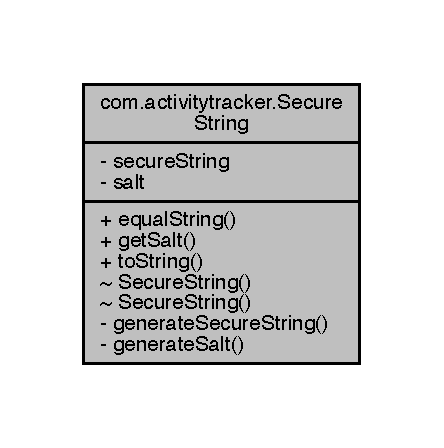
\includegraphics[width=213pt]{classcom_1_1activitytracker_1_1_secure_string__coll__graph}
\end{center}
\end{figure}
\subsection*{Public Member Functions}
\begin{DoxyCompactItemize}
\item 
boolean \mbox{\hyperlink{classcom_1_1activitytracker_1_1_secure_string_a8b5c3cac74b22ff0eb3c43a7ebd980f5}{equal\+String}} (final String other)
\item 
byte \mbox{[}$\,$\mbox{]} \mbox{\hyperlink{classcom_1_1activitytracker_1_1_secure_string_ab5369653852da122aba874f35cbda9a5}{get\+Salt}} ()
\item 
String \mbox{\hyperlink{classcom_1_1activitytracker_1_1_secure_string_aef531e12618c5c147adc52fda0d4add8}{to\+String}} ()
\end{DoxyCompactItemize}
\subsection*{Package Functions}
\begin{DoxyCompactItemize}
\item 
\mbox{\hyperlink{classcom_1_1activitytracker_1_1_secure_string_a889fcbf0c1f771962ac81886f49e389e}{Secure\+String}} (final String plaintext)
\item 
\mbox{\hyperlink{classcom_1_1activitytracker_1_1_secure_string_a04c2f0677ecd9af147428976a11c85e2}{Secure\+String}} (final String plaintext, final byte\mbox{[}$\,$\mbox{]} \mbox{\hyperlink{classcom_1_1activitytracker_1_1_secure_string_a8549ead1f186ff0c2520818b03d1cc21}{salt}})
\end{DoxyCompactItemize}
\subsection*{Private Member Functions}
\begin{DoxyCompactItemize}
\item 
String \mbox{\hyperlink{classcom_1_1activitytracker_1_1_secure_string_aa2521591ab15fb4c5a2461c04b08320f}{generate\+Secure\+String}} (final String str\+To\+Secure, final byte\mbox{[}$\,$\mbox{]} \mbox{\hyperlink{classcom_1_1activitytracker_1_1_secure_string_a8549ead1f186ff0c2520818b03d1cc21}{salt}})
\end{DoxyCompactItemize}
\subsection*{Static Private Member Functions}
\begin{DoxyCompactItemize}
\item 
static byte \mbox{[}$\,$\mbox{]} \mbox{\hyperlink{classcom_1_1activitytracker_1_1_secure_string_a1907ad109bb5e64291fabd3ff459ef49}{generate\+Salt}} ()  throws No\+Such\+Algorithm\+Exception 
\end{DoxyCompactItemize}
\subsection*{Private Attributes}
\begin{DoxyCompactItemize}
\item 
String \mbox{\hyperlink{classcom_1_1activitytracker_1_1_secure_string_a1448f7b8865c6c57cc7218662ee7f1ee}{secure\+String}}
\item 
byte \mbox{[}$\,$\mbox{]} \mbox{\hyperlink{classcom_1_1activitytracker_1_1_secure_string_a8549ead1f186ff0c2520818b03d1cc21}{salt}}
\end{DoxyCompactItemize}


\subsection{Detailed Description}
This class is used to securely store sensitive string-\/like information such as user passwords. 

Definition at line 10 of file Secure\+String.\+java.



\subsection{Constructor \& Destructor Documentation}
\mbox{\Hypertarget{classcom_1_1activitytracker_1_1_secure_string_a889fcbf0c1f771962ac81886f49e389e}\label{classcom_1_1activitytracker_1_1_secure_string_a889fcbf0c1f771962ac81886f49e389e}} 
\index{com\+::activitytracker\+::\+Secure\+String@{com\+::activitytracker\+::\+Secure\+String}!Secure\+String@{Secure\+String}}
\index{Secure\+String@{Secure\+String}!com\+::activitytracker\+::\+Secure\+String@{com\+::activitytracker\+::\+Secure\+String}}
\subsubsection{\texorpdfstring{Secure\+String()}{SecureString()}\hspace{0.1cm}{\footnotesize\ttfamily [1/2]}}
{\footnotesize\ttfamily com.\+activitytracker.\+Secure\+String.\+Secure\+String (\begin{DoxyParamCaption}\item[{final String}]{plaintext }\end{DoxyParamCaption})\hspace{0.3cm}{\ttfamily [package]}}

The \mbox{\hyperlink{classcom_1_1activitytracker_1_1_secure_string_a889fcbf0c1f771962ac81886f49e389e}{Secure\+String()}} constructor takes as an argument a plain text string, encrypts it, and stores the encrypted string in the variable \mbox{\hyperlink{classcom_1_1activitytracker_1_1_secure_string_a1448f7b8865c6c57cc7218662ee7f1ee}{Secure\+String\+::secure\+String}}.

Salt is generated using \mbox{\hyperlink{classcom_1_1activitytracker_1_1_secure_string_a1907ad109bb5e64291fabd3ff459ef49}{Secure\+String\+::generate\+Salt()}}.


\begin{DoxyParams}{Parameters}
{\em plaintext} & The string to be encrypted. May contain sensitive information. \\
\hline
\end{DoxyParams}


Definition at line 29 of file Secure\+String.\+java.


\begin{DoxyCode}
29                                          \{
30 
31         \textcolor{keywordflow}{try} \{
32             this.\mbox{\hyperlink{classcom_1_1activitytracker_1_1_secure_string_a8549ead1f186ff0c2520818b03d1cc21}{salt}} = \mbox{\hyperlink{classcom_1_1activitytracker_1_1_secure_string_a1907ad109bb5e64291fabd3ff459ef49}{generateSalt}}();
33         \}
34         \textcolor{keywordflow}{catch} (\textcolor{keyword}{final} NoSuchAlgorithmException e) \{
35             System.err.println(e.getMessage());
36         \}
37         this.\mbox{\hyperlink{classcom_1_1activitytracker_1_1_secure_string_a1448f7b8865c6c57cc7218662ee7f1ee}{secureString}} = \mbox{\hyperlink{classcom_1_1activitytracker_1_1_secure_string_aa2521591ab15fb4c5a2461c04b08320f}{generateSecureString}}(plaintext, this.
      \mbox{\hyperlink{classcom_1_1activitytracker_1_1_secure_string_a8549ead1f186ff0c2520818b03d1cc21}{salt}});
38 
39     \}
\end{DoxyCode}
\mbox{\Hypertarget{classcom_1_1activitytracker_1_1_secure_string_a04c2f0677ecd9af147428976a11c85e2}\label{classcom_1_1activitytracker_1_1_secure_string_a04c2f0677ecd9af147428976a11c85e2}} 
\index{com\+::activitytracker\+::\+Secure\+String@{com\+::activitytracker\+::\+Secure\+String}!Secure\+String@{Secure\+String}}
\index{Secure\+String@{Secure\+String}!com\+::activitytracker\+::\+Secure\+String@{com\+::activitytracker\+::\+Secure\+String}}
\subsubsection{\texorpdfstring{Secure\+String()}{SecureString()}\hspace{0.1cm}{\footnotesize\ttfamily [2/2]}}
{\footnotesize\ttfamily com.\+activitytracker.\+Secure\+String.\+Secure\+String (\begin{DoxyParamCaption}\item[{final String}]{plaintext,  }\item[{final byte \mbox{[}$\,$\mbox{]}}]{salt }\end{DoxyParamCaption})\hspace{0.3cm}{\ttfamily [package]}}

The \mbox{\hyperlink{classcom_1_1activitytracker_1_1_secure_string_a889fcbf0c1f771962ac81886f49e389e}{Secure\+String()}} constructor takes as an argument a plain text string and a previously-\/generated salt, encrypts the plain text string with the provided salt, and stores the encrypted string in the variable \mbox{\hyperlink{classcom_1_1activitytracker_1_1_secure_string_a1448f7b8865c6c57cc7218662ee7f1ee}{Secure\+String\+::secure\+String}}.


\begin{DoxyParams}{Parameters}
{\em plaintext} & The string to be encrypted. May contain sensitive information. \\
\hline
{\em salt} & Salt that is used to encrypt {\itshape plaintext}. This parameter is used whenever we wish to encrypt using a previously-\/generated salt for the purpose of encrypted string comparison. \\
\hline
\end{DoxyParams}


Definition at line 50 of file Secure\+String.\+java.


\begin{DoxyCode}
50                                                             \{
51 
52         this.\mbox{\hyperlink{classcom_1_1activitytracker_1_1_secure_string_a8549ead1f186ff0c2520818b03d1cc21}{salt}} = \mbox{\hyperlink{classcom_1_1activitytracker_1_1_secure_string_a8549ead1f186ff0c2520818b03d1cc21}{salt}};
53         this.\mbox{\hyperlink{classcom_1_1activitytracker_1_1_secure_string_a1448f7b8865c6c57cc7218662ee7f1ee}{secureString}} = \mbox{\hyperlink{classcom_1_1activitytracker_1_1_secure_string_aa2521591ab15fb4c5a2461c04b08320f}{generateSecureString}}(plaintext, 
      \mbox{\hyperlink{classcom_1_1activitytracker_1_1_secure_string_a8549ead1f186ff0c2520818b03d1cc21}{salt}});
54 
55     \}
\end{DoxyCode}


\subsection{Member Function Documentation}
\mbox{\Hypertarget{classcom_1_1activitytracker_1_1_secure_string_a8b5c3cac74b22ff0eb3c43a7ebd980f5}\label{classcom_1_1activitytracker_1_1_secure_string_a8b5c3cac74b22ff0eb3c43a7ebd980f5}} 
\index{com\+::activitytracker\+::\+Secure\+String@{com\+::activitytracker\+::\+Secure\+String}!equal\+String@{equal\+String}}
\index{equal\+String@{equal\+String}!com\+::activitytracker\+::\+Secure\+String@{com\+::activitytracker\+::\+Secure\+String}}
\subsubsection{\texorpdfstring{equal\+String()}{equalString()}}
{\footnotesize\ttfamily boolean com.\+activitytracker.\+Secure\+String.\+equal\+String (\begin{DoxyParamCaption}\item[{final String}]{other }\end{DoxyParamCaption})}

Compares the secure string to the {\itshape other} parameter for equality.

This method will likely be used to authenticate a user from a password hash existing in the database.


\begin{DoxyParams}{Parameters}
{\em other} & A (previously encrypted) string with with we compare \mbox{\hyperlink{classcom_1_1activitytracker_1_1_secure_string_a1448f7b8865c6c57cc7218662ee7f1ee}{Secure\+String\+::secure\+String}}.\\
\hline
\end{DoxyParams}
\begin{DoxyReturn}{Returns}
This method returns True if the hashes of both strings are the same, and False otherwise. 
\end{DoxyReturn}


Definition at line 66 of file Secure\+String.\+java.


\begin{DoxyCode}
66                                                    \{
67 
68         \textcolor{keywordflow}{return} this.\mbox{\hyperlink{classcom_1_1activitytracker_1_1_secure_string_a1448f7b8865c6c57cc7218662ee7f1ee}{secureString}}.equals(other);
69 
70     \}
\end{DoxyCode}
\mbox{\Hypertarget{classcom_1_1activitytracker_1_1_secure_string_a1907ad109bb5e64291fabd3ff459ef49}\label{classcom_1_1activitytracker_1_1_secure_string_a1907ad109bb5e64291fabd3ff459ef49}} 
\index{com\+::activitytracker\+::\+Secure\+String@{com\+::activitytracker\+::\+Secure\+String}!generate\+Salt@{generate\+Salt}}
\index{generate\+Salt@{generate\+Salt}!com\+::activitytracker\+::\+Secure\+String@{com\+::activitytracker\+::\+Secure\+String}}
\subsubsection{\texorpdfstring{generate\+Salt()}{generateSalt()}}
{\footnotesize\ttfamily static byte \mbox{[}$\,$\mbox{]} com.\+activitytracker.\+Secure\+String.\+generate\+Salt (\begin{DoxyParamCaption}{ }\end{DoxyParamCaption}) throws No\+Such\+Algorithm\+Exception\hspace{0.3cm}{\ttfamily [static]}, {\ttfamily [private]}}

This method generates salt for encryption of a plain text string.

\begin{DoxyReturn}{Returns}
Returns a byte array of length sixteen (16) containing the encryption salt.
\end{DoxyReturn}

\begin{DoxyExceptions}{Exceptions}
{\em No\+Such\+Algorithm\+Exception} & Required as {\itshape Secure\+Random.\+get\+Instace()} may throw this exception and we would like the invoking method to decide how to handle it rather than catching and dismissing it here. \\
\hline
\end{DoxyExceptions}


Definition at line 83 of file Secure\+String.\+java.


\begin{DoxyCode}
83                                                                          \{
84         SecureRandom sr = SecureRandom.getInstance(\textcolor{stringliteral}{"SHA1PRNG"});
85         byte[] \mbox{\hyperlink{classcom_1_1activitytracker_1_1_secure_string_a8549ead1f186ff0c2520818b03d1cc21}{salt}} = \textcolor{keyword}{new} byte[16];
86         sr.nextBytes(\mbox{\hyperlink{classcom_1_1activitytracker_1_1_secure_string_a8549ead1f186ff0c2520818b03d1cc21}{salt}});
87         \textcolor{keywordflow}{return} \mbox{\hyperlink{classcom_1_1activitytracker_1_1_secure_string_a8549ead1f186ff0c2520818b03d1cc21}{salt}};
88     \}
\end{DoxyCode}
\mbox{\Hypertarget{classcom_1_1activitytracker_1_1_secure_string_aa2521591ab15fb4c5a2461c04b08320f}\label{classcom_1_1activitytracker_1_1_secure_string_aa2521591ab15fb4c5a2461c04b08320f}} 
\index{com\+::activitytracker\+::\+Secure\+String@{com\+::activitytracker\+::\+Secure\+String}!generate\+Secure\+String@{generate\+Secure\+String}}
\index{generate\+Secure\+String@{generate\+Secure\+String}!com\+::activitytracker\+::\+Secure\+String@{com\+::activitytracker\+::\+Secure\+String}}
\subsubsection{\texorpdfstring{generate\+Secure\+String()}{generateSecureString()}}
{\footnotesize\ttfamily String com.\+activitytracker.\+Secure\+String.\+generate\+Secure\+String (\begin{DoxyParamCaption}\item[{final String}]{str\+To\+Secure,  }\item[{final byte \mbox{[}$\,$\mbox{]}}]{salt }\end{DoxyParamCaption})\hspace{0.3cm}{\ttfamily [private]}}

Encrypt string and return secure version.

Due to the importance of securely storing passwords, a \char`\"{}tried and true\char`\"{} method for encrypting passwords found at \href{https://howtodoinjava.com/security/how-to-generate-secure-password-hash-md5-sha-pbkdf2-bcrypt-examples/}{\tt this link} has been used.


\begin{DoxyParams}{Parameters}
{\em str\+To\+Secure} & The plain text string we wish to encrypt. \\
\hline
{\em salt} & The salt with which we will encrypt {\itshape str\+To\+Secure}.\\
\hline
\end{DoxyParams}
\begin{DoxyReturn}{Returns}
This private method returns the encrypted string to the \mbox{\hyperlink{classcom_1_1activitytracker_1_1_secure_string_a889fcbf0c1f771962ac81886f49e389e}{Secure\+String()}} constructor. 
\end{DoxyReturn}


Definition at line 102 of file Secure\+String.\+java.


\begin{DoxyCode}
102                                                                                      \{
103         String generatedPassword = null;
104         \textcolor{keywordflow}{try} \{
105             MessageDigest md = MessageDigest.getInstance(\textcolor{stringliteral}{"SHA-512"});
106             md.update(\mbox{\hyperlink{classcom_1_1activitytracker_1_1_secure_string_a8549ead1f186ff0c2520818b03d1cc21}{salt}});
107             byte[] strBytes = md.digest(strToSecure.getBytes());
108             StringBuilder sb = \textcolor{keyword}{new} StringBuilder();
109             \textcolor{keywordflow}{for} (\textcolor{keywordtype}{int} i = 0; i < strBytes.length; i++) \{
110                 sb.append(Integer.toString((strBytes[i] & 0xff) + 0x100, 16).substring(1));
111             \}
112             generatedPassword = sb.toString();
113         \}
114         \textcolor{keywordflow}{catch} (\textcolor{keyword}{final} NoSuchAlgorithmException e) \{
115             System.err.println(e.getMessage());
116         \}
117         \textcolor{keywordflow}{return} generatedPassword;
118     \}
\end{DoxyCode}
\mbox{\Hypertarget{classcom_1_1activitytracker_1_1_secure_string_ab5369653852da122aba874f35cbda9a5}\label{classcom_1_1activitytracker_1_1_secure_string_ab5369653852da122aba874f35cbda9a5}} 
\index{com\+::activitytracker\+::\+Secure\+String@{com\+::activitytracker\+::\+Secure\+String}!get\+Salt@{get\+Salt}}
\index{get\+Salt@{get\+Salt}!com\+::activitytracker\+::\+Secure\+String@{com\+::activitytracker\+::\+Secure\+String}}
\subsubsection{\texorpdfstring{get\+Salt()}{getSalt()}}
{\footnotesize\ttfamily byte \mbox{[}$\,$\mbox{]} com.\+activitytracker.\+Secure\+String.\+get\+Salt (\begin{DoxyParamCaption}{ }\end{DoxyParamCaption})}

\begin{DoxyReturn}{Returns}
Returns the byte array-\/type salt used to encrypt the text given to the object\textquotesingle{}s constructor. 
\end{DoxyReturn}


Definition at line 123 of file Secure\+String.\+java.


\begin{DoxyCode}
123                             \{
124         \textcolor{keywordflow}{return} this.\mbox{\hyperlink{classcom_1_1activitytracker_1_1_secure_string_a8549ead1f186ff0c2520818b03d1cc21}{salt}};
125     \}
\end{DoxyCode}
\mbox{\Hypertarget{classcom_1_1activitytracker_1_1_secure_string_aef531e12618c5c147adc52fda0d4add8}\label{classcom_1_1activitytracker_1_1_secure_string_aef531e12618c5c147adc52fda0d4add8}} 
\index{com\+::activitytracker\+::\+Secure\+String@{com\+::activitytracker\+::\+Secure\+String}!to\+String@{to\+String}}
\index{to\+String@{to\+String}!com\+::activitytracker\+::\+Secure\+String@{com\+::activitytracker\+::\+Secure\+String}}
\subsubsection{\texorpdfstring{to\+String()}{toString()}}
{\footnotesize\ttfamily String com.\+activitytracker.\+Secure\+String.\+to\+String (\begin{DoxyParamCaption}{ }\end{DoxyParamCaption})}

Overrided method to return the object as a Java String.

The encrypted string will be returned, though it should be noted for completeness that this is not a full representation of the object since the salt is crucial in arriving at \mbox{\hyperlink{classcom_1_1activitytracker_1_1_secure_string_a1448f7b8865c6c57cc7218662ee7f1ee}{Secure\+String\+::secure\+String}} being returned.

\begin{DoxyReturn}{Returns}
Returns the encrypted string. 
\end{DoxyReturn}


Definition at line 136 of file Secure\+String.\+java.


\begin{DoxyCode}
136                              \{
137         \textcolor{keywordflow}{return} this.\mbox{\hyperlink{classcom_1_1activitytracker_1_1_secure_string_a1448f7b8865c6c57cc7218662ee7f1ee}{secureString}};
138     \}
\end{DoxyCode}


\subsection{Member Data Documentation}
\mbox{\Hypertarget{classcom_1_1activitytracker_1_1_secure_string_a8549ead1f186ff0c2520818b03d1cc21}\label{classcom_1_1activitytracker_1_1_secure_string_a8549ead1f186ff0c2520818b03d1cc21}} 
\index{com\+::activitytracker\+::\+Secure\+String@{com\+::activitytracker\+::\+Secure\+String}!salt@{salt}}
\index{salt@{salt}!com\+::activitytracker\+::\+Secure\+String@{com\+::activitytracker\+::\+Secure\+String}}
\subsubsection{\texorpdfstring{salt}{salt}}
{\footnotesize\ttfamily byte \mbox{[}$\,$\mbox{]} com.\+activitytracker.\+Secure\+String.\+salt\hspace{0.3cm}{\ttfamily [private]}}

The salt that was used to encrypt the plain text string. 

Definition at line 19 of file Secure\+String.\+java.

\mbox{\Hypertarget{classcom_1_1activitytracker_1_1_secure_string_a1448f7b8865c6c57cc7218662ee7f1ee}\label{classcom_1_1activitytracker_1_1_secure_string_a1448f7b8865c6c57cc7218662ee7f1ee}} 
\index{com\+::activitytracker\+::\+Secure\+String@{com\+::activitytracker\+::\+Secure\+String}!secure\+String@{secure\+String}}
\index{secure\+String@{secure\+String}!com\+::activitytracker\+::\+Secure\+String@{com\+::activitytracker\+::\+Secure\+String}}
\subsubsection{\texorpdfstring{secure\+String}{secureString}}
{\footnotesize\ttfamily String com.\+activitytracker.\+Secure\+String.\+secure\+String\hspace{0.3cm}{\ttfamily [private]}}

The encrypted string. 

Definition at line 15 of file Secure\+String.\+java.



The documentation for this class was generated from the following file\+:\begin{DoxyCompactItemize}
\item 
app/src/com/activitytracker/\mbox{\hyperlink{_secure_string_8java}{Secure\+String.\+java}}\end{DoxyCompactItemize}

\hypertarget{enumcom_1_1activitytracker_1_1_user_1_1_sex}{}\section{com.\+activitytracker.\+User.\+Sex Enum Reference}
\label{enumcom_1_1activitytracker_1_1_user_1_1_sex}\index{com.\+activitytracker.\+User.\+Sex@{com.\+activitytracker.\+User.\+Sex}}
\subsection*{Public Attributes}
\begin{DoxyCompactItemize}
\item 
\mbox{\hyperlink{enumcom_1_1activitytracker_1_1_user_1_1_sex_ad3b626a38bd4615eb621d75b939f412d}{M\+A\+LE}}
\item 
\mbox{\hyperlink{enumcom_1_1activitytracker_1_1_user_1_1_sex_a5c22ece8a4df71ed5202cd492990a752}{F\+E\+M\+A\+LE}}
\end{DoxyCompactItemize}


\subsection{Detailed Description}
Used to represent whether the user is male or female. 

Definition at line 12 of file User.\+java.



\subsection{Member Data Documentation}
\mbox{\Hypertarget{enumcom_1_1activitytracker_1_1_user_1_1_sex_a5c22ece8a4df71ed5202cd492990a752}\label{enumcom_1_1activitytracker_1_1_user_1_1_sex_a5c22ece8a4df71ed5202cd492990a752}} 
\index{com\+::activitytracker\+::\+User\+::\+Sex@{com\+::activitytracker\+::\+User\+::\+Sex}!F\+E\+M\+A\+LE@{F\+E\+M\+A\+LE}}
\index{F\+E\+M\+A\+LE@{F\+E\+M\+A\+LE}!com\+::activitytracker\+::\+User\+::\+Sex@{com\+::activitytracker\+::\+User\+::\+Sex}}
\subsubsection{\texorpdfstring{F\+E\+M\+A\+LE}{FEMALE}}
{\footnotesize\ttfamily com.\+activitytracker.\+User.\+Sex.\+F\+E\+M\+A\+LE}

Used to represent that the user is female.

Recall from the source code included in \mbox{\hyperlink{classcom_1_1activitytracker_1_1_d_b_manager_a41df4600bb5901a26a4ea6a7108a70b9}{D\+B\+Manager\+::init()}} that sex is stored in the database using a data type of B\+I\+T(1). If the user is female, we store this in the database by populating this field with a {\itshape 0}. 

Definition at line 26 of file User.\+java.

\mbox{\Hypertarget{enumcom_1_1activitytracker_1_1_user_1_1_sex_ad3b626a38bd4615eb621d75b939f412d}\label{enumcom_1_1activitytracker_1_1_user_1_1_sex_ad3b626a38bd4615eb621d75b939f412d}} 
\index{com\+::activitytracker\+::\+User\+::\+Sex@{com\+::activitytracker\+::\+User\+::\+Sex}!M\+A\+LE@{M\+A\+LE}}
\index{M\+A\+LE@{M\+A\+LE}!com\+::activitytracker\+::\+User\+::\+Sex@{com\+::activitytracker\+::\+User\+::\+Sex}}
\subsubsection{\texorpdfstring{M\+A\+LE}{MALE}}
{\footnotesize\ttfamily com.\+activitytracker.\+User.\+Sex.\+M\+A\+LE}

Used to represent that the user is male.

Recall from the source code included in \mbox{\hyperlink{classcom_1_1activitytracker_1_1_d_b_manager_a41df4600bb5901a26a4ea6a7108a70b9}{D\+B\+Manager\+::init()}} that sex is stored in the database using a data type of B\+I\+T(1). If the user is female, we store this in the database by populating this field with a {\itshape 1}. 

Definition at line 19 of file User.\+java.



The documentation for this enum was generated from the following file\+:\begin{DoxyCompactItemize}
\item 
app/src/com/activitytracker/\mbox{\hyperlink{_user_8java}{User.\+java}}\end{DoxyCompactItemize}

\hypertarget{classcom_1_1activitytracker_1_1_user}{}\section{com.\+activitytracker.\+User Class Reference}
\label{classcom_1_1activitytracker_1_1_user}\index{com.\+activitytracker.\+User@{com.\+activitytracker.\+User}}


Collaboration diagram for com.\+activitytracker.\+User\+:
\nopagebreak
\begin{figure}[H]
\begin{center}
\leavevmode
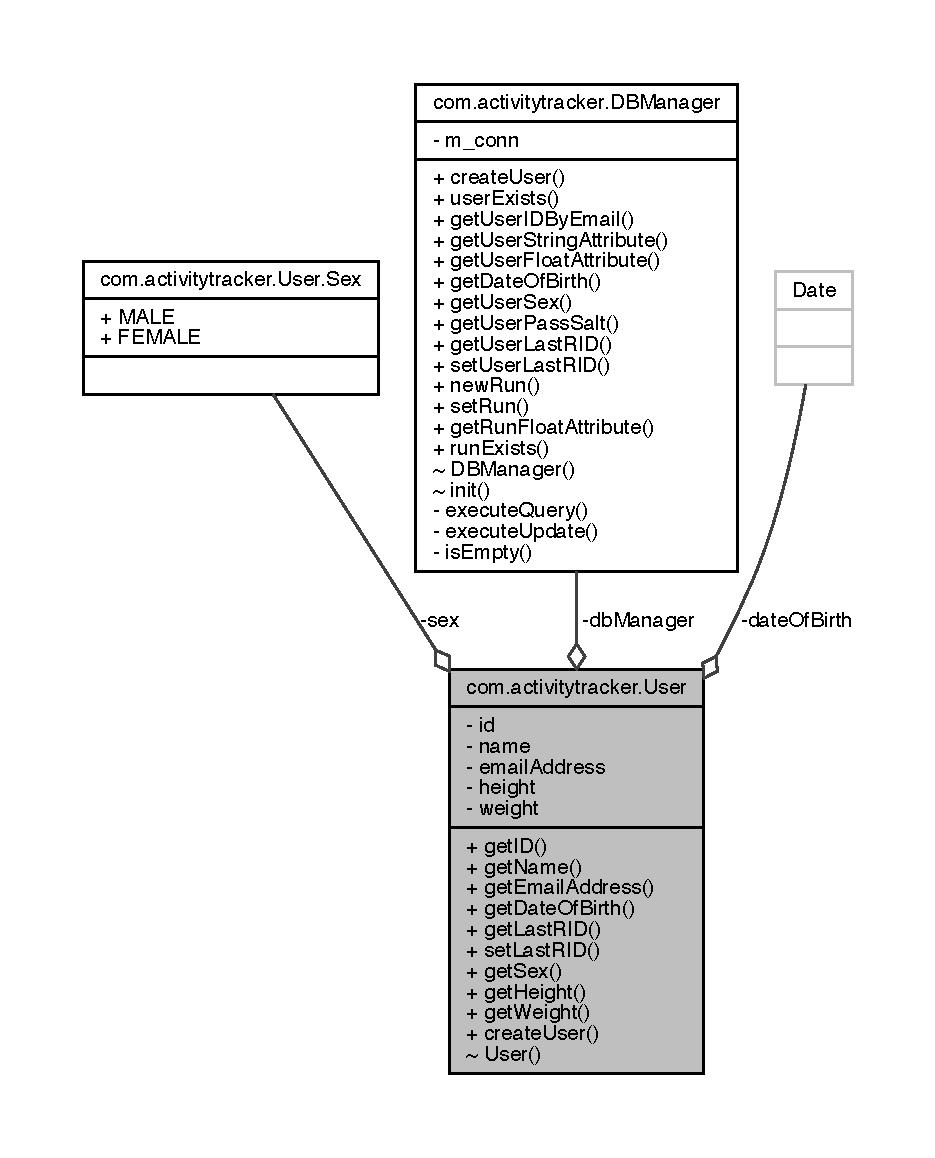
\includegraphics[width=350pt]{classcom_1_1activitytracker_1_1_user__coll__graph}
\end{center}
\end{figure}
\subsection*{Classes}
\begin{DoxyCompactItemize}
\item 
enum \mbox{\hyperlink{enumcom_1_1activitytracker_1_1_user_1_1_sex}{Sex}}
\end{DoxyCompactItemize}
\subsection*{Public Member Functions}
\begin{DoxyCompactItemize}
\item 
int \mbox{\hyperlink{classcom_1_1activitytracker_1_1_user_a967ae64a7818e9e532ad6d361650d8e6}{get\+ID}} ()
\item 
String \mbox{\hyperlink{classcom_1_1activitytracker_1_1_user_a6b39e49a1e49279035fd61a667d14f64}{get\+Name}} ()
\item 
String \mbox{\hyperlink{classcom_1_1activitytracker_1_1_user_a79d69ca90216e0552ac4cae9778ea40d}{get\+Email\+Address}} ()
\item 
Date \mbox{\hyperlink{classcom_1_1activitytracker_1_1_user_a40da04454cea10bb5c6e6125a7a9cf64}{get\+Date\+Of\+Birth}} ()
\item 
int \mbox{\hyperlink{classcom_1_1activitytracker_1_1_user_a7040d0d696d79f9592eec6ac507de3c7}{get\+Last\+R\+ID}} ()
\item 
void \mbox{\hyperlink{classcom_1_1activitytracker_1_1_user_a9e91c79596a9a4dfda7b3453b61ff8d2}{set\+Last\+R\+ID}} (final int r\+ID)
\item 
\mbox{\hyperlink{enumcom_1_1activitytracker_1_1_user_1_1_sex}{Sex}} \mbox{\hyperlink{classcom_1_1activitytracker_1_1_user_ac184fdb794730df3fedf3b147283a5fd}{get\+Sex}} ()
\item 
float \mbox{\hyperlink{classcom_1_1activitytracker_1_1_user_a2a80ab659d02a07176b1793354131c00}{get\+Height}} ()
\item 
float \mbox{\hyperlink{classcom_1_1activitytracker_1_1_user_ad15d7b4f96adb6d1a14054bf3eb7e4e0}{get\+Weight}} ()
\end{DoxyCompactItemize}
\subsection*{Static Public Member Functions}
\begin{DoxyCompactItemize}
\item 
static void \mbox{\hyperlink{classcom_1_1activitytracker_1_1_user_ab9d405e0fc6916bbf4836ce6ab762bea}{create\+User}} (final \mbox{\hyperlink{classcom_1_1activitytracker_1_1_d_b_manager}{D\+B\+Manager}} \mbox{\hyperlink{classcom_1_1activitytracker_1_1_user_a8c8b36433447a235f2b4940b92e839c1}{db\+Manager}}, final String \mbox{\hyperlink{classcom_1_1activitytracker_1_1_user_a49bfb4c8ebf8b7a377df01b5f0b2d7bc}{name}}, final String \mbox{\hyperlink{classcom_1_1activitytracker_1_1_user_ac2fdb9a858d0295e52c5f8bc179e3137}{email\+Address}}, final int D\+O\+B\+Year, final int D\+O\+B\+Month, final int D\+O\+B\+Day, final User.\+Sex \mbox{\hyperlink{classcom_1_1activitytracker_1_1_user_adcbddd2e965af4e227f7cf0582a3e13d}{sex}}, final float \mbox{\hyperlink{classcom_1_1activitytracker_1_1_user_a83cdfe6f520a4e18e8710e8e11f8c3d6}{height}}, final float \mbox{\hyperlink{classcom_1_1activitytracker_1_1_user_a8a30c6c08983e513b462bcc035434c9e}{weight}}, final String plaintext\+Password)
\end{DoxyCompactItemize}
\subsection*{Package Functions}
\begin{DoxyCompactItemize}
\item 
\mbox{\hyperlink{classcom_1_1activitytracker_1_1_user_ae9f2a2555aa41e80ade28223907e01ab}{User}} (final \mbox{\hyperlink{classcom_1_1activitytracker_1_1_d_b_manager}{D\+B\+Manager}} \mbox{\hyperlink{classcom_1_1activitytracker_1_1_user_a8c8b36433447a235f2b4940b92e839c1}{db\+Manager}}, final String \mbox{\hyperlink{classcom_1_1activitytracker_1_1_user_ac2fdb9a858d0295e52c5f8bc179e3137}{email\+Address}}, final String plaintext\+Password)  throws Authentication\+Exception
\end{DoxyCompactItemize}
\subsection*{Private Attributes}
\begin{DoxyCompactItemize}
\item 
int \mbox{\hyperlink{classcom_1_1activitytracker_1_1_user_adc05319380c2cbb37477ab5aab86317c}{id}}
\item 
String \mbox{\hyperlink{classcom_1_1activitytracker_1_1_user_a49bfb4c8ebf8b7a377df01b5f0b2d7bc}{name}}
\item 
String \mbox{\hyperlink{classcom_1_1activitytracker_1_1_user_ac2fdb9a858d0295e52c5f8bc179e3137}{email\+Address}}
\item 
Date \mbox{\hyperlink{classcom_1_1activitytracker_1_1_user_a40b0d4ce16246066c0e948edef864d94}{date\+Of\+Birth}}
\item 
\mbox{\hyperlink{enumcom_1_1activitytracker_1_1_user_1_1_sex}{Sex}} \mbox{\hyperlink{classcom_1_1activitytracker_1_1_user_adcbddd2e965af4e227f7cf0582a3e13d}{sex}}
\item 
float \mbox{\hyperlink{classcom_1_1activitytracker_1_1_user_a83cdfe6f520a4e18e8710e8e11f8c3d6}{height}}
\item 
float \mbox{\hyperlink{classcom_1_1activitytracker_1_1_user_a8a30c6c08983e513b462bcc035434c9e}{weight}}
\item 
\mbox{\hyperlink{classcom_1_1activitytracker_1_1_d_b_manager}{D\+B\+Manager}} \mbox{\hyperlink{classcom_1_1activitytracker_1_1_user_a8c8b36433447a235f2b4940b92e839c1}{db\+Manager}} = null
\end{DoxyCompactItemize}


\subsection{Detailed Description}


Definition at line 8 of file User.\+java.



\subsection{Constructor \& Destructor Documentation}
\mbox{\Hypertarget{classcom_1_1activitytracker_1_1_user_ae9f2a2555aa41e80ade28223907e01ab}\label{classcom_1_1activitytracker_1_1_user_ae9f2a2555aa41e80ade28223907e01ab}} 
\index{com\+::activitytracker\+::\+User@{com\+::activitytracker\+::\+User}!User@{User}}
\index{User@{User}!com\+::activitytracker\+::\+User@{com\+::activitytracker\+::\+User}}
\subsubsection{\texorpdfstring{User()}{User()}}
{\footnotesize\ttfamily com.\+activitytracker.\+User.\+User (\begin{DoxyParamCaption}\item[{final \mbox{\hyperlink{classcom_1_1activitytracker_1_1_d_b_manager}{D\+B\+Manager}}}]{db\+Manager,  }\item[{final String}]{email\+Address,  }\item[{final String}]{plaintext\+Password }\end{DoxyParamCaption}) throws Authentication\+Exception\hspace{0.3cm}{\ttfamily [package]}}



Definition at line 38 of file User.\+java.


\begin{DoxyCode}
38                                                                                                            
                        \{
39 
40         this.\mbox{\hyperlink{classcom_1_1activitytracker_1_1_user_a8c8b36433447a235f2b4940b92e839c1}{dbManager}} = \mbox{\hyperlink{classcom_1_1activitytracker_1_1_user_a8c8b36433447a235f2b4940b92e839c1}{dbManager}};
41         \textcolor{keywordflow}{if} (this.\mbox{\hyperlink{classcom_1_1activitytracker_1_1_user_a8c8b36433447a235f2b4940b92e839c1}{dbManager}}.\mbox{\hyperlink{classcom_1_1activitytracker_1_1_d_b_manager_af05d79f33ecf2920a67d1b9cf82c079f}{userExists}}(\mbox{\hyperlink{classcom_1_1activitytracker_1_1_user_ac2fdb9a858d0295e52c5f8bc179e3137}{emailAddress}})) \{
42 
43             this.\textcolor{keywordtype}{id} = \mbox{\hyperlink{classcom_1_1activitytracker_1_1_user_a8c8b36433447a235f2b4940b92e839c1}{dbManager}}.\mbox{\hyperlink{classcom_1_1activitytracker_1_1_d_b_manager_a195dcdeabdd00facb19d720976dd3f53}{getUserIDByEmail}}(
      \mbox{\hyperlink{classcom_1_1activitytracker_1_1_user_ac2fdb9a858d0295e52c5f8bc179e3137}{emailAddress}});
44 
45             String passHash = this.\mbox{\hyperlink{classcom_1_1activitytracker_1_1_user_a8c8b36433447a235f2b4940b92e839c1}{dbManager}}.\mbox{\hyperlink{classcom_1_1activitytracker_1_1_d_b_manager_a20f726c054d6c8a6fc3ce629d87f1114}{getUserStringAttribute}}(
      UserAttribute.PASSWORD, \textcolor{keyword}{this}.id);
46             byte[] passSalt = this.\mbox{\hyperlink{classcom_1_1activitytracker_1_1_user_a8c8b36433447a235f2b4940b92e839c1}{dbManager}}.\mbox{\hyperlink{classcom_1_1activitytracker_1_1_d_b_manager_aeab864b072cc08c0521e80ae1f459ca7}{getUserPassSalt}}(this.\textcolor{keywordtype}{id});
47 
48             SecureString candidatePassword = \textcolor{keyword}{new} SecureString(plaintextPassword, passSalt);
49 
50             \textcolor{keywordflow}{if} (candidatePassword.equalString(passHash)) \{
51 
52 
53                 this.\mbox{\hyperlink{classcom_1_1activitytracker_1_1_user_a49bfb4c8ebf8b7a377df01b5f0b2d7bc}{name}} = this.\mbox{\hyperlink{classcom_1_1activitytracker_1_1_user_a8c8b36433447a235f2b4940b92e839c1}{dbManager}}.\mbox{\hyperlink{classcom_1_1activitytracker_1_1_d_b_manager_a20f726c054d6c8a6fc3ce629d87f1114}{getUserStringAttribute}}(
      UserAttribute.NAME, \textcolor{keyword}{this}.id);
54 \textcolor{comment}{//                this.emailAddress = this.dbManager.getEmailAddress(this.id);}
55                 this.\mbox{\hyperlink{classcom_1_1activitytracker_1_1_user_ac2fdb9a858d0295e52c5f8bc179e3137}{emailAddress}} = \mbox{\hyperlink{classcom_1_1activitytracker_1_1_user_ac2fdb9a858d0295e52c5f8bc179e3137}{emailAddress}};
56                 this.\mbox{\hyperlink{classcom_1_1activitytracker_1_1_user_a40b0d4ce16246066c0e948edef864d94}{dateOfBirth}} = this.\mbox{\hyperlink{classcom_1_1activitytracker_1_1_user_a8c8b36433447a235f2b4940b92e839c1}{dbManager}}.
      \mbox{\hyperlink{classcom_1_1activitytracker_1_1_d_b_manager_a0576baf67b45c7d2d0ba369052e4404e}{getDateOfBirth}}(this.\textcolor{keywordtype}{id});
57                 this.\mbox{\hyperlink{classcom_1_1activitytracker_1_1_user_adcbddd2e965af4e227f7cf0582a3e13d}{sex}} = this.\mbox{\hyperlink{classcom_1_1activitytracker_1_1_user_a8c8b36433447a235f2b4940b92e839c1}{dbManager}}.\mbox{\hyperlink{classcom_1_1activitytracker_1_1_d_b_manager_a4e695c111b877cfd1d918602551f65a1}{getUserSex}}(this.\textcolor{keywordtype}{id});
58                 this.\mbox{\hyperlink{classcom_1_1activitytracker_1_1_user_a83cdfe6f520a4e18e8710e8e11f8c3d6}{height}} = this.\mbox{\hyperlink{classcom_1_1activitytracker_1_1_user_a8c8b36433447a235f2b4940b92e839c1}{dbManager}}.
      \mbox{\hyperlink{classcom_1_1activitytracker_1_1_d_b_manager_a98df66254bec4d74b29cfe468a9fc794}{getUserFloatAttribute}}(UserAttribute.HEIGHT, \textcolor{keyword}{this}.id);
59                 this.\mbox{\hyperlink{classcom_1_1activitytracker_1_1_user_a8a30c6c08983e513b462bcc035434c9e}{weight}} = this.\mbox{\hyperlink{classcom_1_1activitytracker_1_1_user_a8c8b36433447a235f2b4940b92e839c1}{dbManager}}.
      \mbox{\hyperlink{classcom_1_1activitytracker_1_1_d_b_manager_a98df66254bec4d74b29cfe468a9fc794}{getUserFloatAttribute}}(UserAttribute.WEIGHT, \textcolor{keyword}{this}.id);
60 
61                 System.out.println(\textcolor{stringliteral}{"Authentication succeeded for "} + this.\mbox{\hyperlink{classcom_1_1activitytracker_1_1_user_a49bfb4c8ebf8b7a377df01b5f0b2d7bc}{name}});
62 
63             \}
64             \textcolor{keywordflow}{else} \{
65 
66                 \textcolor{keywordflow}{throw} \textcolor{keyword}{new} AuthenticationException(\textcolor{stringliteral}{"Incorrect password."});
67 
68             \}
69         \}
70         \textcolor{keywordflow}{else} \{
71 
72             \textcolor{keywordflow}{throw} \textcolor{keyword}{new} NoSuchElementException(\textcolor{stringliteral}{"No such user exists."});
73 
74         \}
75 
76     \}
\end{DoxyCode}


\subsection{Member Function Documentation}
\mbox{\Hypertarget{classcom_1_1activitytracker_1_1_user_ab9d405e0fc6916bbf4836ce6ab762bea}\label{classcom_1_1activitytracker_1_1_user_ab9d405e0fc6916bbf4836ce6ab762bea}} 
\index{com\+::activitytracker\+::\+User@{com\+::activitytracker\+::\+User}!create\+User@{create\+User}}
\index{create\+User@{create\+User}!com\+::activitytracker\+::\+User@{com\+::activitytracker\+::\+User}}
\subsubsection{\texorpdfstring{create\+User()}{createUser()}}
{\footnotesize\ttfamily static void com.\+activitytracker.\+User.\+create\+User (\begin{DoxyParamCaption}\item[{final \mbox{\hyperlink{classcom_1_1activitytracker_1_1_d_b_manager}{D\+B\+Manager}}}]{db\+Manager,  }\item[{final String}]{name,  }\item[{final String}]{email\+Address,  }\item[{final int}]{D\+O\+B\+Year,  }\item[{final int}]{D\+O\+B\+Month,  }\item[{final int}]{D\+O\+B\+Day,  }\item[{final User.\+Sex}]{sex,  }\item[{final float}]{height,  }\item[{final float}]{weight,  }\item[{final String}]{plaintext\+Password }\end{DoxyParamCaption})\hspace{0.3cm}{\ttfamily [static]}}



Definition at line 78 of file User.\+java.


\begin{DoxyCode}
80                                                                                       \{
81 
82         SecureString securePassword = \textcolor{keyword}{new} SecureString(plaintextPassword);
83 
84 
85         \mbox{\hyperlink{classcom_1_1activitytracker_1_1_user_a8c8b36433447a235f2b4940b92e839c1}{dbManager}}.\mbox{\hyperlink{classcom_1_1activitytracker_1_1_d_b_manager_a39ef296348c7bfacf965b3417655f4e5}{createUser}}(
86                 \mbox{\hyperlink{classcom_1_1activitytracker_1_1_user_a49bfb4c8ebf8b7a377df01b5f0b2d7bc}{name}},
87                 \mbox{\hyperlink{classcom_1_1activitytracker_1_1_user_ac2fdb9a858d0295e52c5f8bc179e3137}{emailAddress}},
88                 DOBYear,
89                 DOBMonth,
90                 DOBDay,
91                 \mbox{\hyperlink{classcom_1_1activitytracker_1_1_user_adcbddd2e965af4e227f7cf0582a3e13d}{sex}},
92                 \mbox{\hyperlink{classcom_1_1activitytracker_1_1_user_a83cdfe6f520a4e18e8710e8e11f8c3d6}{height}},
93                 \mbox{\hyperlink{classcom_1_1activitytracker_1_1_user_a8a30c6c08983e513b462bcc035434c9e}{weight}},
94                 securePassword
95         );
96 
97     \}
\end{DoxyCode}
\mbox{\Hypertarget{classcom_1_1activitytracker_1_1_user_a40da04454cea10bb5c6e6125a7a9cf64}\label{classcom_1_1activitytracker_1_1_user_a40da04454cea10bb5c6e6125a7a9cf64}} 
\index{com\+::activitytracker\+::\+User@{com\+::activitytracker\+::\+User}!get\+Date\+Of\+Birth@{get\+Date\+Of\+Birth}}
\index{get\+Date\+Of\+Birth@{get\+Date\+Of\+Birth}!com\+::activitytracker\+::\+User@{com\+::activitytracker\+::\+User}}
\subsubsection{\texorpdfstring{get\+Date\+Of\+Birth()}{getDateOfBirth()}}
{\footnotesize\ttfamily Date com.\+activitytracker.\+User.\+get\+Date\+Of\+Birth (\begin{DoxyParamCaption}{ }\end{DoxyParamCaption})}



Definition at line 111 of file User.\+java.


\begin{DoxyCode}
111                                  \{
112         \textcolor{keywordflow}{return} this.\mbox{\hyperlink{classcom_1_1activitytracker_1_1_user_a40b0d4ce16246066c0e948edef864d94}{dateOfBirth}};
113     \}
\end{DoxyCode}
\mbox{\Hypertarget{classcom_1_1activitytracker_1_1_user_a79d69ca90216e0552ac4cae9778ea40d}\label{classcom_1_1activitytracker_1_1_user_a79d69ca90216e0552ac4cae9778ea40d}} 
\index{com\+::activitytracker\+::\+User@{com\+::activitytracker\+::\+User}!get\+Email\+Address@{get\+Email\+Address}}
\index{get\+Email\+Address@{get\+Email\+Address}!com\+::activitytracker\+::\+User@{com\+::activitytracker\+::\+User}}
\subsubsection{\texorpdfstring{get\+Email\+Address()}{getEmailAddress()}}
{\footnotesize\ttfamily String com.\+activitytracker.\+User.\+get\+Email\+Address (\begin{DoxyParamCaption}{ }\end{DoxyParamCaption})}



Definition at line 107 of file User.\+java.


\begin{DoxyCode}
107                                     \{
108         \textcolor{keywordflow}{return} this.\mbox{\hyperlink{classcom_1_1activitytracker_1_1_user_ac2fdb9a858d0295e52c5f8bc179e3137}{emailAddress}};
109     \}
\end{DoxyCode}
\mbox{\Hypertarget{classcom_1_1activitytracker_1_1_user_a2a80ab659d02a07176b1793354131c00}\label{classcom_1_1activitytracker_1_1_user_a2a80ab659d02a07176b1793354131c00}} 
\index{com\+::activitytracker\+::\+User@{com\+::activitytracker\+::\+User}!get\+Height@{get\+Height}}
\index{get\+Height@{get\+Height}!com\+::activitytracker\+::\+User@{com\+::activitytracker\+::\+User}}
\subsubsection{\texorpdfstring{get\+Height()}{getHeight()}}
{\footnotesize\ttfamily float com.\+activitytracker.\+User.\+get\+Height (\begin{DoxyParamCaption}{ }\end{DoxyParamCaption})}



Definition at line 123 of file User.\+java.


\begin{DoxyCode}
123                              \{
124         \textcolor{keywordflow}{return} this.\mbox{\hyperlink{classcom_1_1activitytracker_1_1_user_a83cdfe6f520a4e18e8710e8e11f8c3d6}{height}};
125     \}
\end{DoxyCode}
\mbox{\Hypertarget{classcom_1_1activitytracker_1_1_user_a967ae64a7818e9e532ad6d361650d8e6}\label{classcom_1_1activitytracker_1_1_user_a967ae64a7818e9e532ad6d361650d8e6}} 
\index{com\+::activitytracker\+::\+User@{com\+::activitytracker\+::\+User}!get\+ID@{get\+ID}}
\index{get\+ID@{get\+ID}!com\+::activitytracker\+::\+User@{com\+::activitytracker\+::\+User}}
\subsubsection{\texorpdfstring{get\+I\+D()}{getID()}}
{\footnotesize\ttfamily int com.\+activitytracker.\+User.\+get\+ID (\begin{DoxyParamCaption}{ }\end{DoxyParamCaption})}



Definition at line 99 of file User.\+java.


\begin{DoxyCode}
99                        \{
100         \textcolor{keywordflow}{return} this.\mbox{\hyperlink{classcom_1_1activitytracker_1_1_user_adc05319380c2cbb37477ab5aab86317c}{id}};
101     \}
\end{DoxyCode}
\mbox{\Hypertarget{classcom_1_1activitytracker_1_1_user_a7040d0d696d79f9592eec6ac507de3c7}\label{classcom_1_1activitytracker_1_1_user_a7040d0d696d79f9592eec6ac507de3c7}} 
\index{com\+::activitytracker\+::\+User@{com\+::activitytracker\+::\+User}!get\+Last\+R\+ID@{get\+Last\+R\+ID}}
\index{get\+Last\+R\+ID@{get\+Last\+R\+ID}!com\+::activitytracker\+::\+User@{com\+::activitytracker\+::\+User}}
\subsubsection{\texorpdfstring{get\+Last\+R\+I\+D()}{getLastRID()}}
{\footnotesize\ttfamily int com.\+activitytracker.\+User.\+get\+Last\+R\+ID (\begin{DoxyParamCaption}{ }\end{DoxyParamCaption})}



Definition at line 115 of file User.\+java.


\begin{DoxyCode}
115 \{ \textcolor{keywordflow}{return} this.\mbox{\hyperlink{classcom_1_1activitytracker_1_1_user_a8c8b36433447a235f2b4940b92e839c1}{dbManager}}.\mbox{\hyperlink{classcom_1_1activitytracker_1_1_d_b_manager_aab14c61b3f3a17bdea10cab1b5fd9337}{getUserLastRID}}(this.\textcolor{keywordtype}{id}); \}
\end{DoxyCode}
\mbox{\Hypertarget{classcom_1_1activitytracker_1_1_user_a6b39e49a1e49279035fd61a667d14f64}\label{classcom_1_1activitytracker_1_1_user_a6b39e49a1e49279035fd61a667d14f64}} 
\index{com\+::activitytracker\+::\+User@{com\+::activitytracker\+::\+User}!get\+Name@{get\+Name}}
\index{get\+Name@{get\+Name}!com\+::activitytracker\+::\+User@{com\+::activitytracker\+::\+User}}
\subsubsection{\texorpdfstring{get\+Name()}{getName()}}
{\footnotesize\ttfamily String com.\+activitytracker.\+User.\+get\+Name (\begin{DoxyParamCaption}{ }\end{DoxyParamCaption})}



Definition at line 103 of file User.\+java.


\begin{DoxyCode}
103                             \{
104         \textcolor{keywordflow}{return} this.\mbox{\hyperlink{classcom_1_1activitytracker_1_1_user_a49bfb4c8ebf8b7a377df01b5f0b2d7bc}{name}};
105     \}
\end{DoxyCode}
\mbox{\Hypertarget{classcom_1_1activitytracker_1_1_user_ac184fdb794730df3fedf3b147283a5fd}\label{classcom_1_1activitytracker_1_1_user_ac184fdb794730df3fedf3b147283a5fd}} 
\index{com\+::activitytracker\+::\+User@{com\+::activitytracker\+::\+User}!get\+Sex@{get\+Sex}}
\index{get\+Sex@{get\+Sex}!com\+::activitytracker\+::\+User@{com\+::activitytracker\+::\+User}}
\subsubsection{\texorpdfstring{get\+Sex()}{getSex()}}
{\footnotesize\ttfamily \mbox{\hyperlink{enumcom_1_1activitytracker_1_1_user_1_1_sex}{Sex}} com.\+activitytracker.\+User.\+get\+Sex (\begin{DoxyParamCaption}{ }\end{DoxyParamCaption})}



Definition at line 119 of file User.\+java.


\begin{DoxyCode}
119                         \{
120         \textcolor{keywordflow}{return} this.\mbox{\hyperlink{classcom_1_1activitytracker_1_1_user_adcbddd2e965af4e227f7cf0582a3e13d}{sex}};
121     \}
\end{DoxyCode}
\mbox{\Hypertarget{classcom_1_1activitytracker_1_1_user_ad15d7b4f96adb6d1a14054bf3eb7e4e0}\label{classcom_1_1activitytracker_1_1_user_ad15d7b4f96adb6d1a14054bf3eb7e4e0}} 
\index{com\+::activitytracker\+::\+User@{com\+::activitytracker\+::\+User}!get\+Weight@{get\+Weight}}
\index{get\+Weight@{get\+Weight}!com\+::activitytracker\+::\+User@{com\+::activitytracker\+::\+User}}
\subsubsection{\texorpdfstring{get\+Weight()}{getWeight()}}
{\footnotesize\ttfamily float com.\+activitytracker.\+User.\+get\+Weight (\begin{DoxyParamCaption}{ }\end{DoxyParamCaption})}



Definition at line 127 of file User.\+java.


\begin{DoxyCode}
127                              \{
128         \textcolor{keywordflow}{return} this.\mbox{\hyperlink{classcom_1_1activitytracker_1_1_user_a8a30c6c08983e513b462bcc035434c9e}{weight}};
129     \}
\end{DoxyCode}
\mbox{\Hypertarget{classcom_1_1activitytracker_1_1_user_a9e91c79596a9a4dfda7b3453b61ff8d2}\label{classcom_1_1activitytracker_1_1_user_a9e91c79596a9a4dfda7b3453b61ff8d2}} 
\index{com\+::activitytracker\+::\+User@{com\+::activitytracker\+::\+User}!set\+Last\+R\+ID@{set\+Last\+R\+ID}}
\index{set\+Last\+R\+ID@{set\+Last\+R\+ID}!com\+::activitytracker\+::\+User@{com\+::activitytracker\+::\+User}}
\subsubsection{\texorpdfstring{set\+Last\+R\+I\+D()}{setLastRID()}}
{\footnotesize\ttfamily void com.\+activitytracker.\+User.\+set\+Last\+R\+ID (\begin{DoxyParamCaption}\item[{final int}]{r\+ID }\end{DoxyParamCaption})}



Definition at line 117 of file User.\+java.


\begin{DoxyCode}
117 \{ this.\mbox{\hyperlink{classcom_1_1activitytracker_1_1_user_a8c8b36433447a235f2b4940b92e839c1}{dbManager}}.\mbox{\hyperlink{classcom_1_1activitytracker_1_1_d_b_manager_a93b7fc4c2d0083e125852d84f087a8d3}{setUserLastRID}}(this.\textcolor{keywordtype}{id}, rID); \}
\end{DoxyCode}


\subsection{Member Data Documentation}
\mbox{\Hypertarget{classcom_1_1activitytracker_1_1_user_a40b0d4ce16246066c0e948edef864d94}\label{classcom_1_1activitytracker_1_1_user_a40b0d4ce16246066c0e948edef864d94}} 
\index{com\+::activitytracker\+::\+User@{com\+::activitytracker\+::\+User}!date\+Of\+Birth@{date\+Of\+Birth}}
\index{date\+Of\+Birth@{date\+Of\+Birth}!com\+::activitytracker\+::\+User@{com\+::activitytracker\+::\+User}}
\subsubsection{\texorpdfstring{date\+Of\+Birth}{dateOfBirth}}
{\footnotesize\ttfamily Date com.\+activitytracker.\+User.\+date\+Of\+Birth\hspace{0.3cm}{\ttfamily [private]}}



Definition at line 32 of file User.\+java.

\mbox{\Hypertarget{classcom_1_1activitytracker_1_1_user_a8c8b36433447a235f2b4940b92e839c1}\label{classcom_1_1activitytracker_1_1_user_a8c8b36433447a235f2b4940b92e839c1}} 
\index{com\+::activitytracker\+::\+User@{com\+::activitytracker\+::\+User}!db\+Manager@{db\+Manager}}
\index{db\+Manager@{db\+Manager}!com\+::activitytracker\+::\+User@{com\+::activitytracker\+::\+User}}
\subsubsection{\texorpdfstring{db\+Manager}{dbManager}}
{\footnotesize\ttfamily \mbox{\hyperlink{classcom_1_1activitytracker_1_1_d_b_manager}{D\+B\+Manager}} com.\+activitytracker.\+User.\+db\+Manager = null\hspace{0.3cm}{\ttfamily [private]}}



Definition at line 36 of file User.\+java.

\mbox{\Hypertarget{classcom_1_1activitytracker_1_1_user_ac2fdb9a858d0295e52c5f8bc179e3137}\label{classcom_1_1activitytracker_1_1_user_ac2fdb9a858d0295e52c5f8bc179e3137}} 
\index{com\+::activitytracker\+::\+User@{com\+::activitytracker\+::\+User}!email\+Address@{email\+Address}}
\index{email\+Address@{email\+Address}!com\+::activitytracker\+::\+User@{com\+::activitytracker\+::\+User}}
\subsubsection{\texorpdfstring{email\+Address}{emailAddress}}
{\footnotesize\ttfamily String com.\+activitytracker.\+User.\+email\+Address\hspace{0.3cm}{\ttfamily [private]}}



Definition at line 31 of file User.\+java.

\mbox{\Hypertarget{classcom_1_1activitytracker_1_1_user_a83cdfe6f520a4e18e8710e8e11f8c3d6}\label{classcom_1_1activitytracker_1_1_user_a83cdfe6f520a4e18e8710e8e11f8c3d6}} 
\index{com\+::activitytracker\+::\+User@{com\+::activitytracker\+::\+User}!height@{height}}
\index{height@{height}!com\+::activitytracker\+::\+User@{com\+::activitytracker\+::\+User}}
\subsubsection{\texorpdfstring{height}{height}}
{\footnotesize\ttfamily float com.\+activitytracker.\+User.\+height\hspace{0.3cm}{\ttfamily [private]}}



Definition at line 34 of file User.\+java.

\mbox{\Hypertarget{classcom_1_1activitytracker_1_1_user_adc05319380c2cbb37477ab5aab86317c}\label{classcom_1_1activitytracker_1_1_user_adc05319380c2cbb37477ab5aab86317c}} 
\index{com\+::activitytracker\+::\+User@{com\+::activitytracker\+::\+User}!id@{id}}
\index{id@{id}!com\+::activitytracker\+::\+User@{com\+::activitytracker\+::\+User}}
\subsubsection{\texorpdfstring{id}{id}}
{\footnotesize\ttfamily int com.\+activitytracker.\+User.\+id\hspace{0.3cm}{\ttfamily [private]}}



Definition at line 29 of file User.\+java.

\mbox{\Hypertarget{classcom_1_1activitytracker_1_1_user_a49bfb4c8ebf8b7a377df01b5f0b2d7bc}\label{classcom_1_1activitytracker_1_1_user_a49bfb4c8ebf8b7a377df01b5f0b2d7bc}} 
\index{com\+::activitytracker\+::\+User@{com\+::activitytracker\+::\+User}!name@{name}}
\index{name@{name}!com\+::activitytracker\+::\+User@{com\+::activitytracker\+::\+User}}
\subsubsection{\texorpdfstring{name}{name}}
{\footnotesize\ttfamily String com.\+activitytracker.\+User.\+name\hspace{0.3cm}{\ttfamily [private]}}



Definition at line 30 of file User.\+java.

\mbox{\Hypertarget{classcom_1_1activitytracker_1_1_user_adcbddd2e965af4e227f7cf0582a3e13d}\label{classcom_1_1activitytracker_1_1_user_adcbddd2e965af4e227f7cf0582a3e13d}} 
\index{com\+::activitytracker\+::\+User@{com\+::activitytracker\+::\+User}!sex@{sex}}
\index{sex@{sex}!com\+::activitytracker\+::\+User@{com\+::activitytracker\+::\+User}}
\subsubsection{\texorpdfstring{sex}{sex}}
{\footnotesize\ttfamily \mbox{\hyperlink{enumcom_1_1activitytracker_1_1_user_1_1_sex}{Sex}} com.\+activitytracker.\+User.\+sex\hspace{0.3cm}{\ttfamily [private]}}



Definition at line 33 of file User.\+java.

\mbox{\Hypertarget{classcom_1_1activitytracker_1_1_user_a8a30c6c08983e513b462bcc035434c9e}\label{classcom_1_1activitytracker_1_1_user_a8a30c6c08983e513b462bcc035434c9e}} 
\index{com\+::activitytracker\+::\+User@{com\+::activitytracker\+::\+User}!weight@{weight}}
\index{weight@{weight}!com\+::activitytracker\+::\+User@{com\+::activitytracker\+::\+User}}
\subsubsection{\texorpdfstring{weight}{weight}}
{\footnotesize\ttfamily float com.\+activitytracker.\+User.\+weight\hspace{0.3cm}{\ttfamily [private]}}



Definition at line 35 of file User.\+java.



The documentation for this class was generated from the following file\+:\begin{DoxyCompactItemize}
\item 
app/src/com/activitytracker/\mbox{\hyperlink{_user_8java}{User.\+java}}\end{DoxyCompactItemize}

\hypertarget{enumcom_1_1activitytracker_1_1_user_attribute}{}\section{com.\+activitytracker.\+User\+Attribute Enum Reference}
\label{enumcom_1_1activitytracker_1_1_user_attribute}\index{com.\+activitytracker.\+User\+Attribute@{com.\+activitytracker.\+User\+Attribute}}


Collaboration diagram for com.\+activitytracker.\+User\+Attribute\+:
\nopagebreak
\begin{figure}[H]
\begin{center}
\leavevmode
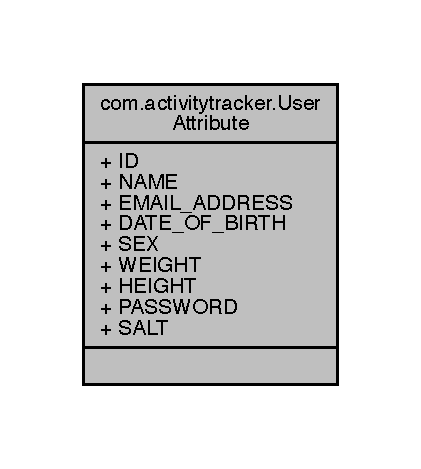
\includegraphics[width=202pt]{enumcom_1_1activitytracker_1_1_user_attribute__coll__graph}
\end{center}
\end{figure}
\subsection*{Public Attributes}
\begin{DoxyCompactItemize}
\item 
\mbox{\hyperlink{enumcom_1_1activitytracker_1_1_user_attribute_a82c5680d15b629e939afcd98a39abf76}{ID}}
\item 
\mbox{\hyperlink{enumcom_1_1activitytracker_1_1_user_attribute_aac51a5dfcaaa9e5304d37d74fc888af4}{N\+A\+ME}}
\item 
\mbox{\hyperlink{enumcom_1_1activitytracker_1_1_user_attribute_a8b9fa2ebf911262dfa24c683ff2a3b9c}{E\+M\+A\+I\+L\+\_\+\+A\+D\+D\+R\+E\+SS}}
\item 
\mbox{\hyperlink{enumcom_1_1activitytracker_1_1_user_attribute_af3b77ceae76c5f1c46e6821dc98940ee}{D\+A\+T\+E\+\_\+\+O\+F\+\_\+\+B\+I\+R\+TH}}
\item 
\mbox{\hyperlink{enumcom_1_1activitytracker_1_1_user_attribute_a53fe928fb805b69c606a351aac257558}{S\+EX}}
\item 
\mbox{\hyperlink{enumcom_1_1activitytracker_1_1_user_attribute_a024206b0dc3261031ef586b3f0fd530c}{W\+E\+I\+G\+HT}}
\item 
\mbox{\hyperlink{enumcom_1_1activitytracker_1_1_user_attribute_a0a80ca5cce8eb4494c2128bd4291a5b7}{H\+E\+I\+G\+HT}}
\item 
\mbox{\hyperlink{enumcom_1_1activitytracker_1_1_user_attribute_aa893eac0362a28e73a599ce1ba141d40}{P\+A\+S\+S\+W\+O\+RD}}
\item 
\mbox{\hyperlink{enumcom_1_1activitytracker_1_1_user_attribute_acd286be9d131a84a2be02e1cdac4c848}{S\+A\+LT}}
\end{DoxyCompactItemize}


\subsection{Detailed Description}
This enumeration type is used to specify the behaviour of generalized methods, particularly in the \mbox{\hyperlink{classcom_1_1activitytracker_1_1_d_b_manager}{D\+B\+Manager}} class. 

Definition at line 6 of file User\+Attribute.\+java.



\subsection{Member Data Documentation}
\mbox{\Hypertarget{enumcom_1_1activitytracker_1_1_user_attribute_af3b77ceae76c5f1c46e6821dc98940ee}\label{enumcom_1_1activitytracker_1_1_user_attribute_af3b77ceae76c5f1c46e6821dc98940ee}} 
\index{com\+::activitytracker\+::\+User\+Attribute@{com\+::activitytracker\+::\+User\+Attribute}!D\+A\+T\+E\+\_\+\+O\+F\+\_\+\+B\+I\+R\+TH@{D\+A\+T\+E\+\_\+\+O\+F\+\_\+\+B\+I\+R\+TH}}
\index{D\+A\+T\+E\+\_\+\+O\+F\+\_\+\+B\+I\+R\+TH@{D\+A\+T\+E\+\_\+\+O\+F\+\_\+\+B\+I\+R\+TH}!com\+::activitytracker\+::\+User\+Attribute@{com\+::activitytracker\+::\+User\+Attribute}}
\subsubsection{\texorpdfstring{D\+A\+T\+E\+\_\+\+O\+F\+\_\+\+B\+I\+R\+TH}{DATE\_OF\_BIRTH}}
{\footnotesize\ttfamily com.\+activitytracker.\+User\+Attribute.\+D\+A\+T\+E\+\_\+\+O\+F\+\_\+\+B\+I\+R\+TH}

Currently not used as no generalized method retrieves the user\textquotesingle{}s D\+OB. 

Definition at line 26 of file User\+Attribute.\+java.

\mbox{\Hypertarget{enumcom_1_1activitytracker_1_1_user_attribute_a8b9fa2ebf911262dfa24c683ff2a3b9c}\label{enumcom_1_1activitytracker_1_1_user_attribute_a8b9fa2ebf911262dfa24c683ff2a3b9c}} 
\index{com\+::activitytracker\+::\+User\+Attribute@{com\+::activitytracker\+::\+User\+Attribute}!E\+M\+A\+I\+L\+\_\+\+A\+D\+D\+R\+E\+SS@{E\+M\+A\+I\+L\+\_\+\+A\+D\+D\+R\+E\+SS}}
\index{E\+M\+A\+I\+L\+\_\+\+A\+D\+D\+R\+E\+SS@{E\+M\+A\+I\+L\+\_\+\+A\+D\+D\+R\+E\+SS}!com\+::activitytracker\+::\+User\+Attribute@{com\+::activitytracker\+::\+User\+Attribute}}
\subsubsection{\texorpdfstring{E\+M\+A\+I\+L\+\_\+\+A\+D\+D\+R\+E\+SS}{EMAIL\_ADDRESS}}
{\footnotesize\ttfamily com.\+activitytracker.\+User\+Attribute.\+E\+M\+A\+I\+L\+\_\+\+A\+D\+D\+R\+E\+SS}

The user\textquotesingle{}s email address.

Used in \mbox{\hyperlink{classcom_1_1activitytracker_1_1_d_b_manager_a20f726c054d6c8a6fc3ce629d87f1114}{D\+B\+Manager\+::get\+User\+String\+Attribute}} to specify that the user\textquotesingle{}s email address should be returned. 

Definition at line 22 of file User\+Attribute.\+java.

\mbox{\Hypertarget{enumcom_1_1activitytracker_1_1_user_attribute_a0a80ca5cce8eb4494c2128bd4291a5b7}\label{enumcom_1_1activitytracker_1_1_user_attribute_a0a80ca5cce8eb4494c2128bd4291a5b7}} 
\index{com\+::activitytracker\+::\+User\+Attribute@{com\+::activitytracker\+::\+User\+Attribute}!H\+E\+I\+G\+HT@{H\+E\+I\+G\+HT}}
\index{H\+E\+I\+G\+HT@{H\+E\+I\+G\+HT}!com\+::activitytracker\+::\+User\+Attribute@{com\+::activitytracker\+::\+User\+Attribute}}
\subsubsection{\texorpdfstring{H\+E\+I\+G\+HT}{HEIGHT}}
{\footnotesize\ttfamily com.\+activitytracker.\+User\+Attribute.\+H\+E\+I\+G\+HT}

The user\textquotesingle{}s height (in metres).

Used in \mbox{\hyperlink{classcom_1_1activitytracker_1_1_d_b_manager_a98df66254bec4d74b29cfe468a9fc794}{D\+B\+Manager\+::get\+User\+Float\+Attribute}} to specify that the user\textquotesingle{}s email height should be returned. 

Definition at line 42 of file User\+Attribute.\+java.

\mbox{\Hypertarget{enumcom_1_1activitytracker_1_1_user_attribute_a82c5680d15b629e939afcd98a39abf76}\label{enumcom_1_1activitytracker_1_1_user_attribute_a82c5680d15b629e939afcd98a39abf76}} 
\index{com\+::activitytracker\+::\+User\+Attribute@{com\+::activitytracker\+::\+User\+Attribute}!ID@{ID}}
\index{ID@{ID}!com\+::activitytracker\+::\+User\+Attribute@{com\+::activitytracker\+::\+User\+Attribute}}
\subsubsection{\texorpdfstring{ID}{ID}}
{\footnotesize\ttfamily com.\+activitytracker.\+User\+Attribute.\+ID}

Currently not used as no generalized method retrieves the user\textquotesingle{}s ID. 

Definition at line 10 of file User\+Attribute.\+java.

\mbox{\Hypertarget{enumcom_1_1activitytracker_1_1_user_attribute_aac51a5dfcaaa9e5304d37d74fc888af4}\label{enumcom_1_1activitytracker_1_1_user_attribute_aac51a5dfcaaa9e5304d37d74fc888af4}} 
\index{com\+::activitytracker\+::\+User\+Attribute@{com\+::activitytracker\+::\+User\+Attribute}!N\+A\+ME@{N\+A\+ME}}
\index{N\+A\+ME@{N\+A\+ME}!com\+::activitytracker\+::\+User\+Attribute@{com\+::activitytracker\+::\+User\+Attribute}}
\subsubsection{\texorpdfstring{N\+A\+ME}{NAME}}
{\footnotesize\ttfamily com.\+activitytracker.\+User\+Attribute.\+N\+A\+ME}

The user\textquotesingle{}s full name.

Used in \mbox{\hyperlink{classcom_1_1activitytracker_1_1_d_b_manager_a20f726c054d6c8a6fc3ce629d87f1114}{D\+B\+Manager\+::get\+User\+String\+Attribute}} to specify that the user\textquotesingle{}s name should be returned. 

Definition at line 16 of file User\+Attribute.\+java.

\mbox{\Hypertarget{enumcom_1_1activitytracker_1_1_user_attribute_aa893eac0362a28e73a599ce1ba141d40}\label{enumcom_1_1activitytracker_1_1_user_attribute_aa893eac0362a28e73a599ce1ba141d40}} 
\index{com\+::activitytracker\+::\+User\+Attribute@{com\+::activitytracker\+::\+User\+Attribute}!P\+A\+S\+S\+W\+O\+RD@{P\+A\+S\+S\+W\+O\+RD}}
\index{P\+A\+S\+S\+W\+O\+RD@{P\+A\+S\+S\+W\+O\+RD}!com\+::activitytracker\+::\+User\+Attribute@{com\+::activitytracker\+::\+User\+Attribute}}
\subsubsection{\texorpdfstring{P\+A\+S\+S\+W\+O\+RD}{PASSWORD}}
{\footnotesize\ttfamily com.\+activitytracker.\+User\+Attribute.\+P\+A\+S\+S\+W\+O\+RD}

The user\textquotesingle{}s encrypted password hash.

Used in \mbox{\hyperlink{classcom_1_1activitytracker_1_1_d_b_manager_a20f726c054d6c8a6fc3ce629d87f1114}{D\+B\+Manager\+::get\+User\+String\+Attribute}} to specify that the user\textquotesingle{}s password hash should be returned. 

Definition at line 48 of file User\+Attribute.\+java.

\mbox{\Hypertarget{enumcom_1_1activitytracker_1_1_user_attribute_acd286be9d131a84a2be02e1cdac4c848}\label{enumcom_1_1activitytracker_1_1_user_attribute_acd286be9d131a84a2be02e1cdac4c848}} 
\index{com\+::activitytracker\+::\+User\+Attribute@{com\+::activitytracker\+::\+User\+Attribute}!S\+A\+LT@{S\+A\+LT}}
\index{S\+A\+LT@{S\+A\+LT}!com\+::activitytracker\+::\+User\+Attribute@{com\+::activitytracker\+::\+User\+Attribute}}
\subsubsection{\texorpdfstring{S\+A\+LT}{SALT}}
{\footnotesize\ttfamily com.\+activitytracker.\+User\+Attribute.\+S\+A\+LT}

Currently not used as no generalized method retrieves the user\textquotesingle{}s password encryption salt. 

Definition at line 52 of file User\+Attribute.\+java.

\mbox{\Hypertarget{enumcom_1_1activitytracker_1_1_user_attribute_a53fe928fb805b69c606a351aac257558}\label{enumcom_1_1activitytracker_1_1_user_attribute_a53fe928fb805b69c606a351aac257558}} 
\index{com\+::activitytracker\+::\+User\+Attribute@{com\+::activitytracker\+::\+User\+Attribute}!S\+EX@{S\+EX}}
\index{S\+EX@{S\+EX}!com\+::activitytracker\+::\+User\+Attribute@{com\+::activitytracker\+::\+User\+Attribute}}
\subsubsection{\texorpdfstring{S\+EX}{SEX}}
{\footnotesize\ttfamily com.\+activitytracker.\+User\+Attribute.\+S\+EX}

Currently not used as no generalized method retrieves the user\textquotesingle{}s sex. 

Definition at line 30 of file User\+Attribute.\+java.

\mbox{\Hypertarget{enumcom_1_1activitytracker_1_1_user_attribute_a024206b0dc3261031ef586b3f0fd530c}\label{enumcom_1_1activitytracker_1_1_user_attribute_a024206b0dc3261031ef586b3f0fd530c}} 
\index{com\+::activitytracker\+::\+User\+Attribute@{com\+::activitytracker\+::\+User\+Attribute}!W\+E\+I\+G\+HT@{W\+E\+I\+G\+HT}}
\index{W\+E\+I\+G\+HT@{W\+E\+I\+G\+HT}!com\+::activitytracker\+::\+User\+Attribute@{com\+::activitytracker\+::\+User\+Attribute}}
\subsubsection{\texorpdfstring{W\+E\+I\+G\+HT}{WEIGHT}}
{\footnotesize\ttfamily com.\+activitytracker.\+User\+Attribute.\+W\+E\+I\+G\+HT}

The user\textquotesingle{}s weight (in kilograms).

Used in \mbox{\hyperlink{classcom_1_1activitytracker_1_1_d_b_manager_a98df66254bec4d74b29cfe468a9fc794}{D\+B\+Manager\+::get\+User\+Float\+Attribute}} to specify that the user\textquotesingle{}s email weight should be returned. 

Definition at line 36 of file User\+Attribute.\+java.



The documentation for this enum was generated from the following file\+:\begin{DoxyCompactItemize}
\item 
app/src/com/activitytracker/\mbox{\hyperlink{_user_attribute_8java}{User\+Attribute.\+java}}\end{DoxyCompactItemize}

\chapter{File Documentation}
\hypertarget{_activity_tracker_8java}{}\section{app/src/com/activitytracker/\+Activity\+Tracker.java File Reference}
\label{_activity_tracker_8java}\index{app/src/com/activitytracker/\+Activity\+Tracker.\+java@{app/src/com/activitytracker/\+Activity\+Tracker.\+java}}
\subsection*{Classes}
\begin{DoxyCompactItemize}
\item 
class \hyperlink{classcom_1_1activitytracker_1_1_activity_tracker}{com.\+activitytracker.\+Activity\+Tracker}
\end{DoxyCompactItemize}
\subsection*{Packages}
\begin{DoxyCompactItemize}
\item 
package \hyperlink{namespacecom_1_1activitytracker}{com.\+activitytracker}
\end{DoxyCompactItemize}

\hypertarget{_create_user_window_8java}{}\section{app/src/com/activitytracker/\+Create\+User\+Window.java File Reference}
\label{_create_user_window_8java}\index{app/src/com/activitytracker/\+Create\+User\+Window.\+java@{app/src/com/activitytracker/\+Create\+User\+Window.\+java}}
\subsection*{Classes}
\begin{DoxyCompactItemize}
\item 
class \hyperlink{classcom_1_1activitytracker_1_1_create_user_window}{com.\+activitytracker.\+Create\+User\+Window}
\end{DoxyCompactItemize}
\subsection*{Packages}
\begin{DoxyCompactItemize}
\item 
package \hyperlink{namespacecom_1_1activitytracker}{com.\+activitytracker}
\end{DoxyCompactItemize}

\hypertarget{_d_b_manager_8java}{}\section{app/src/com/activitytracker/\+D\+B\+Manager.java File Reference}
\label{_d_b_manager_8java}\index{app/src/com/activitytracker/\+D\+B\+Manager.\+java@{app/src/com/activitytracker/\+D\+B\+Manager.\+java}}
\subsection*{Classes}
\begin{DoxyCompactItemize}
\item 
class \hyperlink{classcom_1_1activitytracker_1_1_d_b_manager}{com.\+activitytracker.\+D\+B\+Manager}
\end{DoxyCompactItemize}
\subsection*{Packages}
\begin{DoxyCompactItemize}
\item 
package \hyperlink{namespacecom_1_1activitytracker}{com.\+activitytracker}
\end{DoxyCompactItemize}

\hypertarget{_iteration3_test_8java}{}\section{app/src/com/activitytracker/\+Iteration3\+Test.java File Reference}
\label{_iteration3_test_8java}\index{app/src/com/activitytracker/\+Iteration3\+Test.\+java@{app/src/com/activitytracker/\+Iteration3\+Test.\+java}}
\subsection*{Classes}
\begin{DoxyCompactItemize}
\item 
class \hyperlink{classcom_1_1activitytracker_1_1_iteration3_test}{com.\+activitytracker.\+Iteration3\+Test}
\end{DoxyCompactItemize}
\subsection*{Packages}
\begin{DoxyCompactItemize}
\item 
package \hyperlink{namespacecom_1_1activitytracker}{com.\+activitytracker}
\end{DoxyCompactItemize}

\hypertarget{_login_window_8java}{}\section{app/src/com/activitytracker/\+Login\+Window.java File Reference}
\label{_login_window_8java}\index{app/src/com/activitytracker/\+Login\+Window.\+java@{app/src/com/activitytracker/\+Login\+Window.\+java}}
\subsection*{Classes}
\begin{DoxyCompactItemize}
\item 
class \hyperlink{classcom_1_1activitytracker_1_1_login_window}{com.\+activitytracker.\+Login\+Window}
\end{DoxyCompactItemize}
\subsection*{Packages}
\begin{DoxyCompactItemize}
\item 
package \hyperlink{namespacecom_1_1activitytracker}{com.\+activitytracker}
\end{DoxyCompactItemize}

\hypertarget{_main_window_8java}{}\section{app/src/com/activitytracker/\+Main\+Window.java File Reference}
\label{_main_window_8java}\index{app/src/com/activitytracker/\+Main\+Window.\+java@{app/src/com/activitytracker/\+Main\+Window.\+java}}
\subsection*{Classes}
\begin{DoxyCompactItemize}
\item 
class \mbox{\hyperlink{classcom_1_1activitytracker_1_1_main_window}{com.\+activitytracker.\+Main\+Window}}
\end{DoxyCompactItemize}
\subsection*{Packages}
\begin{DoxyCompactItemize}
\item 
package \mbox{\hyperlink{namespacecom_1_1activitytracker}{com.\+activitytracker}}
\end{DoxyCompactItemize}

\hypertarget{_run_8java}{}\section{app/src/com/activitytracker/\+Run.java File Reference}
\label{_run_8java}\index{app/src/com/activitytracker/\+Run.\+java@{app/src/com/activitytracker/\+Run.\+java}}
\subsection*{Classes}
\begin{DoxyCompactItemize}
\item 
class \hyperlink{classcom_1_1activitytracker_1_1_run}{com.\+activitytracker.\+Run}
\end{DoxyCompactItemize}
\subsection*{Packages}
\begin{DoxyCompactItemize}
\item 
package \hyperlink{namespacecom_1_1activitytracker}{com.\+activitytracker}
\end{DoxyCompactItemize}

\hypertarget{_run_attribute_8java}{}\section{app/src/com/activitytracker/\+Run\+Attribute.java File Reference}
\label{_run_attribute_8java}\index{app/src/com/activitytracker/\+Run\+Attribute.\+java@{app/src/com/activitytracker/\+Run\+Attribute.\+java}}
\subsection*{Classes}
\begin{DoxyCompactItemize}
\item 
enum \mbox{\hyperlink{enumcom_1_1activitytracker_1_1_run_attribute}{com.\+activitytracker.\+Run\+Attribute}}
\end{DoxyCompactItemize}
\subsection*{Packages}
\begin{DoxyCompactItemize}
\item 
package \mbox{\hyperlink{namespacecom_1_1activitytracker}{com.\+activitytracker}}
\end{DoxyCompactItemize}

\hypertarget{_secure_string_8java}{}\section{app/src/com/activitytracker/\+Secure\+String.java File Reference}
\label{_secure_string_8java}\index{app/src/com/activitytracker/\+Secure\+String.\+java@{app/src/com/activitytracker/\+Secure\+String.\+java}}
\subsection*{Classes}
\begin{DoxyCompactItemize}
\item 
class \hyperlink{classcom_1_1activitytracker_1_1_secure_string}{com.\+activitytracker.\+Secure\+String}
\end{DoxyCompactItemize}
\subsection*{Packages}
\begin{DoxyCompactItemize}
\item 
package \hyperlink{namespacecom_1_1activitytracker}{com.\+activitytracker}
\end{DoxyCompactItemize}

\hypertarget{_user_8java}{}\section{app/src/com/activitytracker/\+User.java File Reference}
\label{_user_8java}\index{app/src/com/activitytracker/\+User.\+java@{app/src/com/activitytracker/\+User.\+java}}
\subsection*{Classes}
\begin{DoxyCompactItemize}
\item 
class \hyperlink{classcom_1_1activitytracker_1_1_user}{com.\+activitytracker.\+User}
\item 
enum \hyperlink{enumcom_1_1activitytracker_1_1_user_1_1_sex}{com.\+activitytracker.\+User.\+Sex}
\end{DoxyCompactItemize}
\subsection*{Packages}
\begin{DoxyCompactItemize}
\item 
package \hyperlink{namespacecom_1_1activitytracker}{com.\+activitytracker}
\end{DoxyCompactItemize}

\hypertarget{_user_attribute_8java}{}\section{app/src/com/activitytracker/\+User\+Attribute.java File Reference}
\label{_user_attribute_8java}\index{app/src/com/activitytracker/\+User\+Attribute.\+java@{app/src/com/activitytracker/\+User\+Attribute.\+java}}
\subsection*{Classes}
\begin{DoxyCompactItemize}
\item 
enum \hyperlink{enumcom_1_1activitytracker_1_1_user_attribute}{com.\+activitytracker.\+User\+Attribute}
\end{DoxyCompactItemize}
\subsection*{Packages}
\begin{DoxyCompactItemize}
\item 
package \hyperlink{namespacecom_1_1activitytracker}{com.\+activitytracker}
\end{DoxyCompactItemize}

%--- End generated contents ---

% Index
\backmatter
\newpage
\phantomsection
\clearemptydoublepage
\addcontentsline{toc}{chapter}{Index}
\printindex

\end{document}
